%%%%%%%%%%%%%%%%%%%%%%%%%%%%%%%%%%%%%%%%%%%%
%%%%%%%%%%%%%%%%%%%%%%%%%%%%%%%%%%%%%%%%%%%%
% Import preamble
\documentclass[aspectratio=169,xcolor=dvipsnames, 11pt]{beamer} 

%\documentclass[xcolor=dvipsnames,mathserif]{beamer} % this option has curvier math
%\documentclass[xcolor=dvipsnames,11pt]{beamer}
% Note: the color structure needs to be added here in the title. Now it recognizes all beamer % colors.

%%%%%%%%  PRESENTATION LAYOUT:
\usepackage{appendixnumberbeamer} % this package does not count the appendix pages.
\mode<presentation>
{
  \usetheme{Boadilla}
  \usecolortheme{lily} % lily is nice or orchid but not for definition
  \setbeamercovered{invisible}
  \setbeamertemplate{footline}{\raggedleft\insertframenumber~/~\inserttotalframenumber\hspace*{3pt}\vskip3pt} %this command shows frame number, not page number at bottom (means if using overlays, % frame number does not change)
%\setbeamertemplate{footline}[page number]  % this puts only page number on bottom
 \setbeamertemplate{navigation symbols}{}  % this erases navigation symbols.
 \setbeamersize{text margin left=0.2cm, text margin right=0.1cm}
 \setbeamertemplate{frametitle}[default][center]
 \setbeamercolor{frametitle}{fg=black}
 \setbeamerfont{frametitle}{size=\large, series=\bfseries} % Modifies frame title font.
 \setbeamercolor{button}{fg=blue, bg=white}
 \setbeamertemplate{itemize item}[circle]
 \setbeamercolor{itemize item}{fg=black}
 \setbeamercolor{itemize/enumerate body}{fg=black}
 \setbeamerfont{framesubtitle}{series=\mdseries}

}

\renewcommand{\familydefault}{\rmdefault} %Options here are \ttdefault \ssdefault or \rmdefault.

% This defines actual color palette; 
\definecolor{blue}{RGB}{0,114,178}
\definecolor{red}{RGB}{213,94,0}
\definecolor{yellow}{RGB}{240,228,66}
\definecolor{green}{RGB}{0,158,115}
\definecolor{orange}{RGB}{230,159,0}

\hypersetup{
  colorlinks = false,
  linkbordercolor = {white},
  linkcolor = {blue}
}

%%% Color customization: where these colors are used. 
\colorlet{cwords}{blue} %this defines a color, stored under the name cwords that will be used and recognized in document.
\colorlet{cwordsc}{red} %color for contrast with some other word.
\colorlet{cwords2}{green} %2nd color for contrast with some other word.
\colorlet{cmath}{blue} %color for math in text.
%\everymath{\color{blue}} % This in conjunction with the everysel package sets color of math
\everydisplay{\color{blue}}


%%%%%%%%  PACKAGES USED:
\usepackage{amsmath}
\usepackage{setspace} % Only needed for spacing
\usepackage{changepage} % Only needed for local margin setting
\usepackage{mathpazo}% font, is overwritten by times
%\usepackage[hypertexnames=false]{hyperref} %This makes hyperref ``dumber'', and, hence, more robust! (otherwise sometimes the appendix links don't work).
\usepackage{hyperref}
\usepackage{multimedia}
\usepackage[english]{babel}
\usepackage{graphicx}
\usepackage{caption}
%\usepackage{subfig}
\usepackage{subfloat}
\usepackage[en-US]{datetime2}
\usepackage{tabulary}
\usepackage{tabularx}
\usepackage{array,booktabs} % Needed for esttab tables according to the "inequality survey."
\newcommand{\sym}[1]{{#1}} % for symbols in Table
\usepackage[T1]{fontenc}
\usepackage[utf8]{inputenc}
\usepackage{times} % This is a different font.
\usepackage[overlay,absolute]{textpos}
%%%\usepackage{animate} % Animate graphs BUG
\setlength{\TPHorizModule}{1cm}
\setlength{\TPVertModule}{1cm}
\captionsetup[figure]{labelformat=empty} % removes caption prefix figure
\setlength{\itemsep}{\fill} % this is supposed to stretch items across full frame.
%\setlength{\parskip}{0.8\baselineskip} % This affects spacing between normal lines (not itemized).
\usepackage{colortbl} % For cell colors
\usepackage[final]{pdfpages}
\usepackage{caption}
\usepackage{subcaption}
%\captionsetup{justification   = raggedright,
%              singlelinecheck = false}
%\usepackage{adjustbox} % to use resizebox for tables size.
\usepackage[export]{adjustbox} % to use resizebox for tables size.
\usepackage{eurosym}
\usepackage{gensymb}

%% TIKZ
\usepackage{tikz}
\usetikzlibrary{er, positioning,decorations.pathmorphing,calc}
\usepackage{tikzscale}

\tikzset{every entity/.style={draw=black, fill=white}}
\tikzset{comment/.style={draw=white, fill=white}}
\tikzset{
	invisible/.style={opacity=0},
	visible on/.style={alt=#1{}{invisible}},
	alt/.code args={<#1>#2#3}{%
		\alt<#1>{\pgfkeysalso{#2}}{\pgfkeysalso{#3}} % \pgfkeysalso doesn't change the path
	},
}

% Commands from template
\newcommand{\alrt}[1]{{\color{alert} #1}}
\newcommand{\alrtl}[1]{{\color{alert}\large #1}}
\newcommand{\alrtL}[1]{{\color{alert}\Large #1}}
\newcommand{\struc}[1]{{\color{structure} #1}}
\newcommand{\strucL}[1]{{\color{structure}\Large #1}}
\newcommand{\strucl}[1]{{\color{structure}\large #1}}
\newcommand{\dred}[1]{{\color{darkred} #1}}
\newcommand{\dredl}[1]{{\color{darkred}\large #1}}
\newcommand{\dredL}[1]{{\color{darkred}\Large #1}}
\newcommand{\altc}[1]{{\color{darkgreen}\textbf{#1}}}
\newcommand{\altcl}[1]{{\color{darkgreen}\textbf{\large #1}}}
\newcommand{\altcL}[1]{{\color{darkgreen}\textbf{\Large #1}}}
\newcommand{\hush}{\hushit}
\newcommand{\hushalrt}[1]{\hushit{{\color{alert} #1}}}
\newcommand{\hushalrtl}[1]{\hushit{{\large\color{alert} #1}}}
\newcommand{\hushalrtL}[1]{\hushit{{\Large\color{alert} #1}}}
\newcommand{\hushstruc}[1]{\hushit{{\color{structure} #1}}}
\newcommand{\hushstrucl}[1]{\hushit{{\large\color{structure} #1}}}
\newcommand{\hushstrucL}[1]{\hushit{{\Large\color{structure} #1}}}


\setbeamertemplate{caption}[numbered]

%%%%%%%%%SECTION TITLES DISPLAYED ON FULL PAGE %%%%%%%%%%
%%%%%%%%%%%%%%%%%%%%%%%%%%%%%%%%%%%%%%%%%%%
\AtBeginSection[]{
  \begin{frame}
  \vfill
  \centering
  \begin{beamercolorbox}[sep=8pt,center,shadow=true,rounded=true]{title}
    \usebeamerfont{title}{\huge \color{red} \insertsectionhead} \par
  \end{beamercolorbox}
  \vfill
  \end{frame}
}

\AtBeginSubsection[]{
  \begin{frame}
  \vfill
  \centering
  \begin{beamercolorbox}[sep=8pt,center,shadow=true,rounded=true]{title}
    \usebeamerfont{title}{\huge \color{blue} \insertsubsectionhead} \par
  \end{beamercolorbox}
  \vfill
  \end{frame}
}

%
% Custom font for a frame.
%
\usepackage{environ}
\newcommand{\customframefont}[1]{
\setbeamertemplate{itemize/enumerate body begin}{#1}
\setbeamertemplate{itemize/enumerate subbody begin}{#1}
}

\NewEnviron{framefont}[1]{
\customframefont{#1} % for itemize/enumerate
{#1 % For the text outside itemize/enumerate
\BODY
}
\customframefont{\normalsize}
}

%%%%%%%%%%%%%%%%%%%%%%%%%%%%%%%%%%%%%%%%%%%%%%%%%%%%%%%
%%%%%% OTHER PIECES OF TEMPLATE FILE
%%%%%% DELETE ONCE CLEAR THAT NOTHING IS MISSING
%%%%%%%%%%%%%%%%%%%%%%%%%%%%%%%%%%%%%%%%%%%%%%%%%%%%%%%


%\documentclass[aspectratio=169]{beamer} % wide
%\usepackage{amsmath,amsthm,fancyhdr,setspace,graphicx,booktabs,pdflscape}
%\usepackage{geometry}
%\usepackage{etex}
%\usepackage{xcolor,colortbl}
%\usepackage{beamerprosper}
%\usepackage{url}
%\usepackage{enumerate}
%\usepackage{graphicx}
%\usepackage{hyperref}
%\usepackage{multicol}
%\usepackage{caption}
%\usepackage{beamerprosper}
%\usepackage{pgfpages, pdfpages}
%\usepackage{tikz-cd}
%
%\usepackage{tabularx}
%\usepackage{anyfontsize}
%\usepackage{multicol,tabto}
%
%\usepackage{float}
%\usepackage{soul}
%\usepackage{grffile}
%\usepackage{changepage}
%\usepackage{sansmathaccent}
%\pdfmapfile{+sansmathaccent.map}
%
%
%\usetikzlibrary{er,positioning,calc,decorations.pathreplacing}
%
%\mode<presentation>
%\usefonttheme{structuresmallcapsserif}
%\setbeamertemplate{footline}[frame number]{}
%\setbeamertemplate{navigation symbols}{}
%
%%change font
%\usefonttheme{default}
%\setbeamertemplate{footline}[frame number]{}
%\setbeamertemplate{navigation symbols}{}
%
%\newcommand{\fig}[3]{\begin{frame}\frametitle{#2}\centerline{\includegraphics[width=#3in]{#1}}\end{frame}}
%
%\newcommand{\blackslide}[1]{\beamersetaveragebackground{black}\begin{frame}\frametitle{}\end{frame}\beamersetaveragebackground{white}}
%
%% pause commands
%\newcommand{\m}[2]{\begin{frame}\frametitle{#1}{ #2}\end{frame}}
%\newcommand{\mm}[3]{\begin{frame}\frametitle{#1}\uncover<1->{ #2}\uncover<2->{ #3 }\end{frame}}
%\newcommand{\mmm}[4]{\begin{frame}\frametitle{#1}\uncover<1->{ #2}\uncover<2->{ #3 }\uncover<3->{ #4 }\end{frame}}
%\newcommand{\mmmm}[5]{\begin{frame}\frametitle{#1}\uncover<1->{ #2}\uncover<2->{ #3 }\uncover<3->{ #4 }\uncover<4->{ #5 }\end{frame}}
%
%\setlength{\footskip}{24pt}
%
%\newcommand{\ex}{\mathbf{E}}
%\newcommand{\cov}{\mathbb{C}}
%\newcommand{\var}{\mathbb{V}}
%\newcommand{\tu}{\overline{\theta}}
%\newcommand{\vu}{\overline{v}}
%\newcommand{\tl}{\underline{\theta}}
%\newcommand{\ab}{\bar{a}}
%\newcommand{\lb}{\bar{L}}
%\newcommand{\hb}{\bar{H}}
%
%% New colors.
%\definecolor{darkred}{rgb}{0.6,0,0}
%\definecolor{darkblue}{rgb}{.15,.25,.55}
%\definecolor{darkgreen}{rgb}{0,.35,.05}
%\definecolor{ltgreen}{rgb}{0,.05,.8}
%\definecolor{bred}{rgb}{1,0,.05}
%\definecolor{navy}{rgb}{.1,.1,.5}
%
%% from beamer lecture 
%
%\newtheorem{proposition}{Proposition}
%%\newtheorem{theorem}{Theorem}
%
%\newenvironment{changemargin}[2]{%
%    \begin{list}{}{ %
%%        \setlength{\topmargin}{#3}%
%            \setlength{\topsep}{0pt}%
%            \setlength{\leftmargin}{#1}%
%            \setlength{\rightmargin}{#2}%
%            \setlength{\listparindent}{\parindent}%
%            \setlength{\itemindent}{\parindent}%
%            \setlength{\parsep}{\parskip}%
%        }%
%\item[]}{\end{list}}
%
%%Allows us to force a column width in array environment
%\newcolumntype{C}[1]{>{\centering\arraybackslash}p{#1}}
%\newcolumntype{L}[1]{>{\raggedright\arraybackslash}p{#1}}
%\newcolumntype{R}[1]{>{\raggedleft\arraybackslash}p{#1}}

%%SHORTCUTS

%%%%%%%%%%%%%%%%%%%%%%%%%
%% Bullets
%%%%%%%%%%%%%%%%%%%%%%%%%

\newcommand{\p}{\item}
\newcommand{\ip}{\item[]} % Invisible items.
\newcommand{\bb}{\begin{itemize}\itemsep15pt}
\newcommand{\bbs}{\medskip \begin{itemize}\itemsep10pt}
\newcommand{\bbvs}{\medskip \begin{itemize}\itemsep3pt}
\newcommand{\ee}{\end{itemize}}

\newcommand{\ben}{\begin{enumerate}}
\newcommand{\een}{\end{enumerate}}


\newcommand{\can}{\citeasnoun}
\newcommand{\ican}{\iciteasnoun}

\newcommand{\non}{\nonumber}

%%%%%%%%%%%%%%%%%%%%%%%%%
%% Derivatives and partials. 
%%%%%%%%%%%%%%%%%%%%%%%%%
%% Duplicate: two ways to get partials
\newcommand{\pa}[2]{\frac{\partial #1}{\partial #2}} % Stef
\newcommand{\pder}[2]{\frac{\partial #1}{\partial #2}} % Doug

\newcommand{\dneu}{\mbox{d}}
\newcommand{\di}[2]{\frac{\dneu #1}{\dneu #2}}
%% Duplicate: two ways to get derivatives.
\newcommand{\dd}[2]{\frac{d #1}{d #2}} % Stef version
\newcommand{\der}[2]{\frac{d#1}{d#2}} % Doug version

%%%%%%%%%%%%%%%%%%%%%%%%%
%% Brackets and fractions
%%%%%%%%%%%%%%%%%%%%%%%%%


\newcommand{\fr}[2]{\frac{#1}{#2}}
\newcommand{\pfr}[2]{\left(\frac{#1}{#2}\right)}
\newcommand{\bfr}[2]{\left[\frac{#1}{#2}\right]}
\newcommand{\cfr}[2]{\left\{\frac{#1}{#2}\right\}}

\newcommand{\pr}[1]{\left(#1\right)}
\newcommand{\br}[1]{\left[#1\right]}
\newcommand{\cb}[1]{\left\{#1\right\}}
\newcommand{\qand}{\quad\text{and}\quad}


%%%%%%%%%%%%%%%%%%%%%%%%%
%% ARROWS
%%%%%%%%%%%%%%%%%%%%%%%%%

\newcommand{\Ra}{\Rightarrow}
\newcommand{\ra}{\rightarrow}
\newcommand{\Ras}{\ \Rightarrow\ }
\newcommand{\ras}{\ \rightarrow\ }
\newcommand{\Raq}{\quad\Rightarrow\quad}
\newcommand{\raq}{\quad\rightarrow\quad}


%%%%%%%%%%%%%%%%%%%%%%%%%
%% MATH
%%%%%%%%%%%%%%%%%%%%%%%%%

\newcommand{\E}[1]{\mathbb{E}\br{#1}}
\newcommand{\eps}{\varepsilon}

\newcommand{\be}{\begin{equation}}
\newcommand{\eeq}{\end{equation}}

\newcommand{\bea}{\begin{eqnarray}}
\newcommand{\eea}{\end{eqnarray}}

\newcommand{\bean}{\begin{eqnarray*}}
\newcommand{\eean}{\end{eqnarray*}}

\newcommand{\ba}{\begin{array}}
\newcommand{\ea}{\end{array}}


\newcommand{\lb}{\linebreak}
\newcommand{\strich}[2]{\left. #1 \right|_{#2}}
% use \left. before


%\newcommand{\bean}{\begin{multline*}}
%\newcommand{\eean}{\end{multline*}}

\newcommand{\nl}{\newline}
\newcommand{\np}{\newpage}

\newcommand{\rf}[1]{(\ref{#1})}



\newcommand{\ds}{\displaystyle}
\newcommand{\fn}{\footnote}

\newcommand{\var}{\mbox{Var}}
\newcommand{\cov}{\mbox{Cov}}

\newcommand{\il}{\int\limits}

\newcommand{\li}{\left}
\newcommand{\re}{\right}

\newcommand{\s}{\right|_}

\newcommand{\ambigo}{\ba{c}>\\[-3mm]<\ea}
\newcommand{\ambigu}{\ba{c}<\\[-3mm]>\ea}

\newcommand{\ul}{\underline}
\newcommand{\ol}{\overline}

\newcommand{\e}{\mbox{\euro{} }}

%%%%%%%%%%%%%%%%%%%%%%%%%%%%%%%%%%%%%%%%%%%%
%%%%%%%%%%%%%%%%%%%%%%%%%%%%%%%%%%%%%%%%%%%%
% Define title


%\title{Climate survey - France}
%\author[OECD]{ \\  Antoine Dechezleprêtre, Adrien Fabre, Bluebery Planterose, Stefanie Stantcheva \\ (OECD) }
%
%              \date{}
              
\begin{document}



%%%%%%%%%%%%%%%%%%%%%%%%%%%%%%%%%%%%%%%%%%%%
%%%%%%%%%%%%%%%%%%%%%%%%%%%%%%%%%%%%%%%%%%%%
% Begin of the document
% TITLE PAGE

\begin{frame}
\thispagestyle{empty}
\begin{center}
\begin{LARGE}
\textcolor{blue}{Climate survey - France}
\end{LARGE}

\vspace{1cm}


Laurence Boone, Antoine Dechezleprêtre, Adrien Fabre, Tobias Kruse, Bluebery Planterose, Ana Sanchez-Chico, Stefanie Stantcheva \\

%\vspace{-0.3cm}
OECD/CAE \\

\DTMlangsetup{showdayofmonth=false}
\textit{\today} 

\end{center}

\bigskip

\end{frame}

% Section Survey and Data: 
% Need to describe i) sample ii) survey blocks —> refer to online Appendix for questionnaires in original language (we would need them all nicely formatted) + survey link if available (but not the one we are actually using to collect data, rather we need a mock one)

% Section Knowledge: 

% Split into: What are key things that people misperceive? 
% What are things that they are relatively well aware of?

% One section on “Who has better knowledge?” Just a regression of some summary measure of knowledge on individual characteristics. 

% Policy message of this section 
% Who knows more? Where is key info lacking (that policy makers should fix).  

% Section on who supports climate change policies. 

% Regress Outcomes on set A and set B. Identify main patterns. 
% In Appendix: Full regression tables. 
% In paper: 4-5 of they key heterogeneities, shown in graphical format. For instance, Tobias already identified that driving and relying on energy was important; Adrien pointed to age. 

% LDA analysis to identify “types” of respondents. Perhaps in Appendix by country, in main paper all countries pooled? 

% Section on what makes people support climate change policies

% A. Mechanisms. 
% Regress Outcomes on set C + set A (—> answers the question of what type of thinking needs to changed 
% (We already did nice figures like this, but we needed to reorganize what was a mechanism and what was an outcome) 

% B. Gelbach decompositions of the key heterogeneities (e.g.: what makes people of different ages support different policies) into the mechanisms of set C. 

% C. Provide description of Treatments with screen shots. 
% Regress Outcomes on treatment indicators + set A. 


\begin{frame}{Motivation}
\bbs
\ip Climate policies have been difficult to pass.
\ip The design of climate policies needs to account for the political economy and public acceptability.
\ip \textcolor{blue}{Resistance to climate policies} arises largely from:
\bbs
\ip Legitimate concerns about \textcolor{blue}{distributional and lifestyle impacts}
\ip \textcolor{blue}{Misconceptions} about the impacts of climate change and the effects of climate policies on the economy and the environment
\ee 
\ip Addressing concerns and misconceptions may be difficult, as they are influenced by personal attributes, country specificities and political views.
\ee
\end{frame}

\begin{frame}{Project objectives}
\bbs
\ip \textcolor{blue}{Overall goal:} contribute to construct country-specific advice on policies to deal with the transition to a low-carbon economy by understanding people’s perceptions about climate change and preferences over available climate policies.
\ip \textcolor{blue}{Research questions:}
\bbs
\ip How social attitudes, values, and perceptions drive support or opposition for climate policies across socio-economic groups?
\ip How social preferences on climate change mitigation policies differ between countries?
\ip How perceptions may change after receiving new information on the effects of policies/climate change (in a video format) and how it translates into beliefs and support?
\ee
\ee
\end{frame}

\begin{frame}{An international survey}
\bbvs
\ip \textcolor{blue}{Large-scale cross-country survey} to analyse attitudes on climate change and climate policies.
\ip Wide country coverage:
\bbvs
\ip \textcolor{blue}{20 countries} in all world regions, low-income as well as high-income, 
\ip \textcolor{blue}{covering 72\% of global CO$_\text{2}$ emissions}, including 18 out of the 21 largest polluters.
\ee
\ee
\makebox[\textwidth][c]{ \includegraphics[width=.6\textwidth]{"../figures/Country_coverage"}}
\end{frame}

\begin{frame}{Method: Large-scale Social Economics Surveys and Experiments}
\bb
\ip \textcolor{magenta}{Surveys are a key tool:}
\bbs 
\ip Some aspects cannot be perceived in other data, not matter how good they are: Perceptions, attitudes, knowledge, views.
\ip Revealed preference with observational data has limits (data and assumptions required).

\ip Unlike old-style surveys (that measure variables now better captured in admin data) or opinion polls (less rigorous, often partial, without randomized treatments). 
\ip New generation surveys: Customizable, controllable, interactive.
\ee
\ip This study: $\approx$ 2,000 respondents per survey, broadly representative of the country, done through commercial survey companies. 
\ee
\end{frame}

\begin{frame}{Improvements upon existing research}
\bbs
\ip \textcolor{blue}{Wide scope}: past surveys are typically limited to a single (developed) country, focus on carbon pricing,
and existing international surveys include only very general questions.
\bbs
\ip For reviews of existing studies: Carattini et al. 2018, Drews and van den Bergh, 2016
\ee 
\ip \textcolor{blue}{Cross-country comparability}: having an international questionnaire informs whether differences in people’s attitudes are driven by survey characteristics (e.g. format and phrasing) or by true cross-country differences.
\ip \textcolor{blue}{Incentive compatibility}: we offer an incentive relying on an actual payment and propose tangible actions.
\ip \textcolor{blue}{Causal evidence}: we document effects of informational treatments in a video format, whereas cross-country evidence remains largely descriptive and national surveys use less effective treatments.
\ee
\end{frame}


%\begin{frame}{Main research questions}
%\bbs
%\ip \textcolor{blue}Drivers of policy support}: reveal how socio-demographics, values, and perceptions drive
%support or opposition for climate policies.
%\ip \textcolor{blue}{Cross-country comparisons}: analyze how social preferences on climate change
%mitigation policies differ between countries.
%\ip \textcolor{blue}{Effects of informational treatments}: understand how perceptions may change after
%receiving new information on the effects of policies/climate change (in a video
%format) and how it translates into beliefs and support.
%\ee
%\end{frame}

\begin{frame}{Informational treatments}
\bbs
\ip Treatments consist in one or two 2--5 min video either informing the respondent about
\textcolor{blue}{three main climate policies}, or detailing the \textcolor{blue}{impacts of climate change in their country}.
\ip \textcolor{magenta}{Goal}: understand \textcolor{blue}{how perceptions may change after
receiving new information} on the effects of policies/climate change (in a video
format) and how it translates into policy support.
\ip Will contribute to ongoing academic debate on importance of information for the acceptance of climate policies (e.g. Kahan, 2015; Sunstein et al., 2017):
\bbvs
\ip What do people really learn when information is provided?
\ip Do they accept the info or can it backfire?
\ip How does the effect interact with political values, previous knowledge, socio-demographics, country?
\ee
\ee
\end{frame}

\section{Questionnaire (for France)}

\begin{frame}{Questionnaire}
\vspace{.2cm}
%\makebox[\textwidth][c]{
%\begin{itemize}[<+>]
\only<+>{\makebox[\textwidth][c]{ 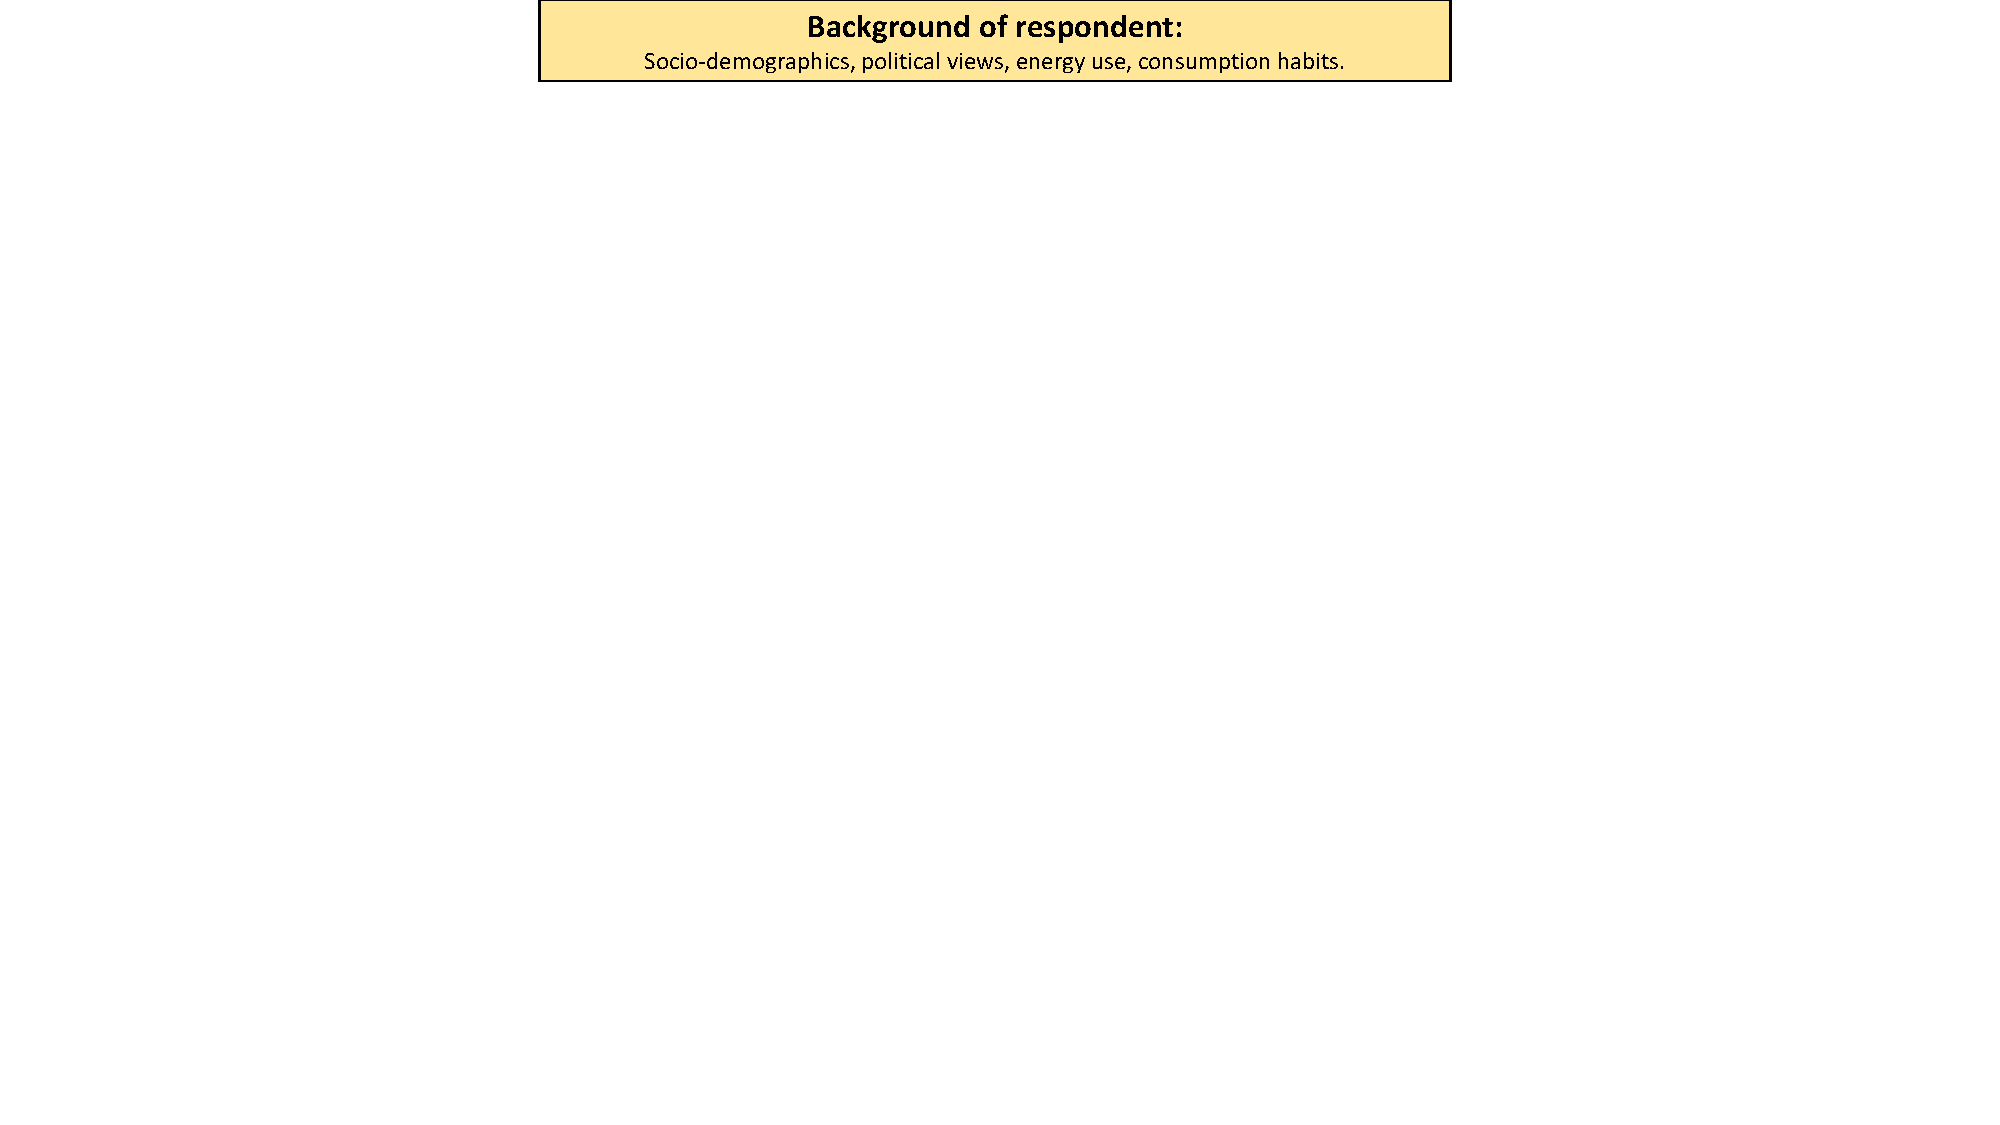
\includegraphics[width=.9\textwidth]{../figures/survey_flow/survey_flow_new-1.pdf}}}
\only<+>{\makebox[\textwidth][c]{ 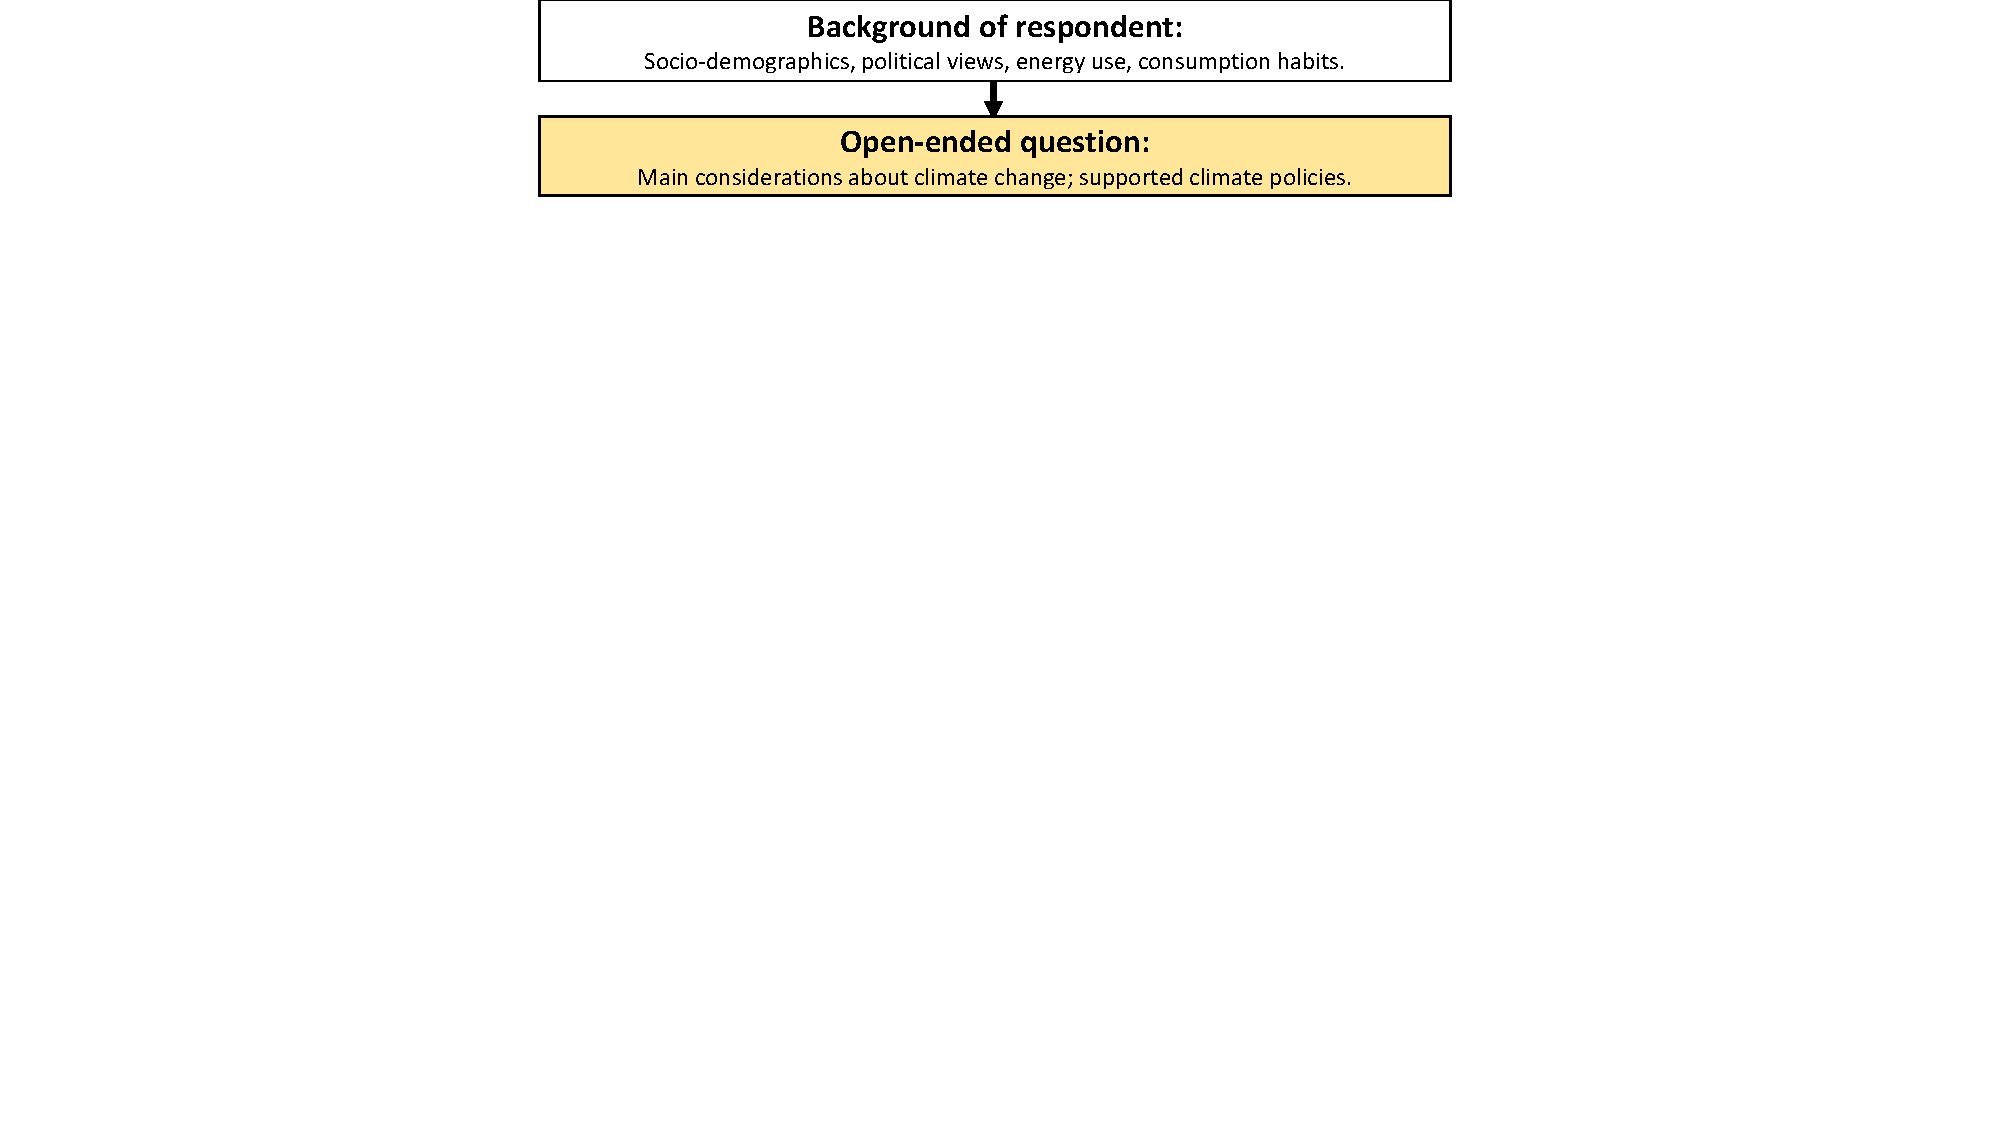
\includegraphics[width=.9\textwidth]{../figures/survey_flow/survey_flow_new-2.pdf}}}
\only<+>{\makebox[\textwidth][c]{ 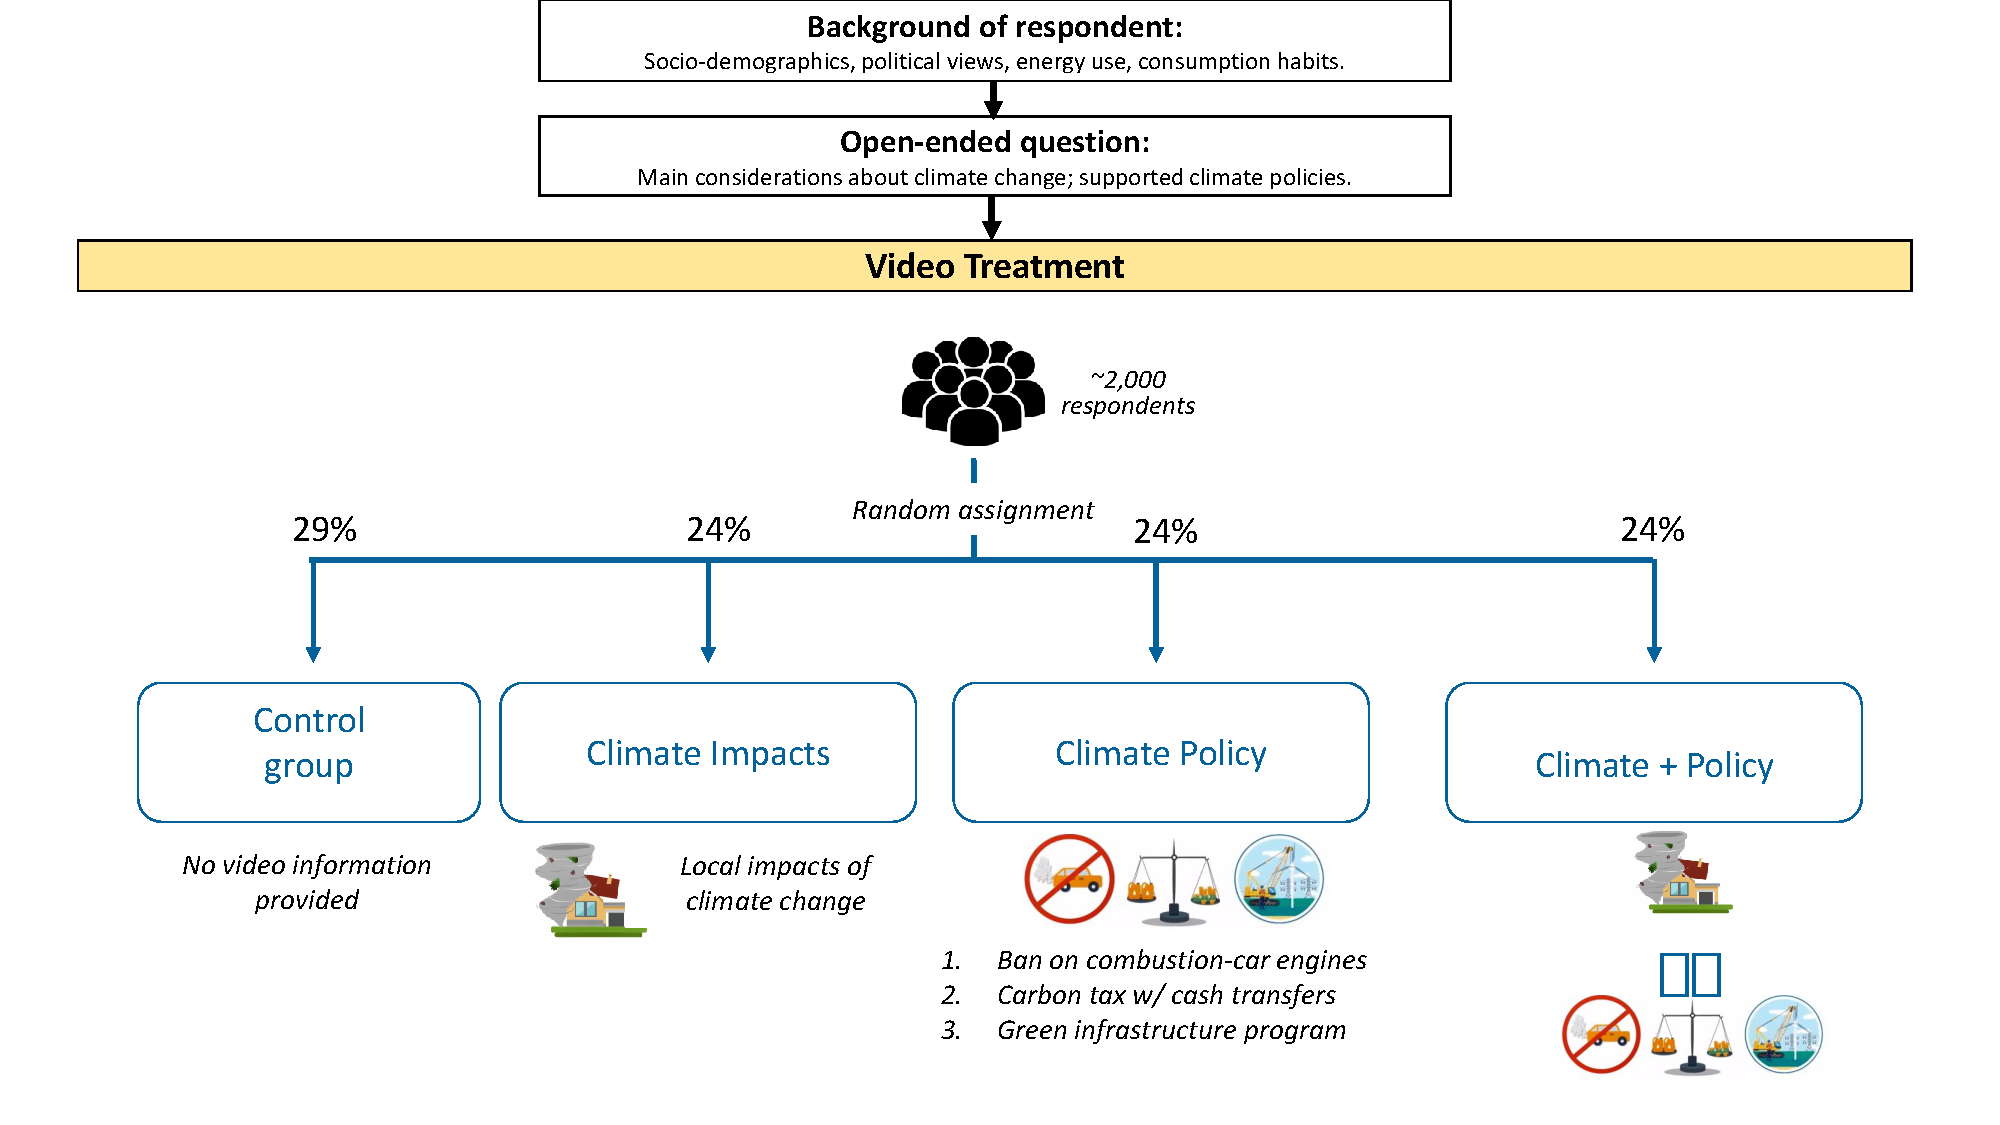
\includegraphics[width=.9\textwidth]{../figures/survey_flow/survey_flow_new-3.pdf}}}
\only<+>{\makebox[\textwidth][c]{ 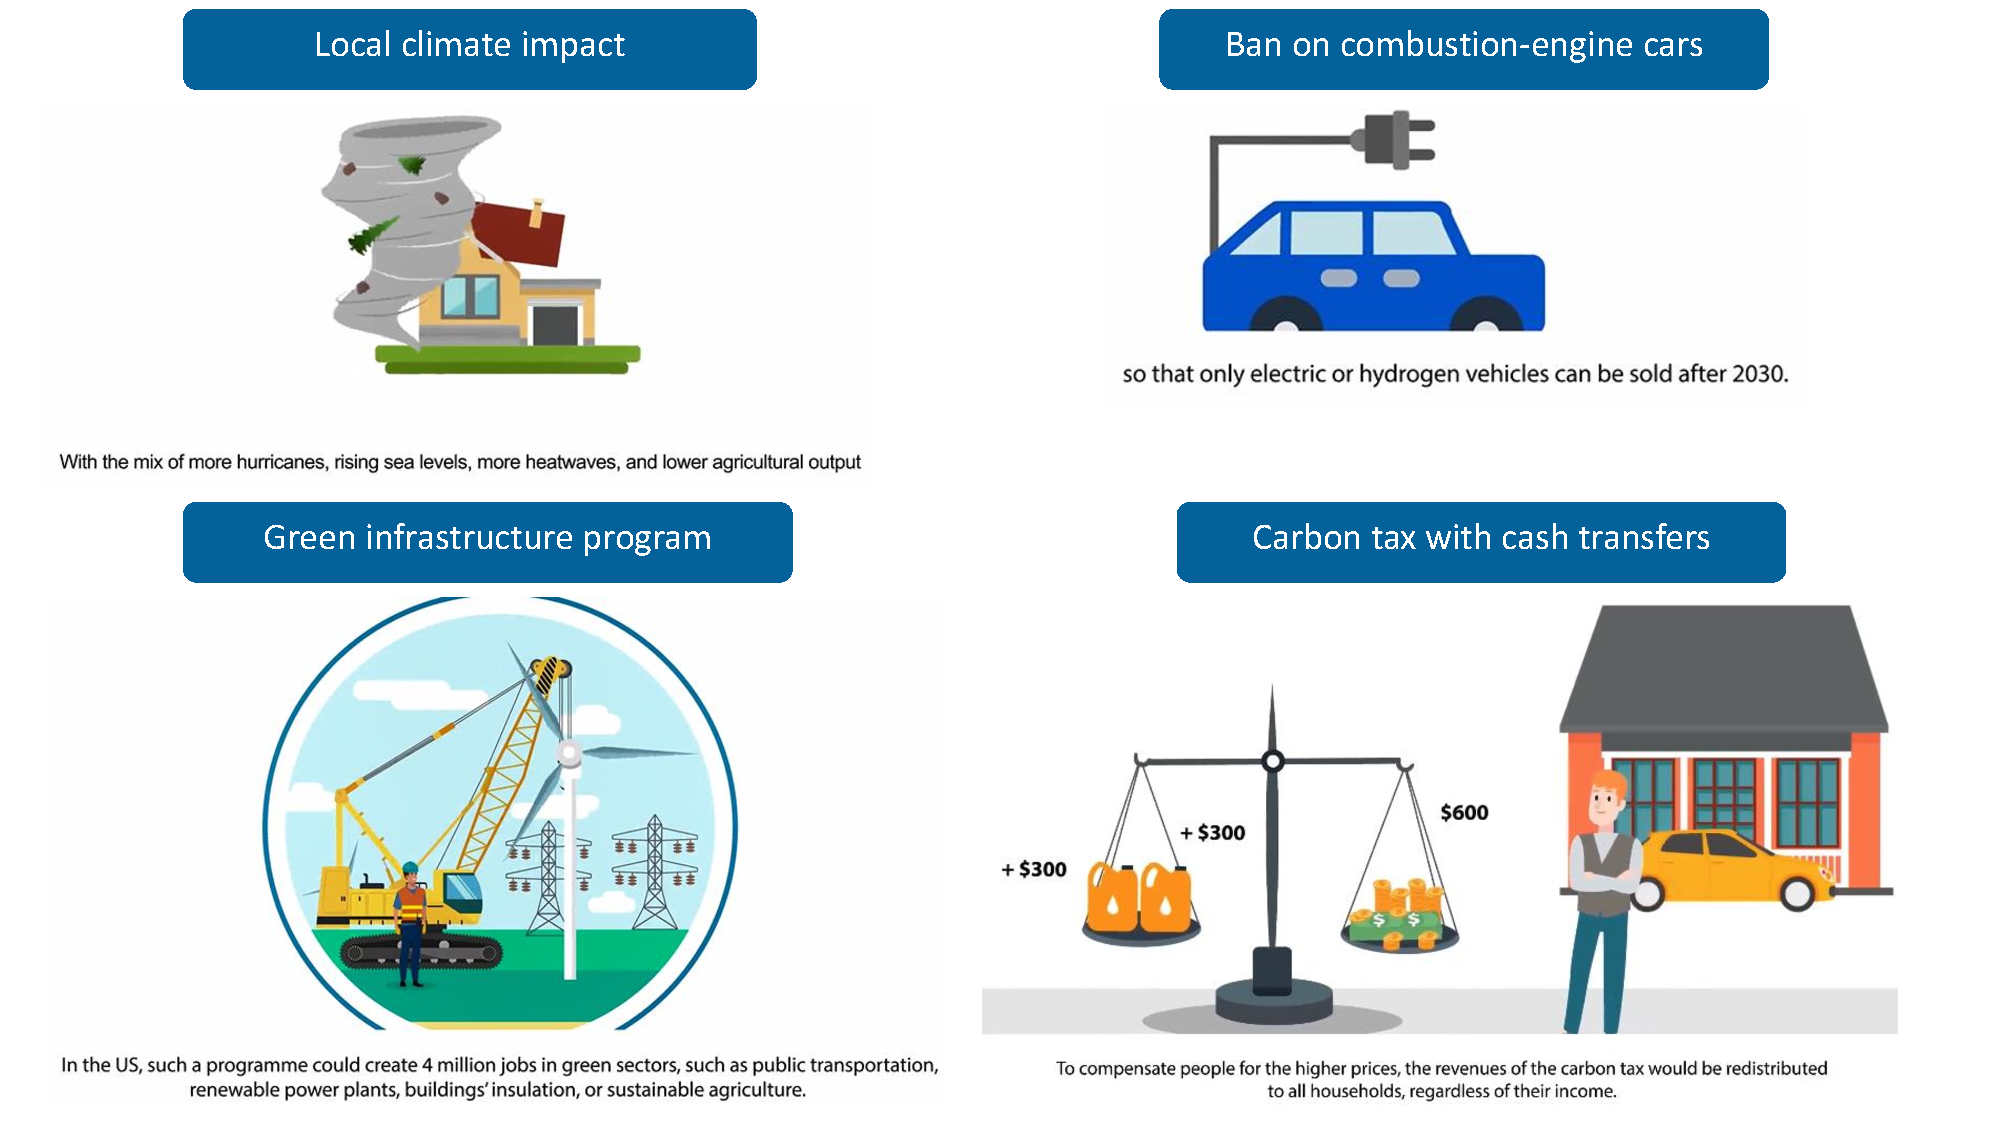
\includegraphics[width=.9\textwidth]{../figures/survey_flow/survey_flow_new-4.pdf}}}
\only<+>{\makebox[\textwidth][c]{ 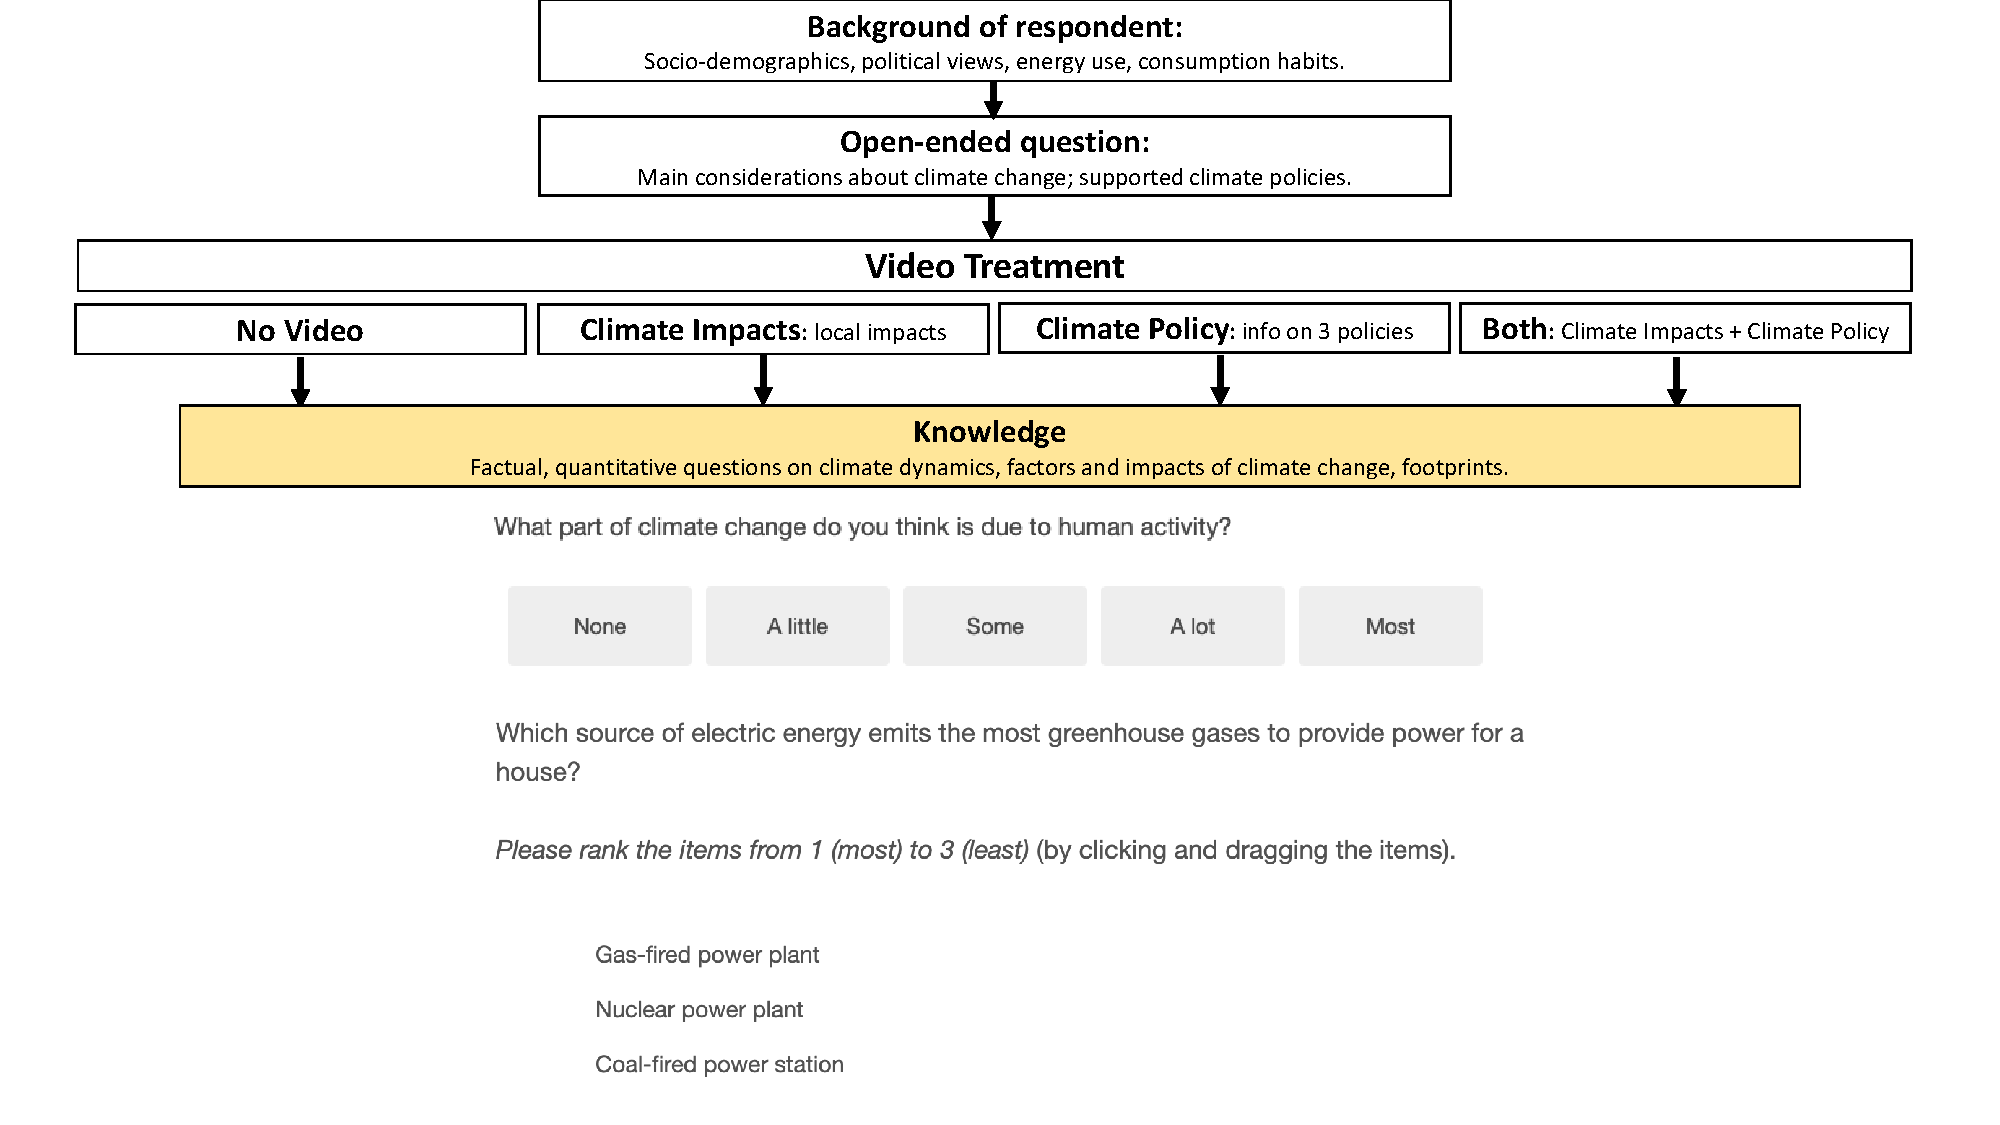
\includegraphics[width=.9\textwidth]{../figures/survey_flow/survey_flow_new-5.pdf}}}
\only<+>{\makebox[\textwidth][c]{ 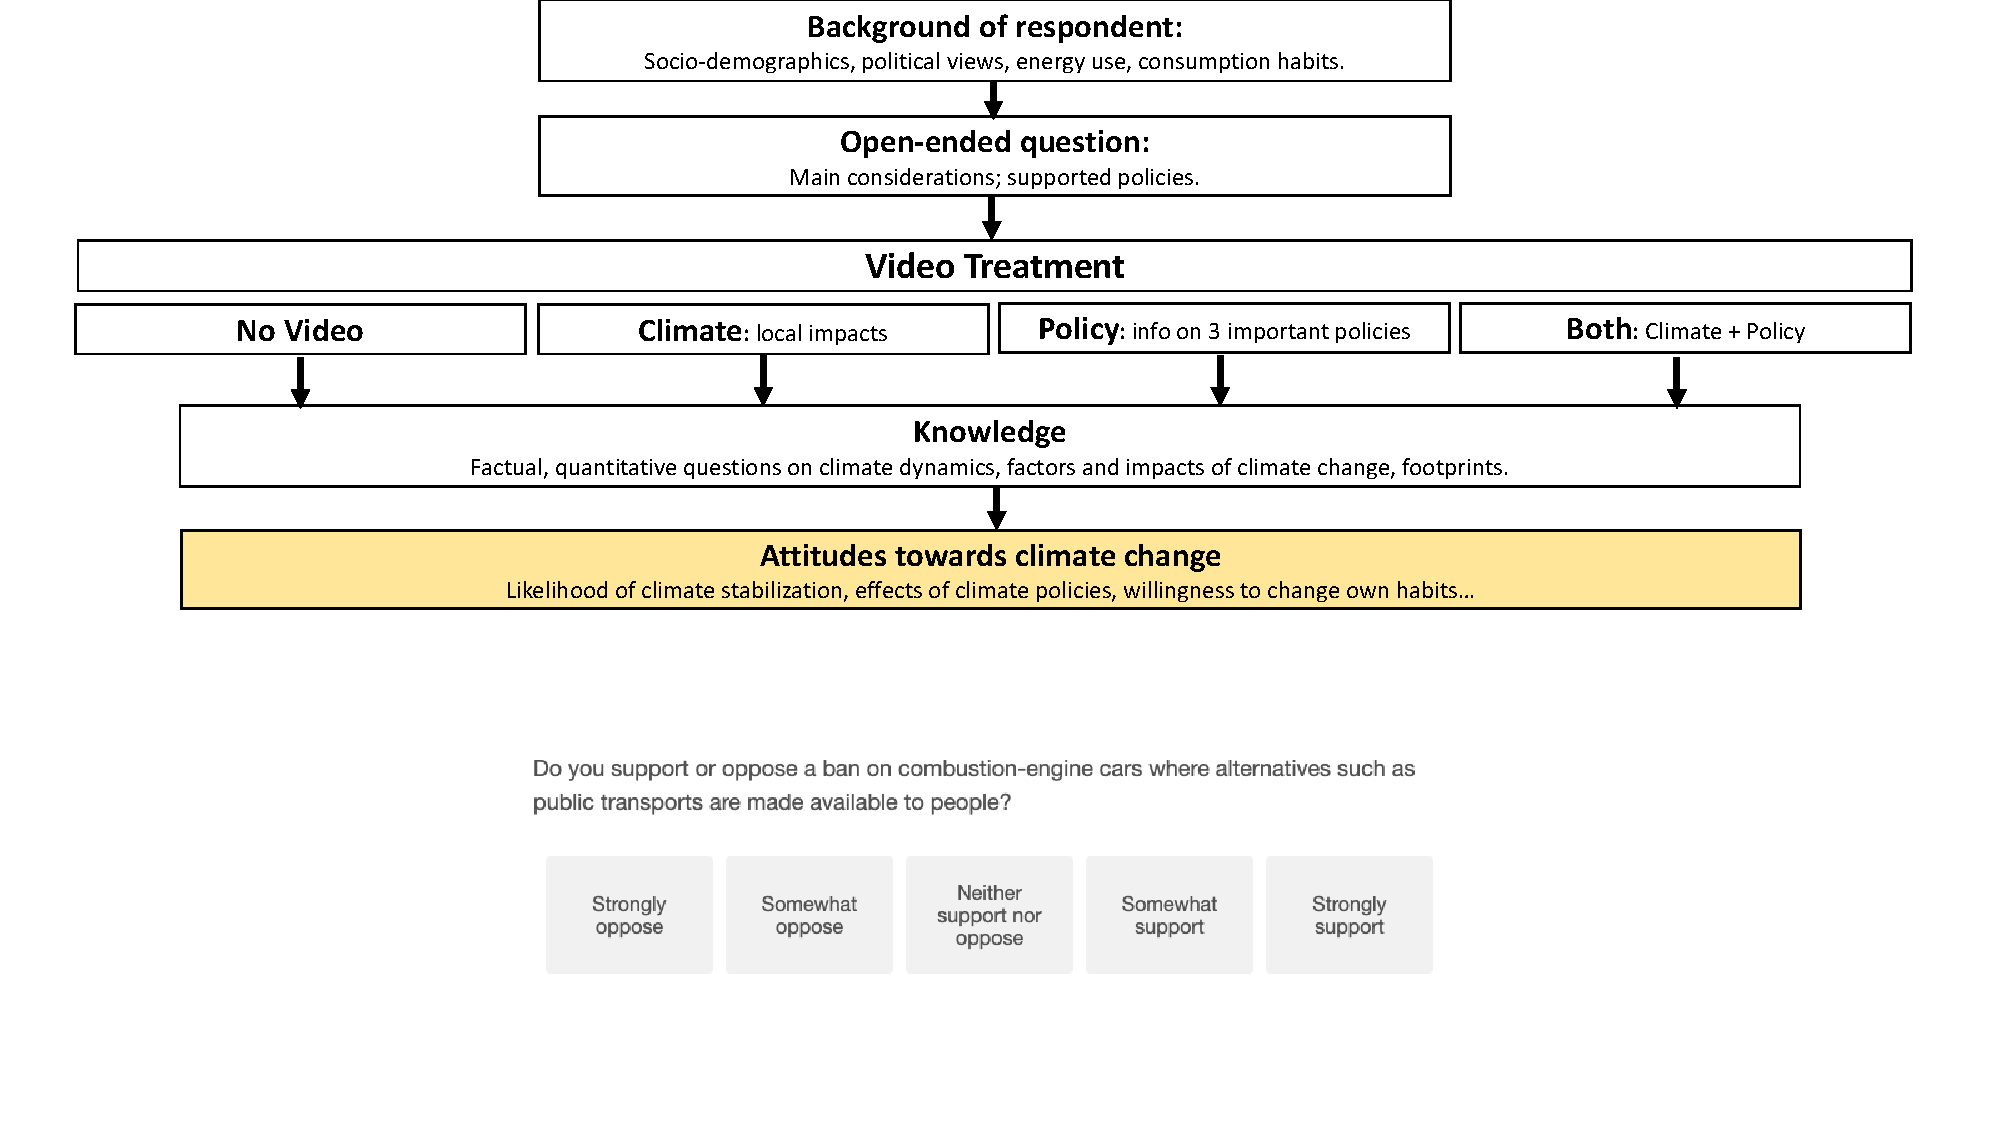
\includegraphics[width=.9\textwidth]{../figures/survey_flow/survey_flow_new-6.pdf}}}
\only<+>{\makebox[\textwidth][c]{ 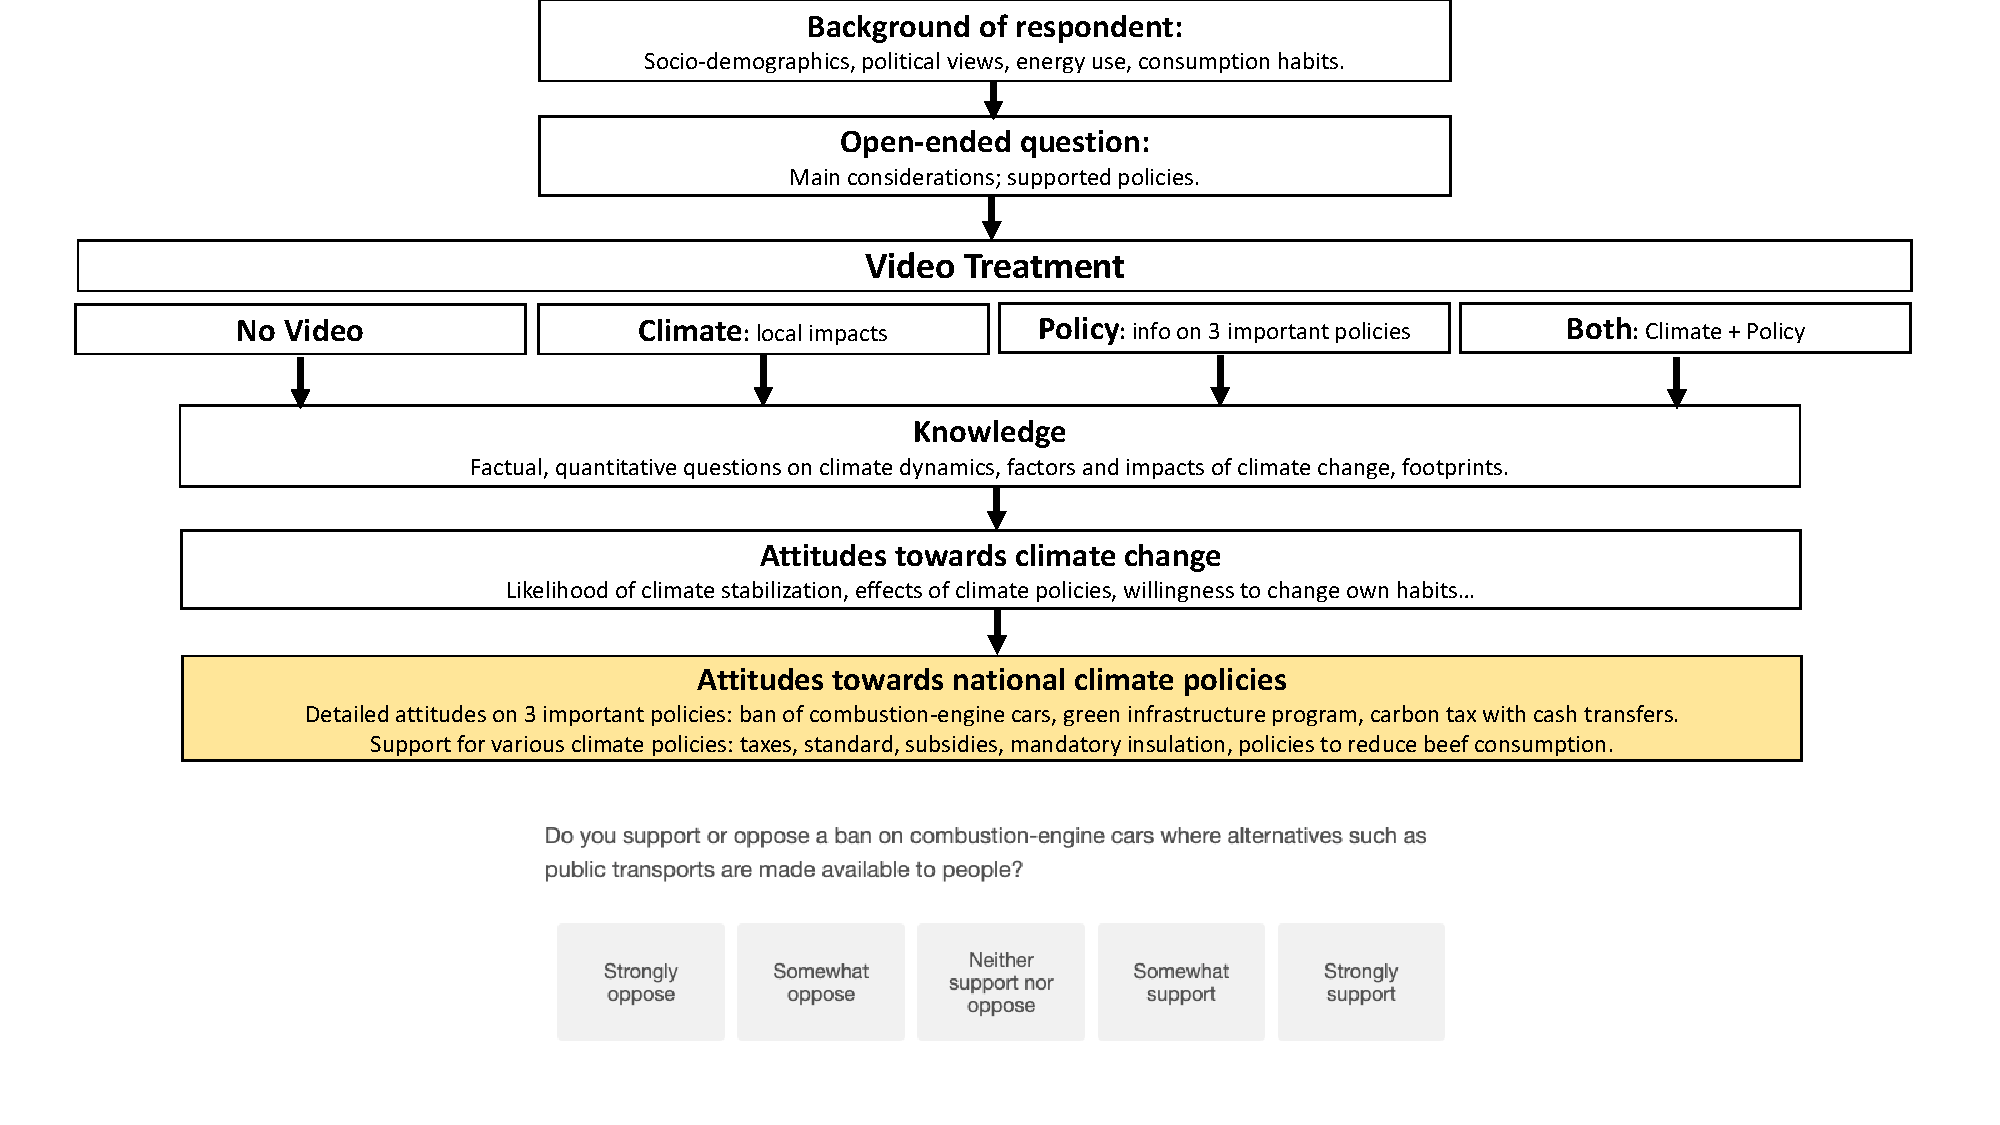
\includegraphics[width=.9\textwidth]{../figures/survey_flow/survey_flow_new-7.pdf}}}
\only<+>{\makebox[\textwidth][c]{ 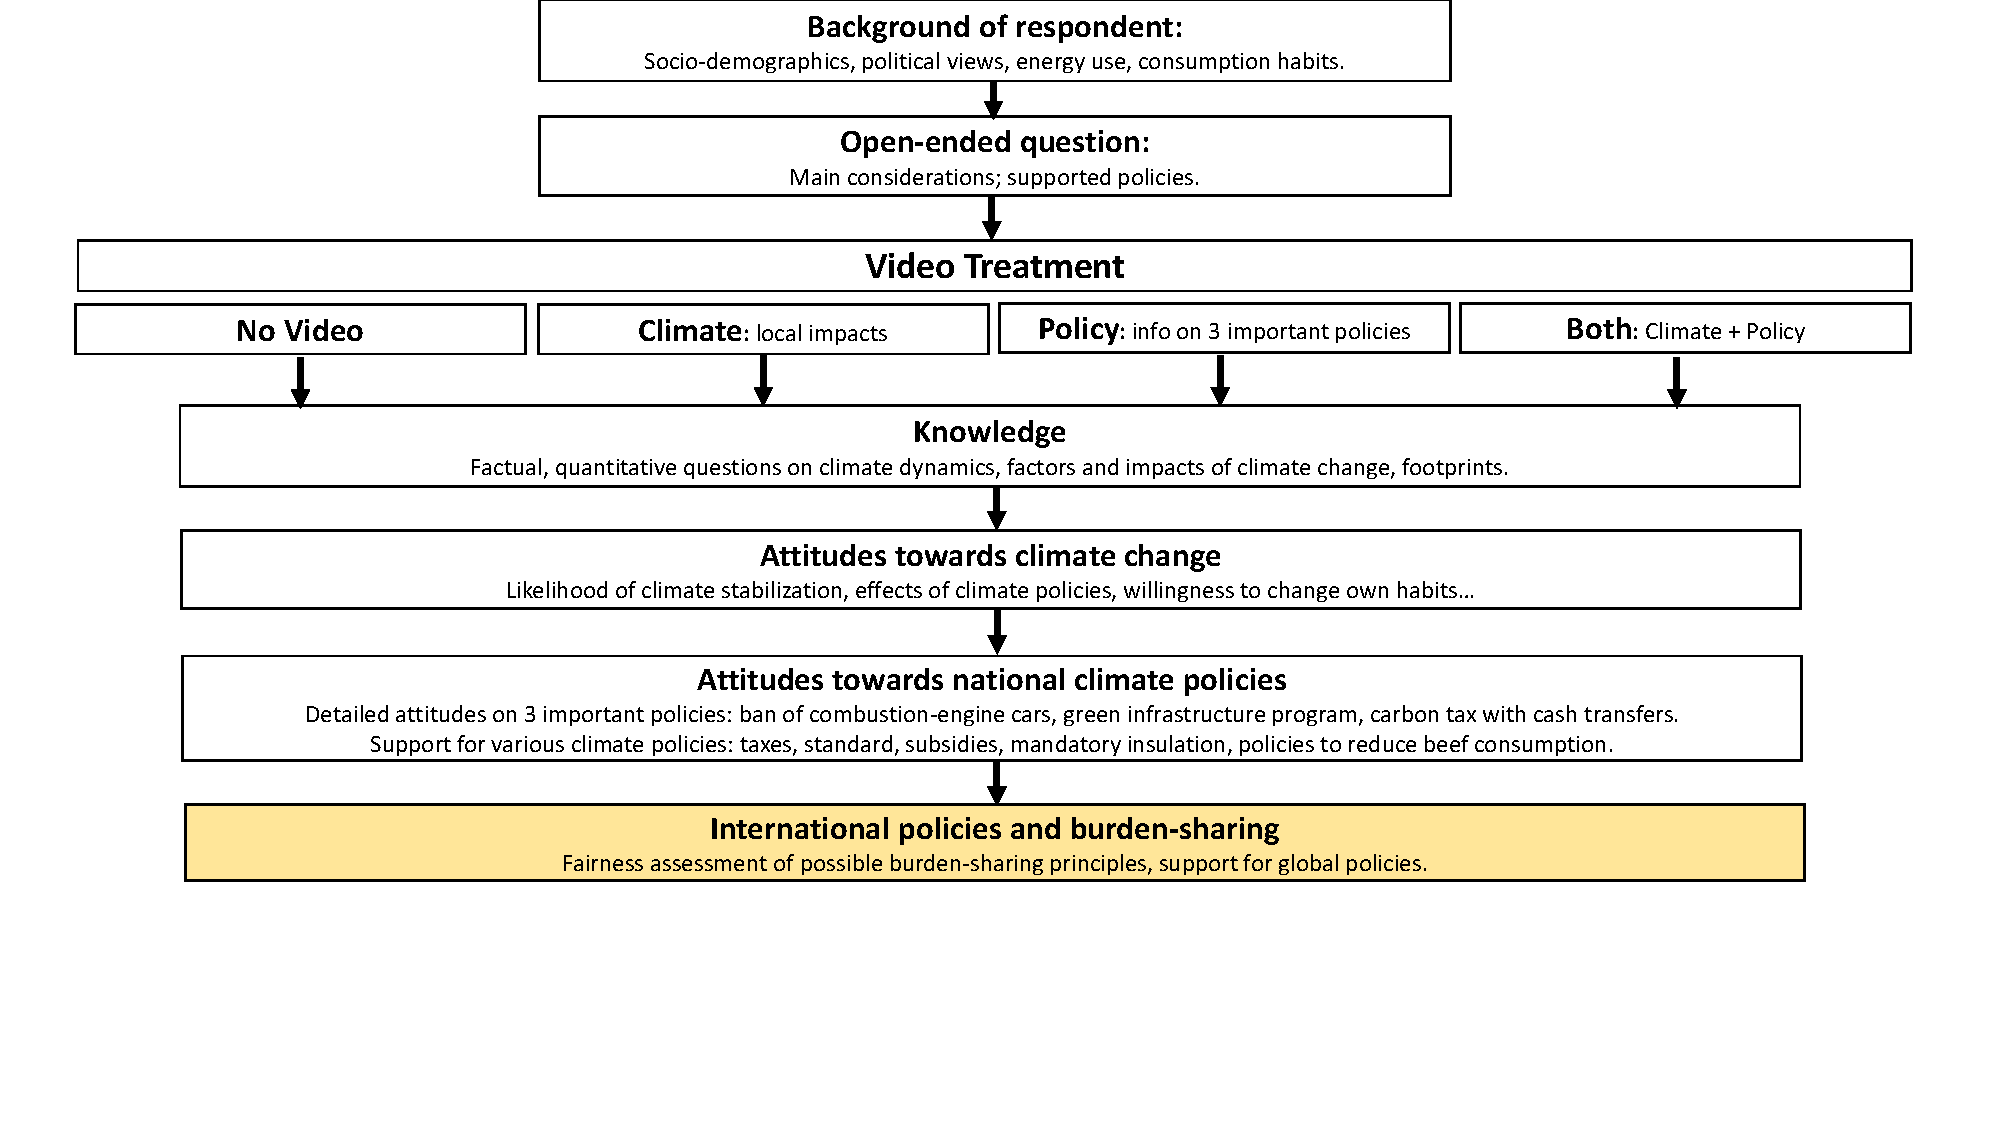
\includegraphics[width=.9\textwidth]{../figures/survey_flow/survey_flow_new-8.pdf}}}
\only<+>{\makebox[\textwidth][c]{ 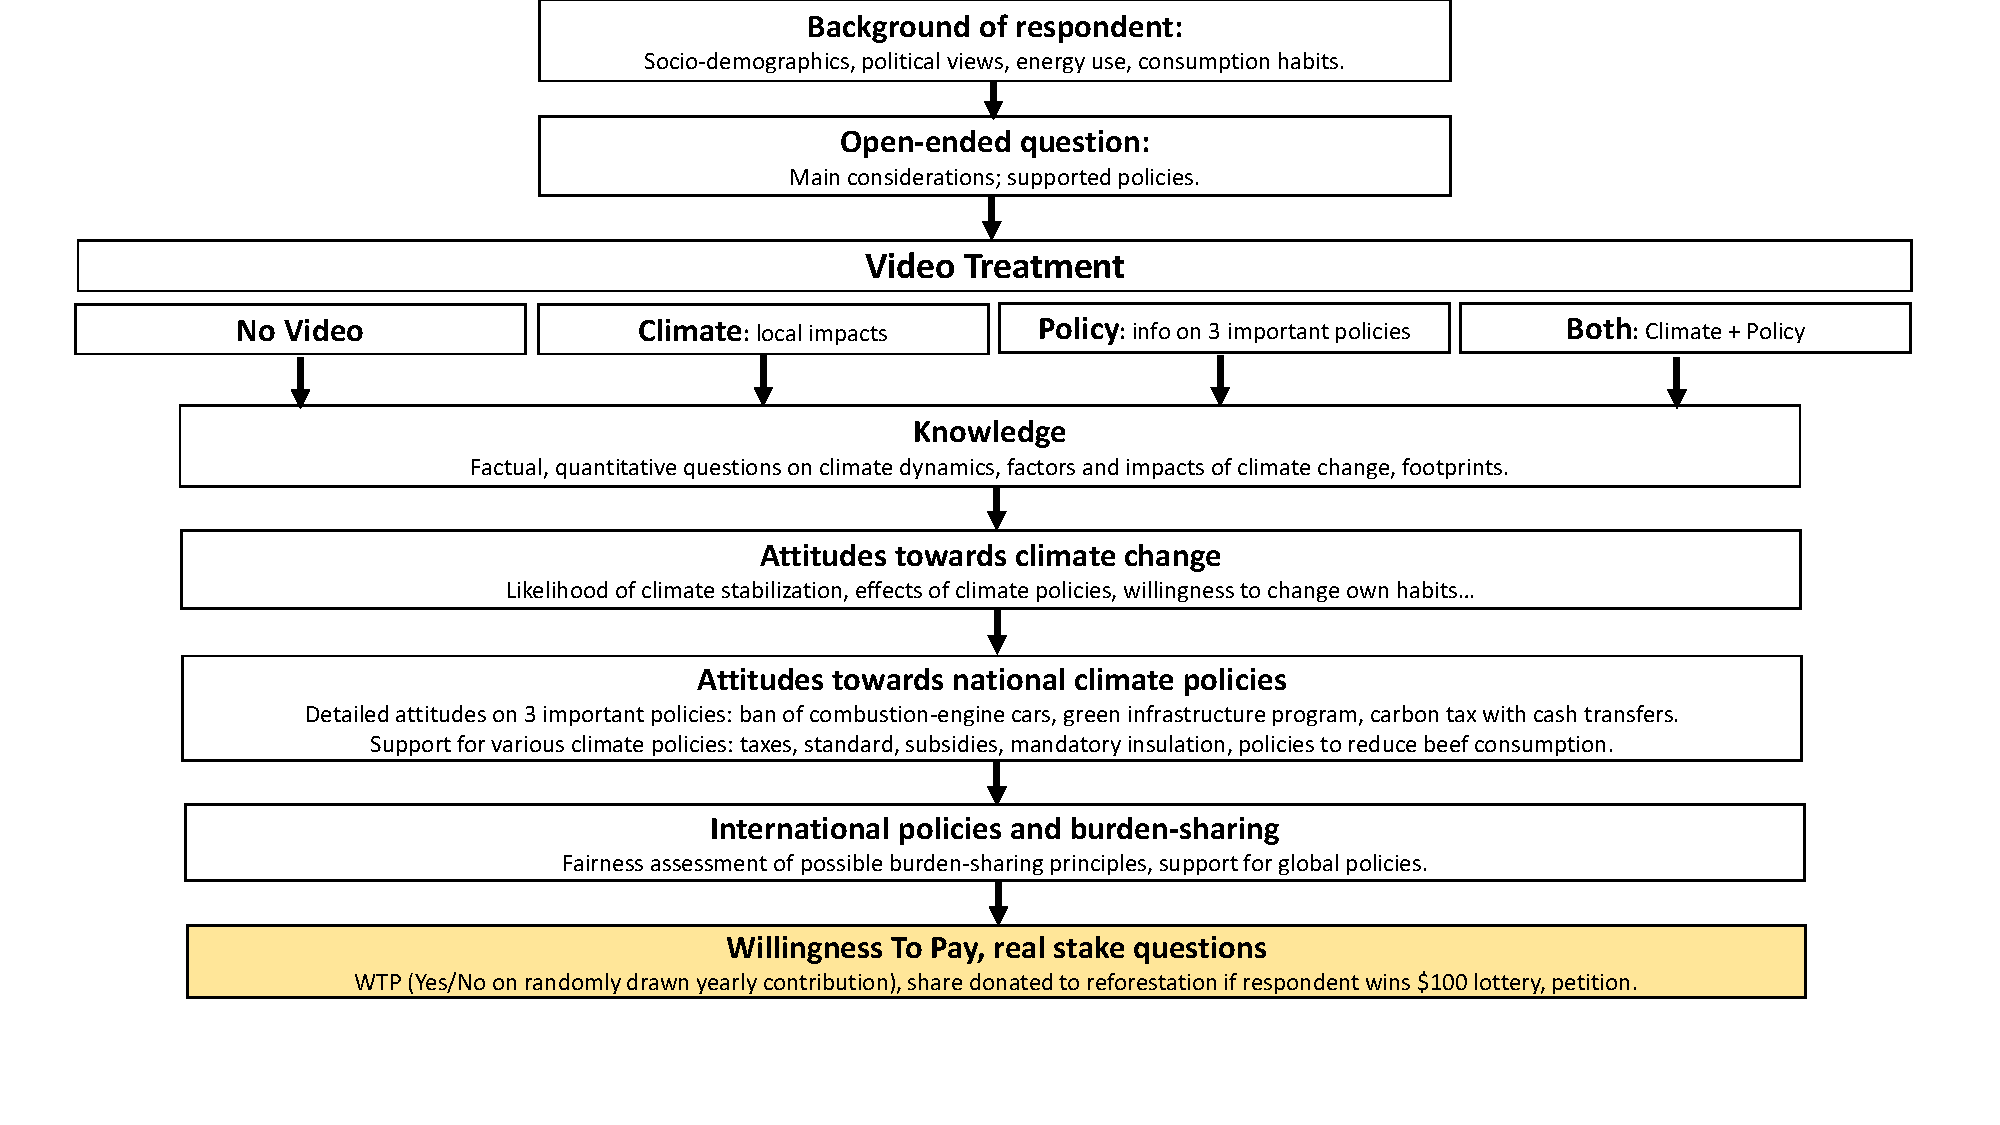
\includegraphics[width=.9\textwidth]{../figures/survey_flow/survey_flow_new-9.pdf}}}
\only<+>{\makebox[\textwidth][c]{ 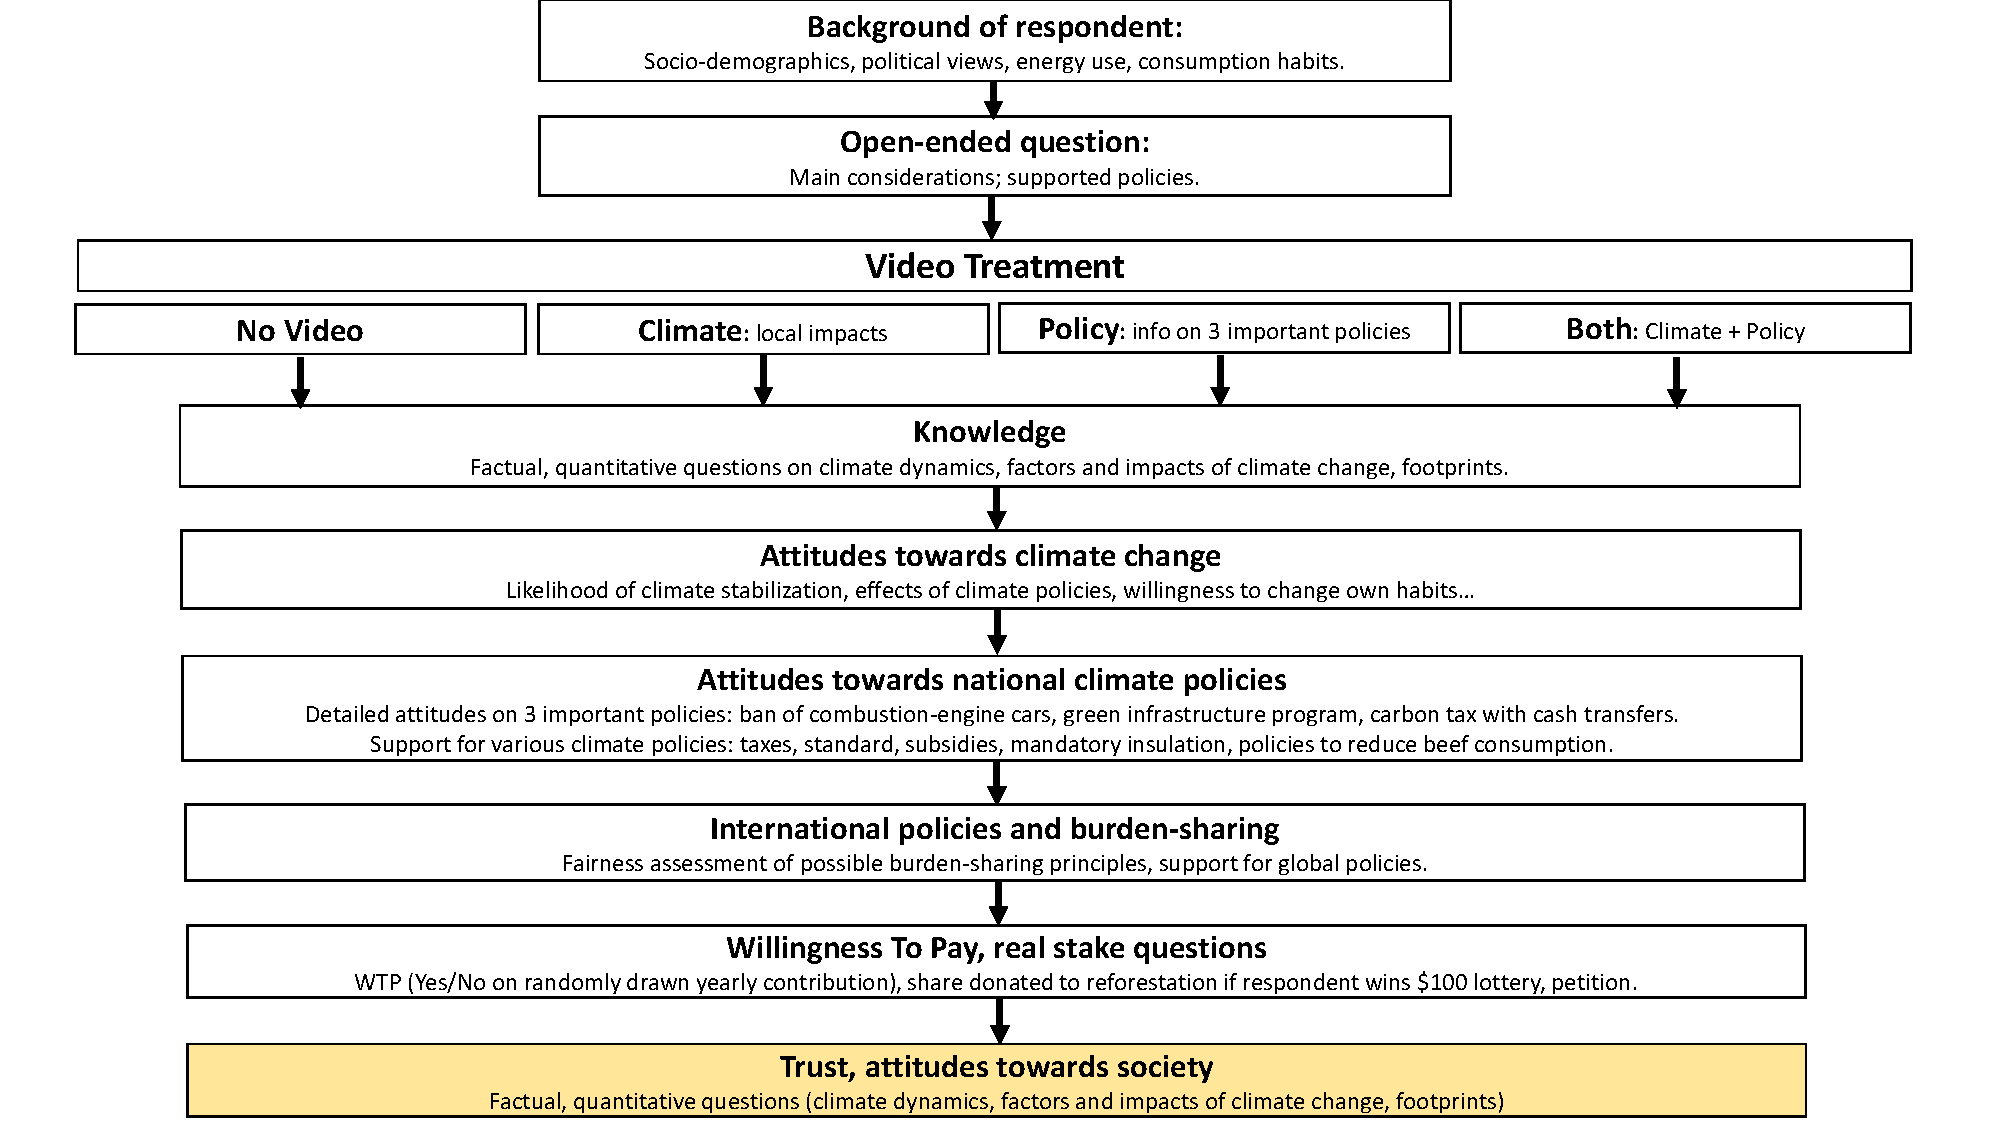
\includegraphics[width=.9\textwidth]{../figures/survey_flow/survey_flow_new-10.pdf}}}
\only<+>{\makebox[\textwidth][c]{ 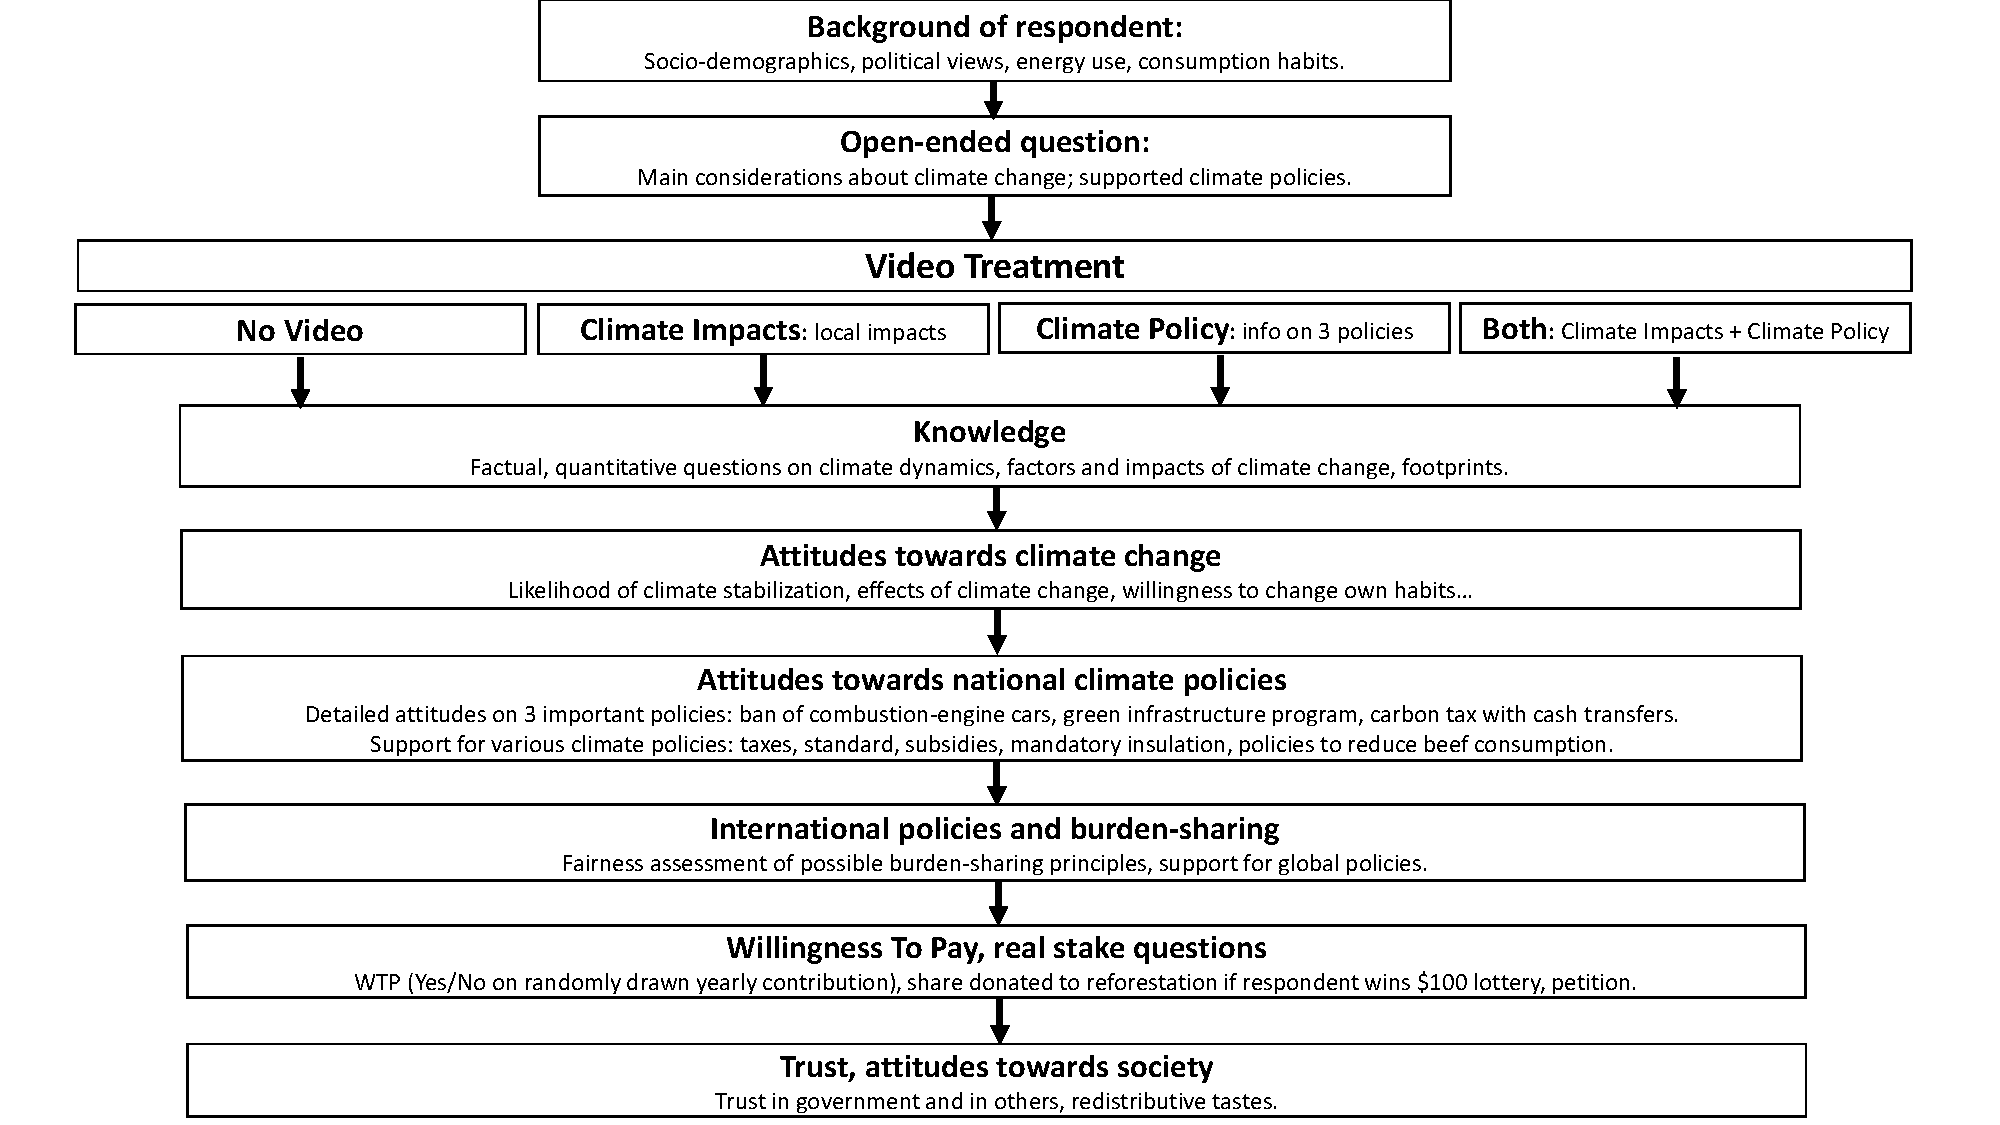
\includegraphics[width=.9\textwidth]{../figures/survey_flow/survey_flow_new-11.pdf}}}
%\end{itemize}
%}
\end{frame}

\begin{frame}{Video screenshots}
\vspace{.2cm}
%\makebox[\textwidth][c]{
%\begin{itemize}[<+>]
\only<+>{\makebox[\textwidth][c]{ 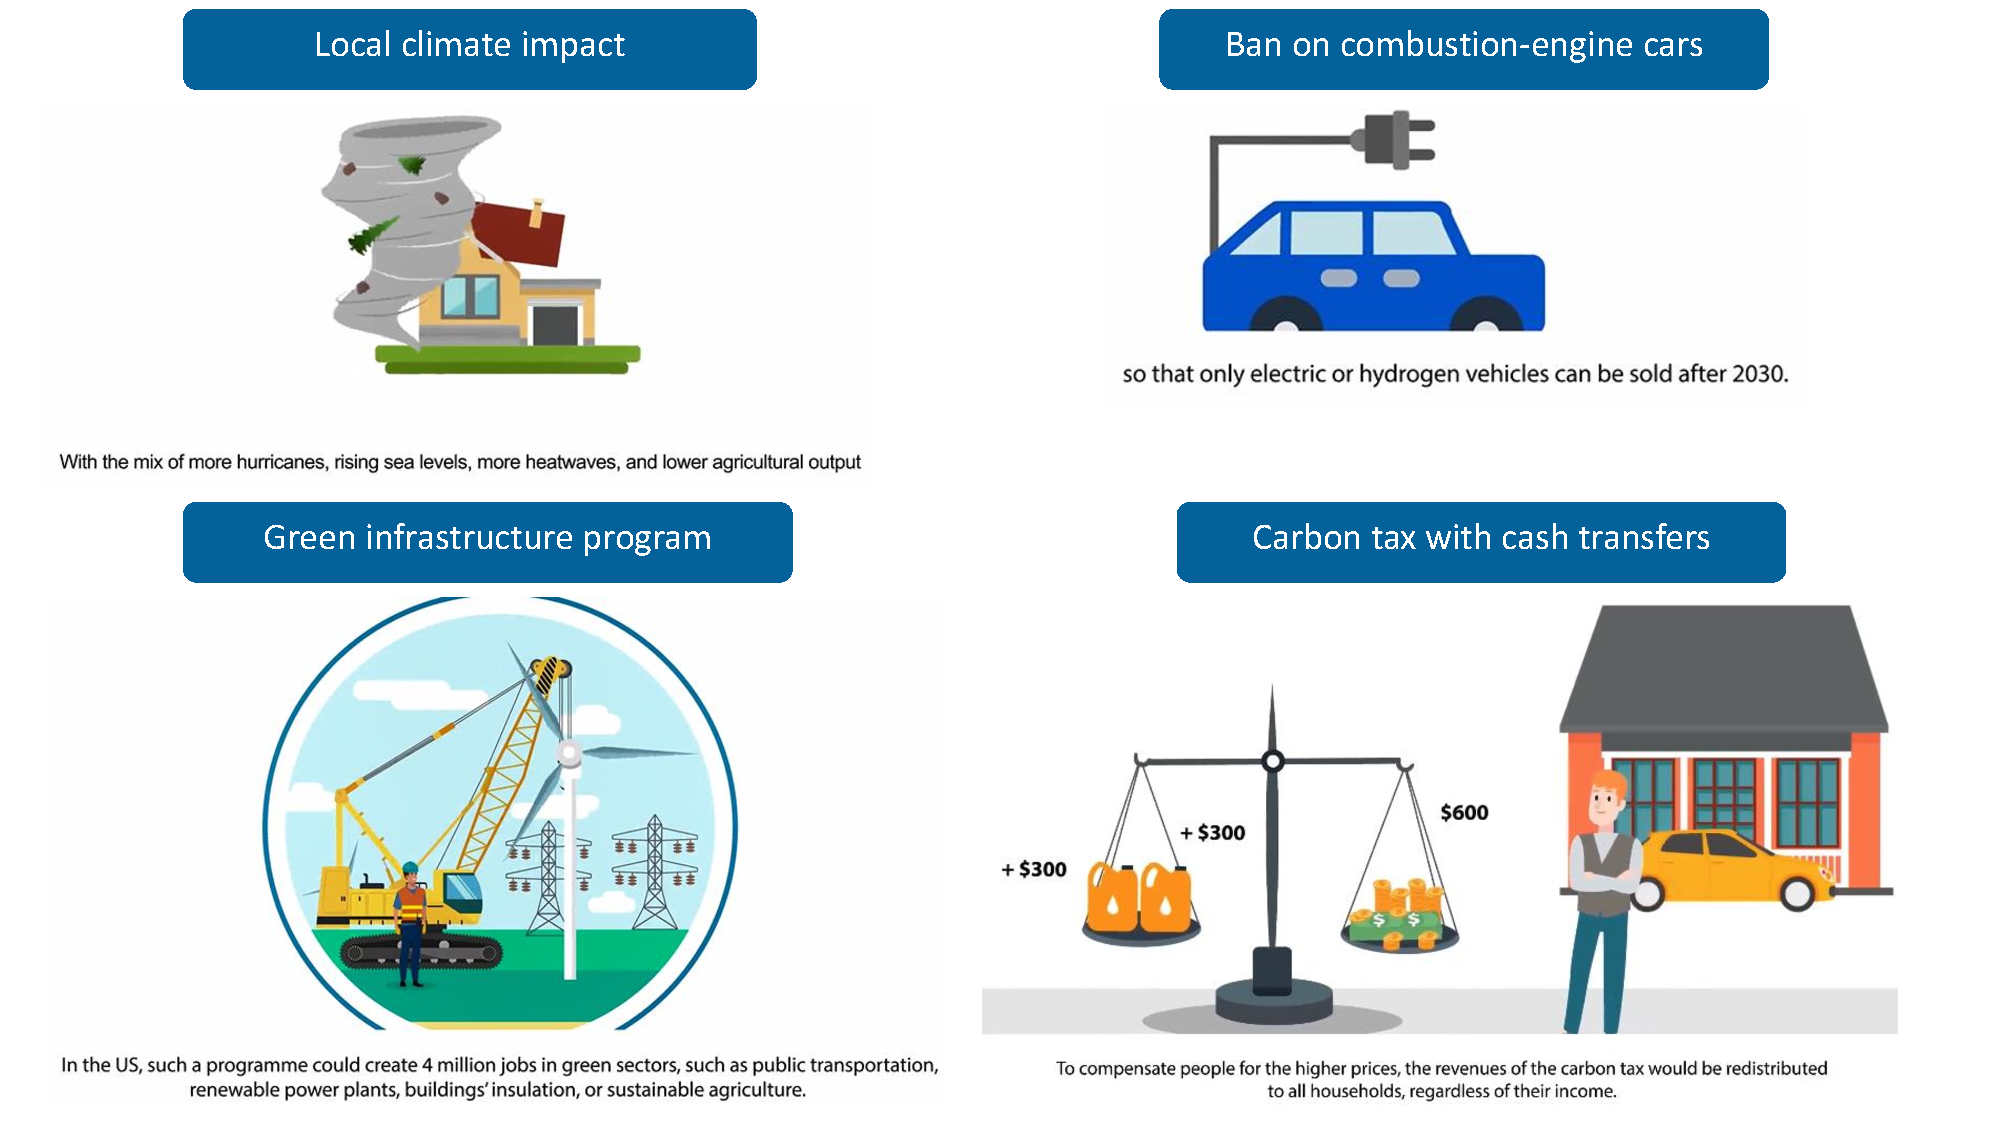
\includegraphics[width=.9\textwidth]{../figures/survey_flow/survey_flow_new-4.pdf}}}
%\end{itemize}
%}
\end{frame}
\begin{frame}{Questionnaire}
\vspace{.2cm}
%\makebox[\textwidth][c]{
%\begin{itemize}[<+>]
\only<+>{\makebox[\textwidth][c]{ 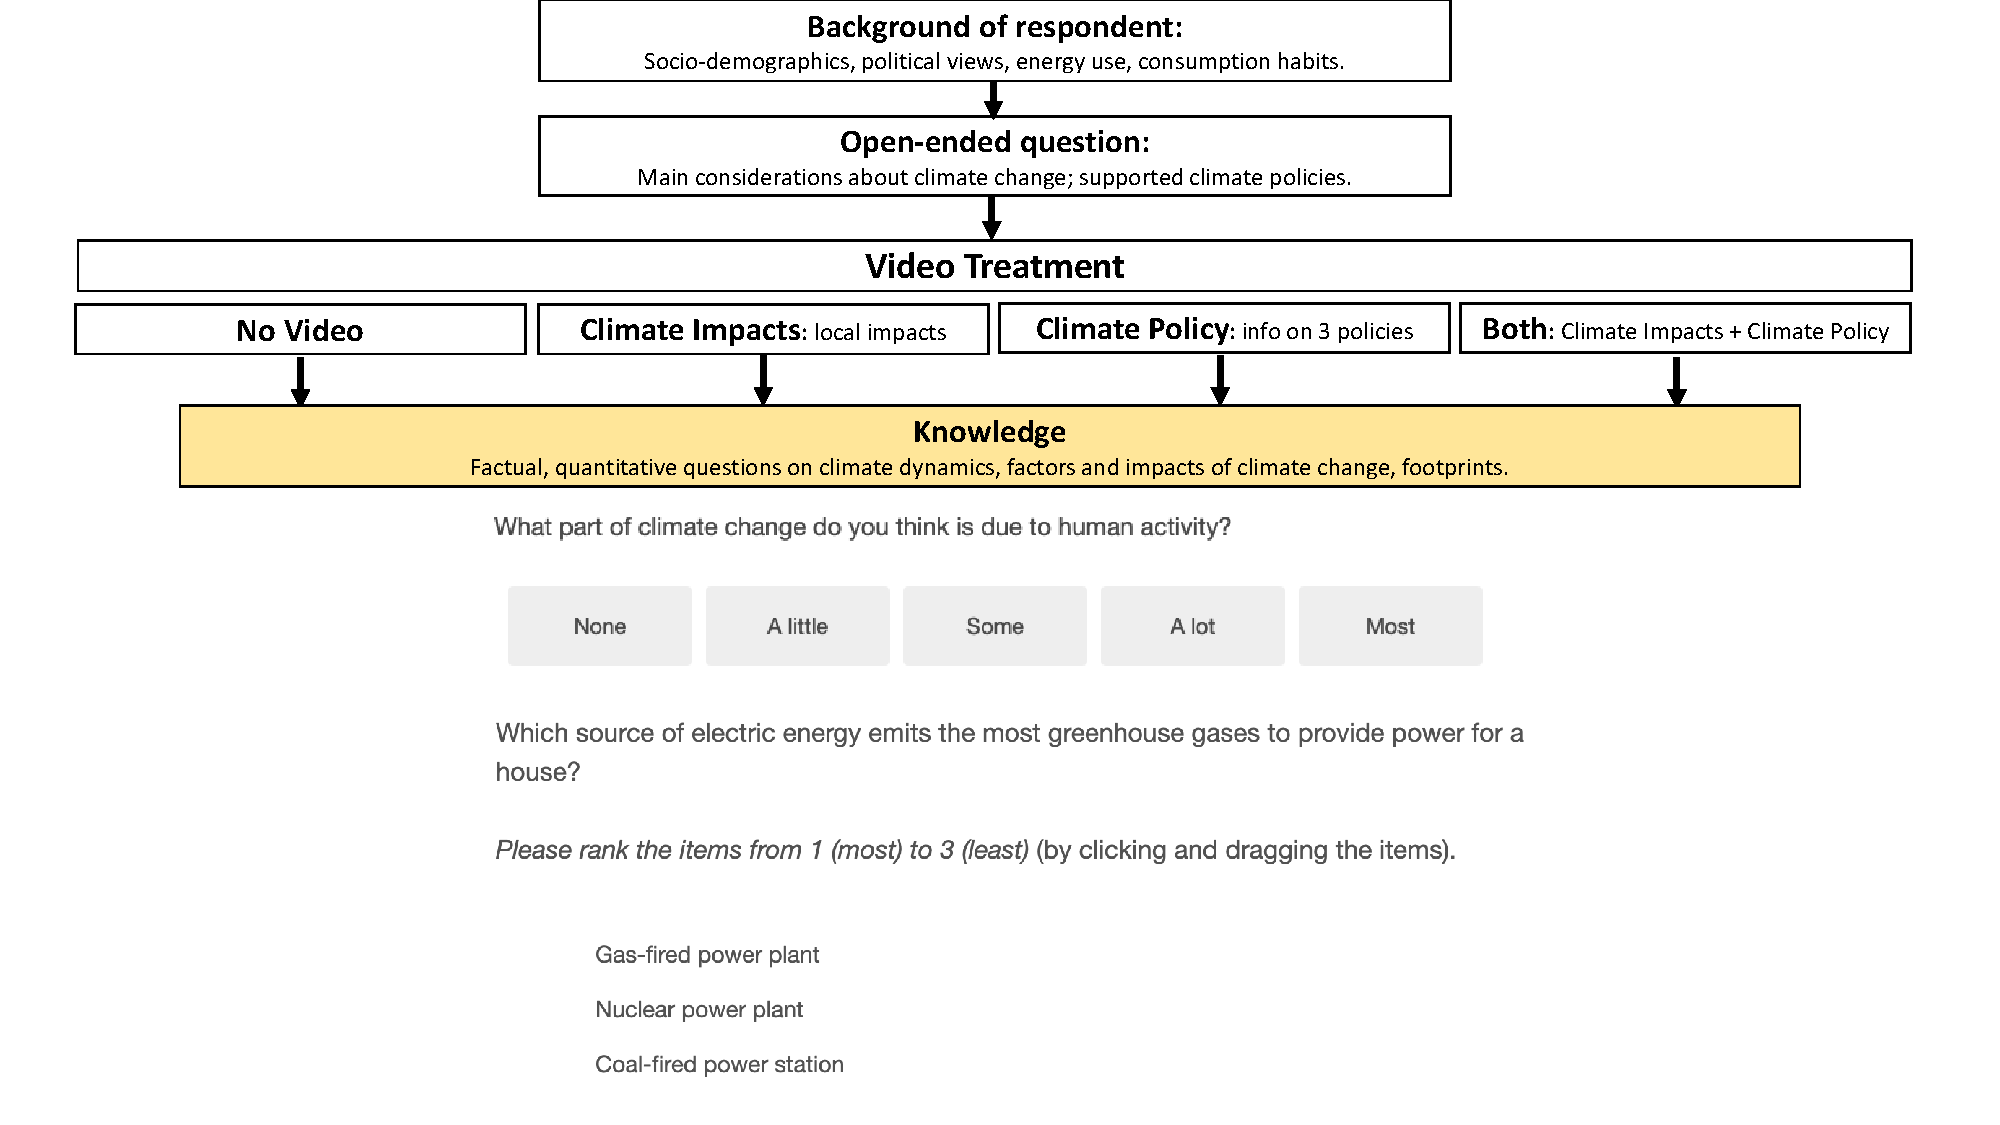
\includegraphics[width=.9\textwidth]{../figures/survey_flow/survey_flow_new-5.pdf}}}
\only<+>{\makebox[\textwidth][c]{ 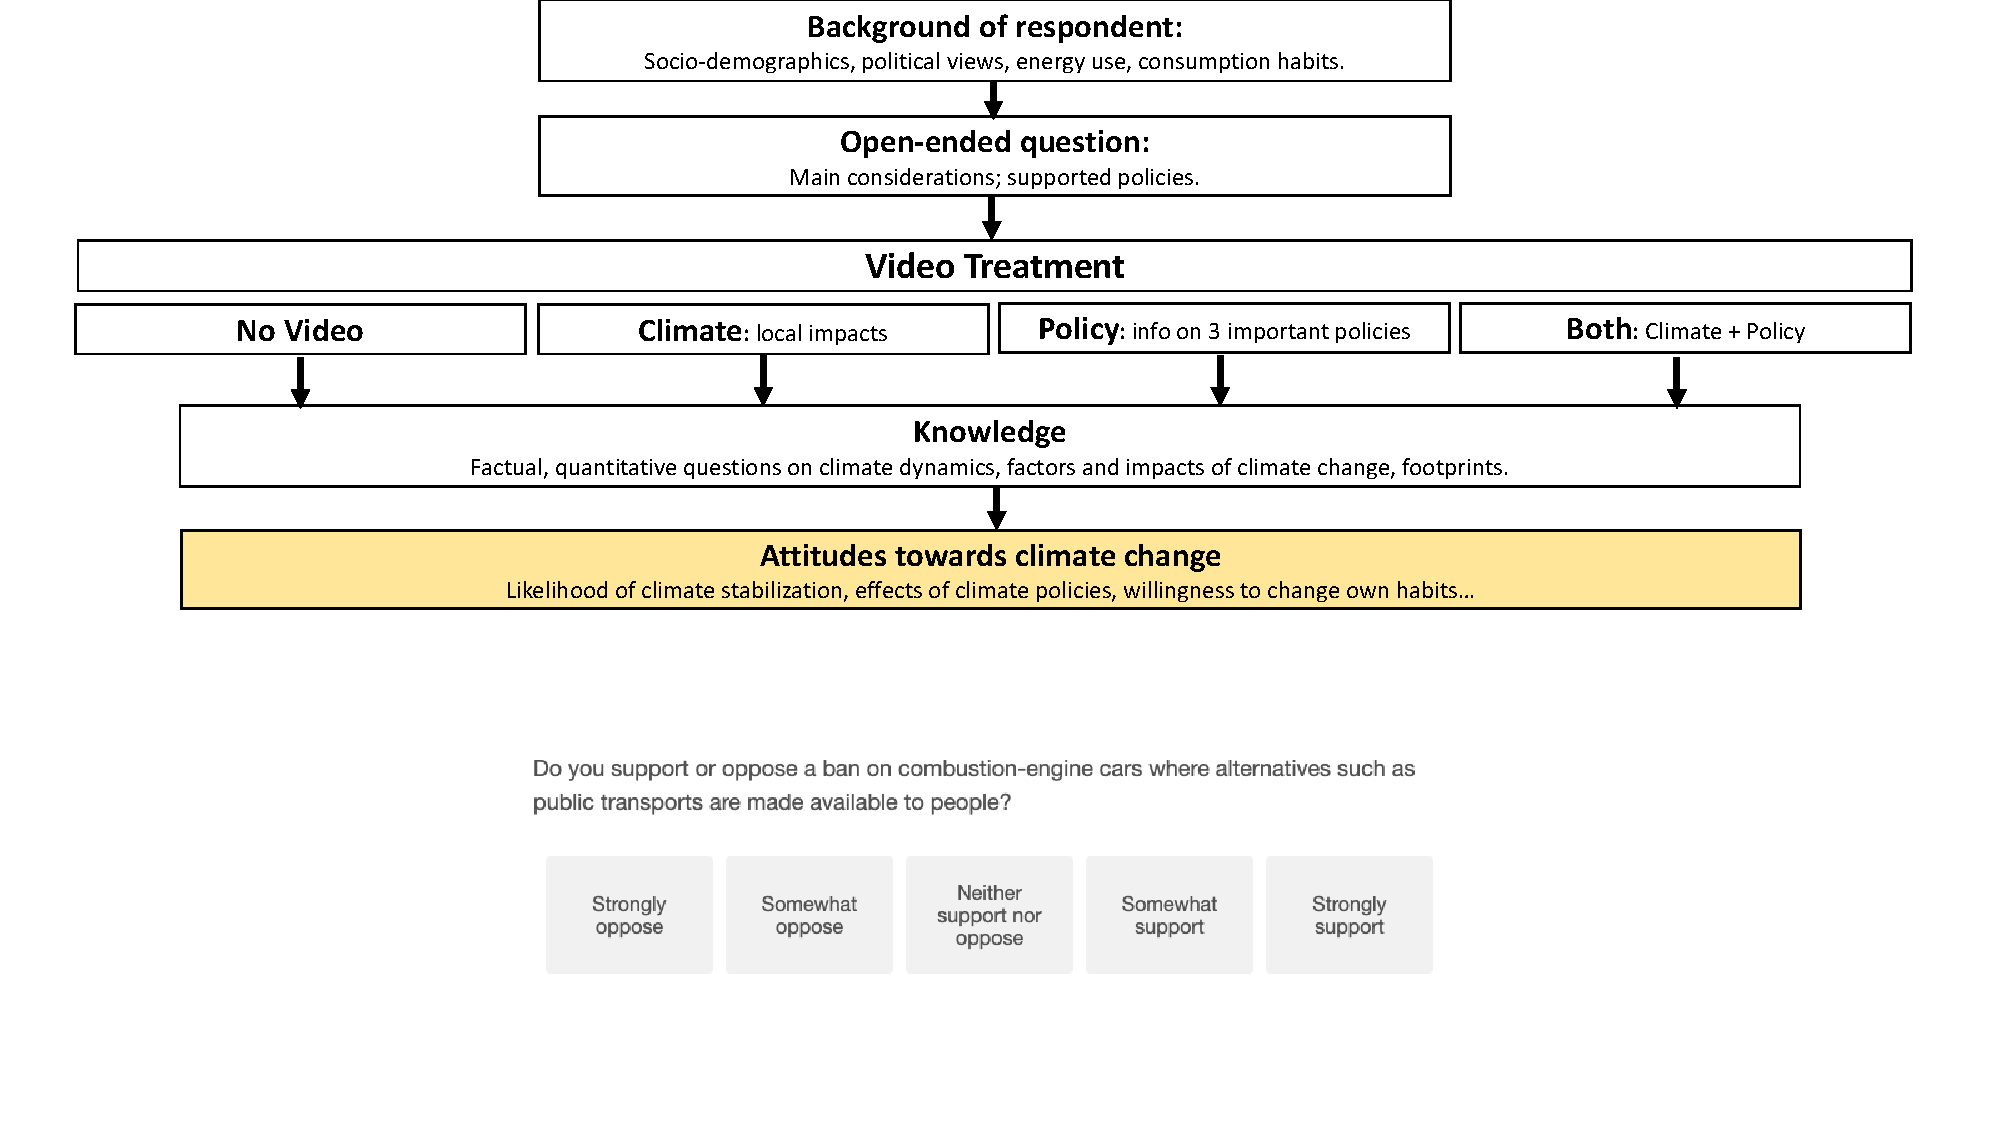
\includegraphics[width=.9\textwidth]{../figures/survey_flow/survey_flow_new-6.pdf}}}
\only<+>{\makebox[\textwidth][c]{ 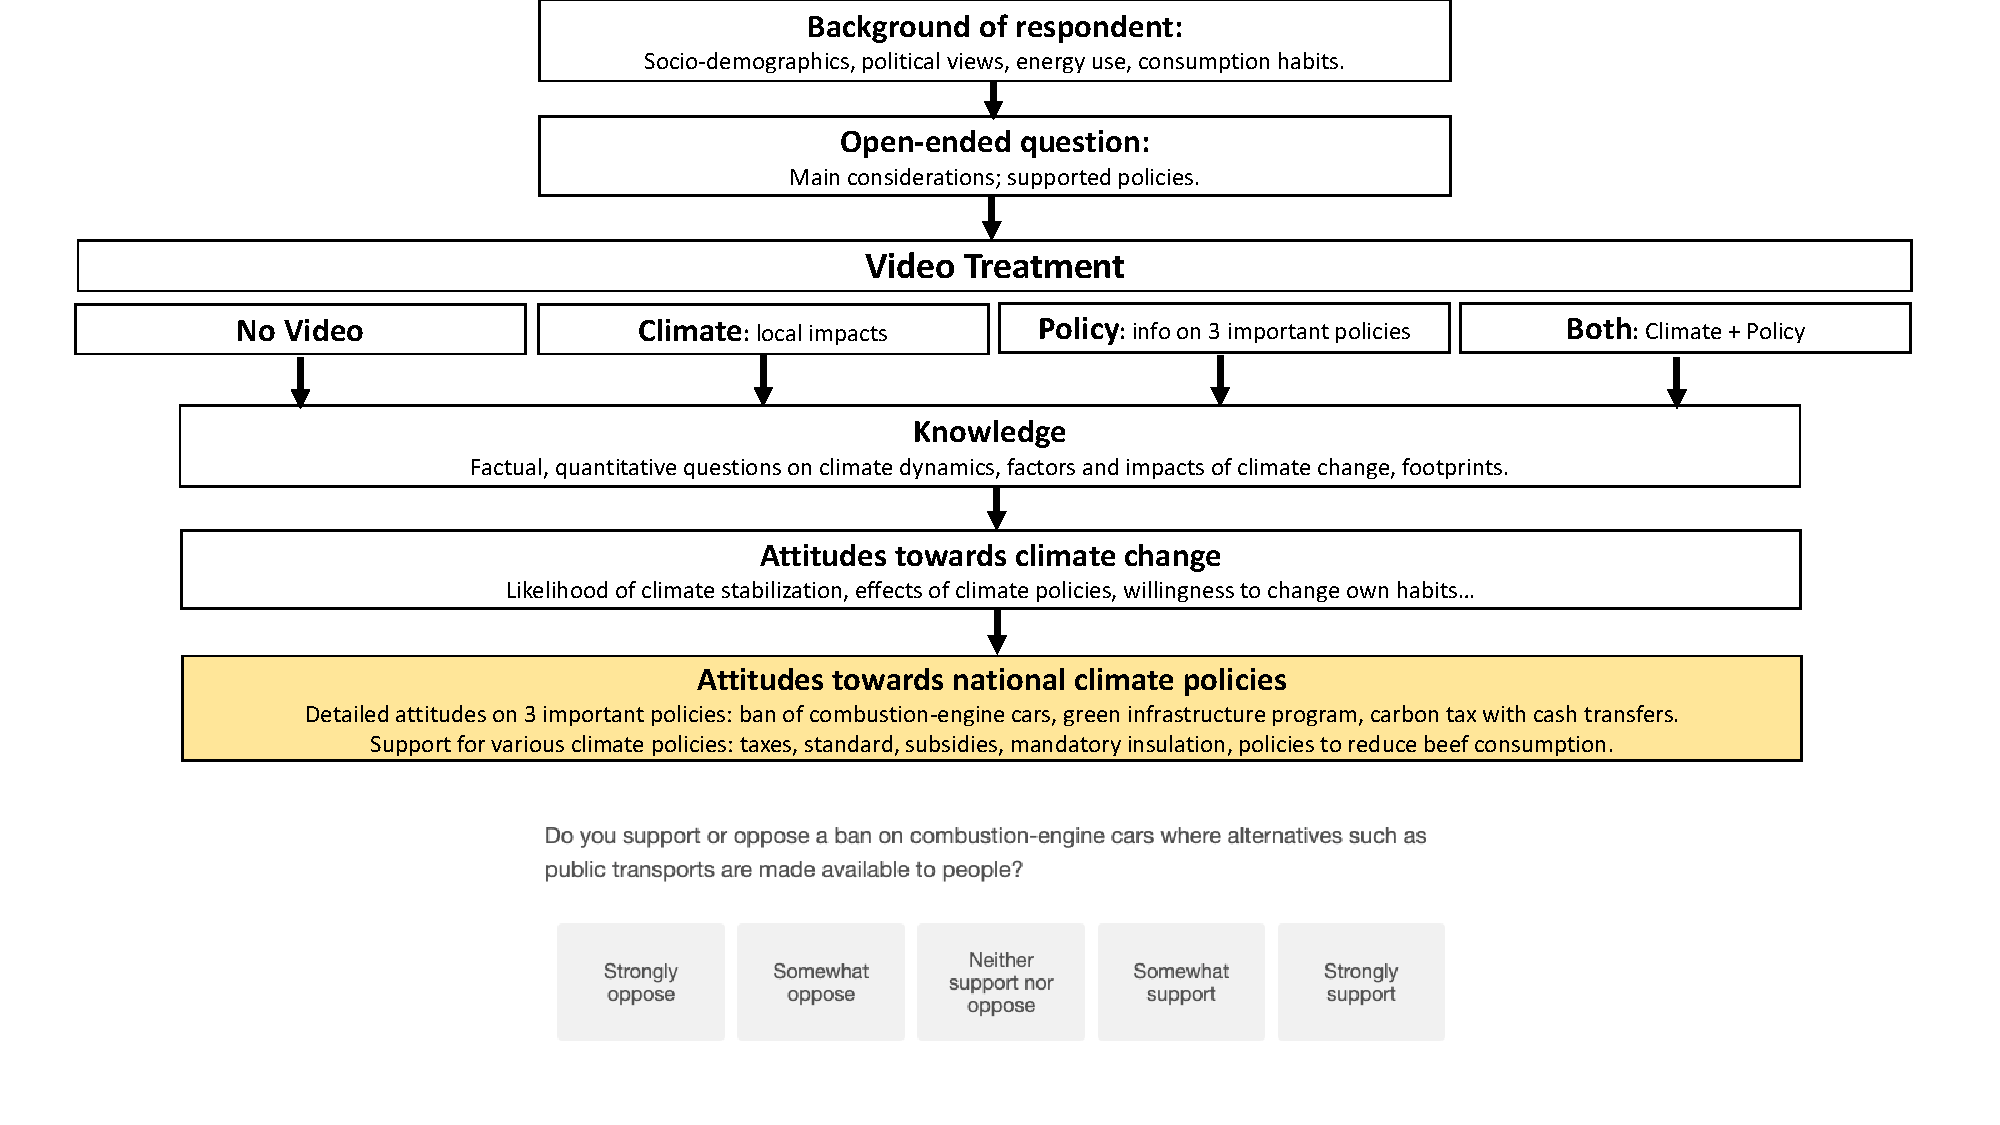
\includegraphics[width=.9\textwidth]{../figures/survey_flow/survey_flow_new-7.pdf}}}
\only<+>{\makebox[\textwidth][c]{ 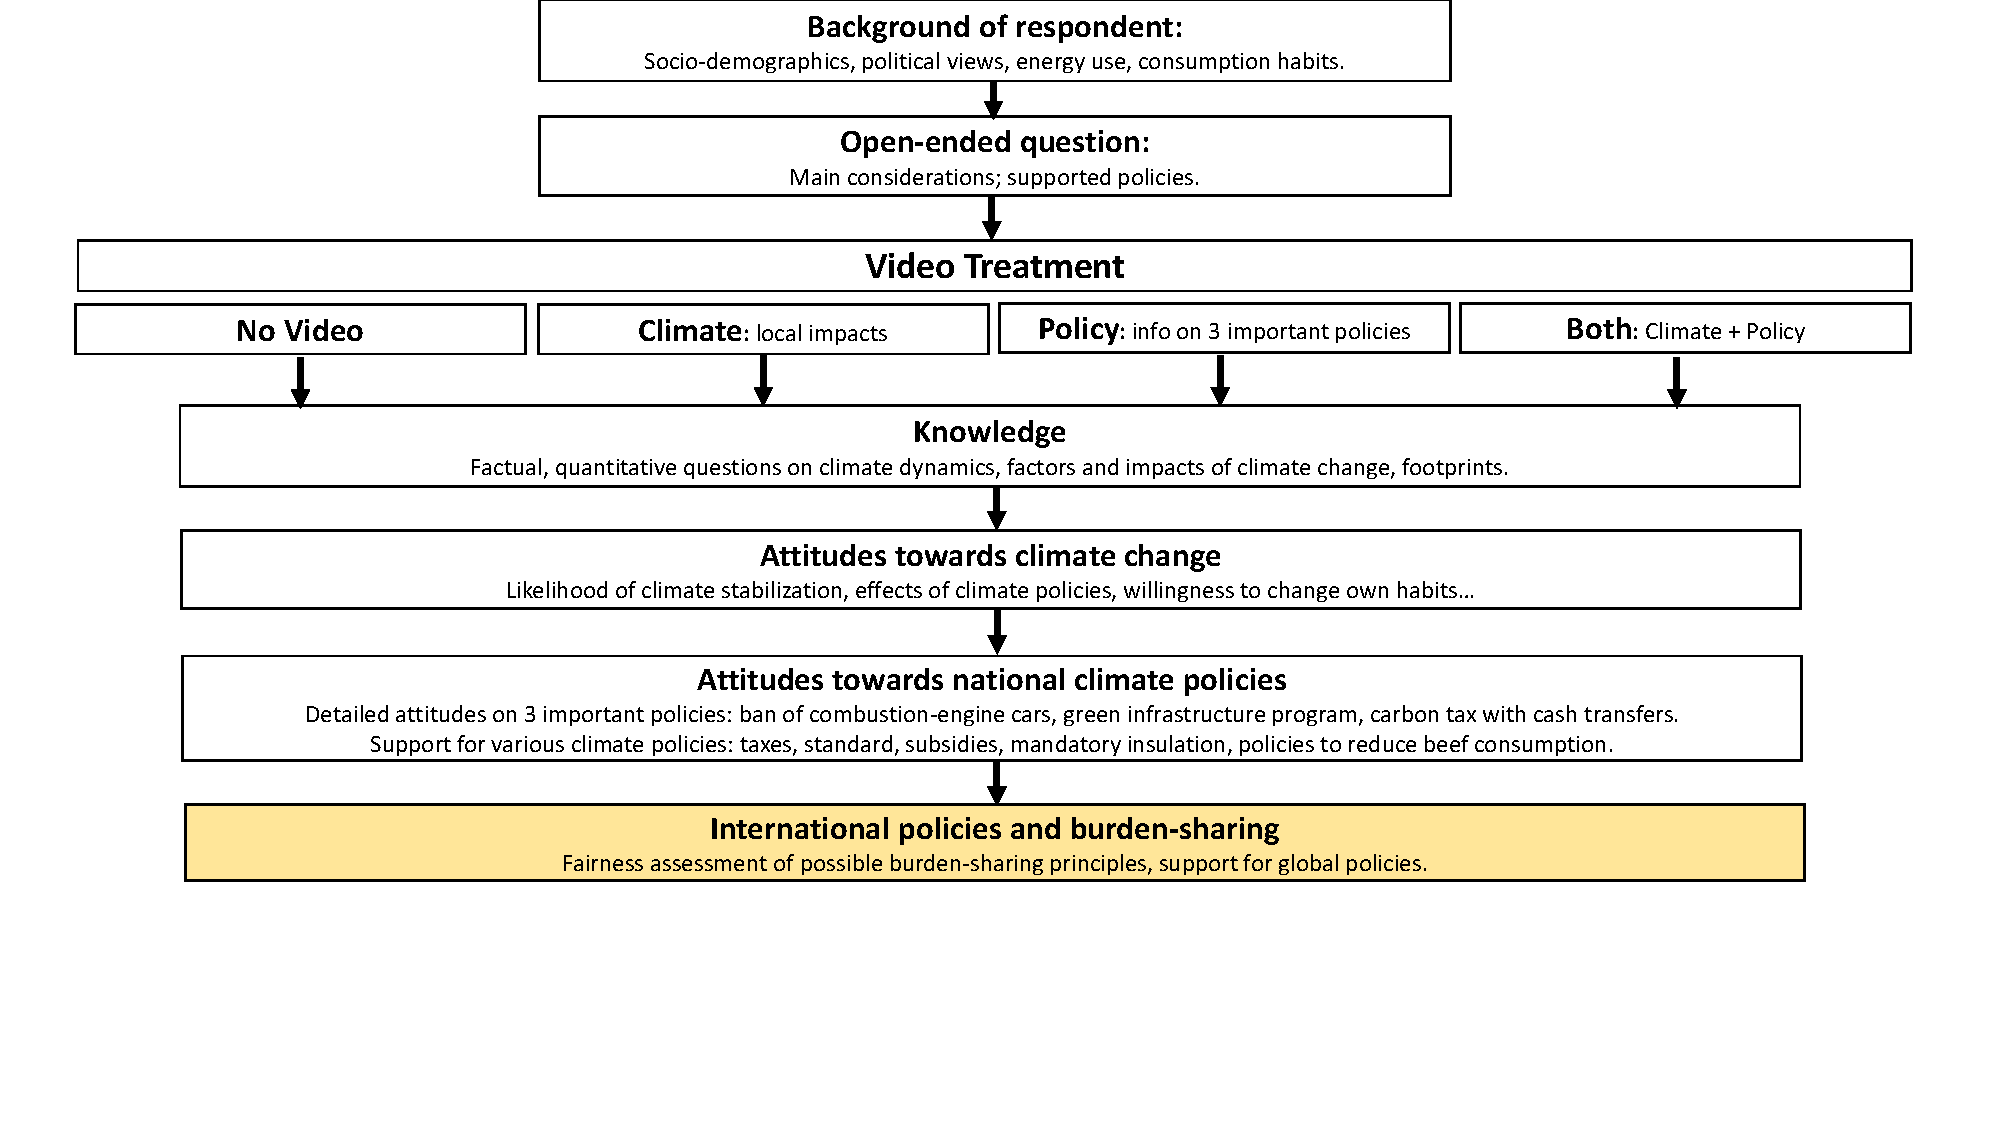
\includegraphics[width=.9\textwidth]{../figures/survey_flow/survey_flow_new-8.pdf}}}
\only<+>{\makebox[\textwidth][c]{ 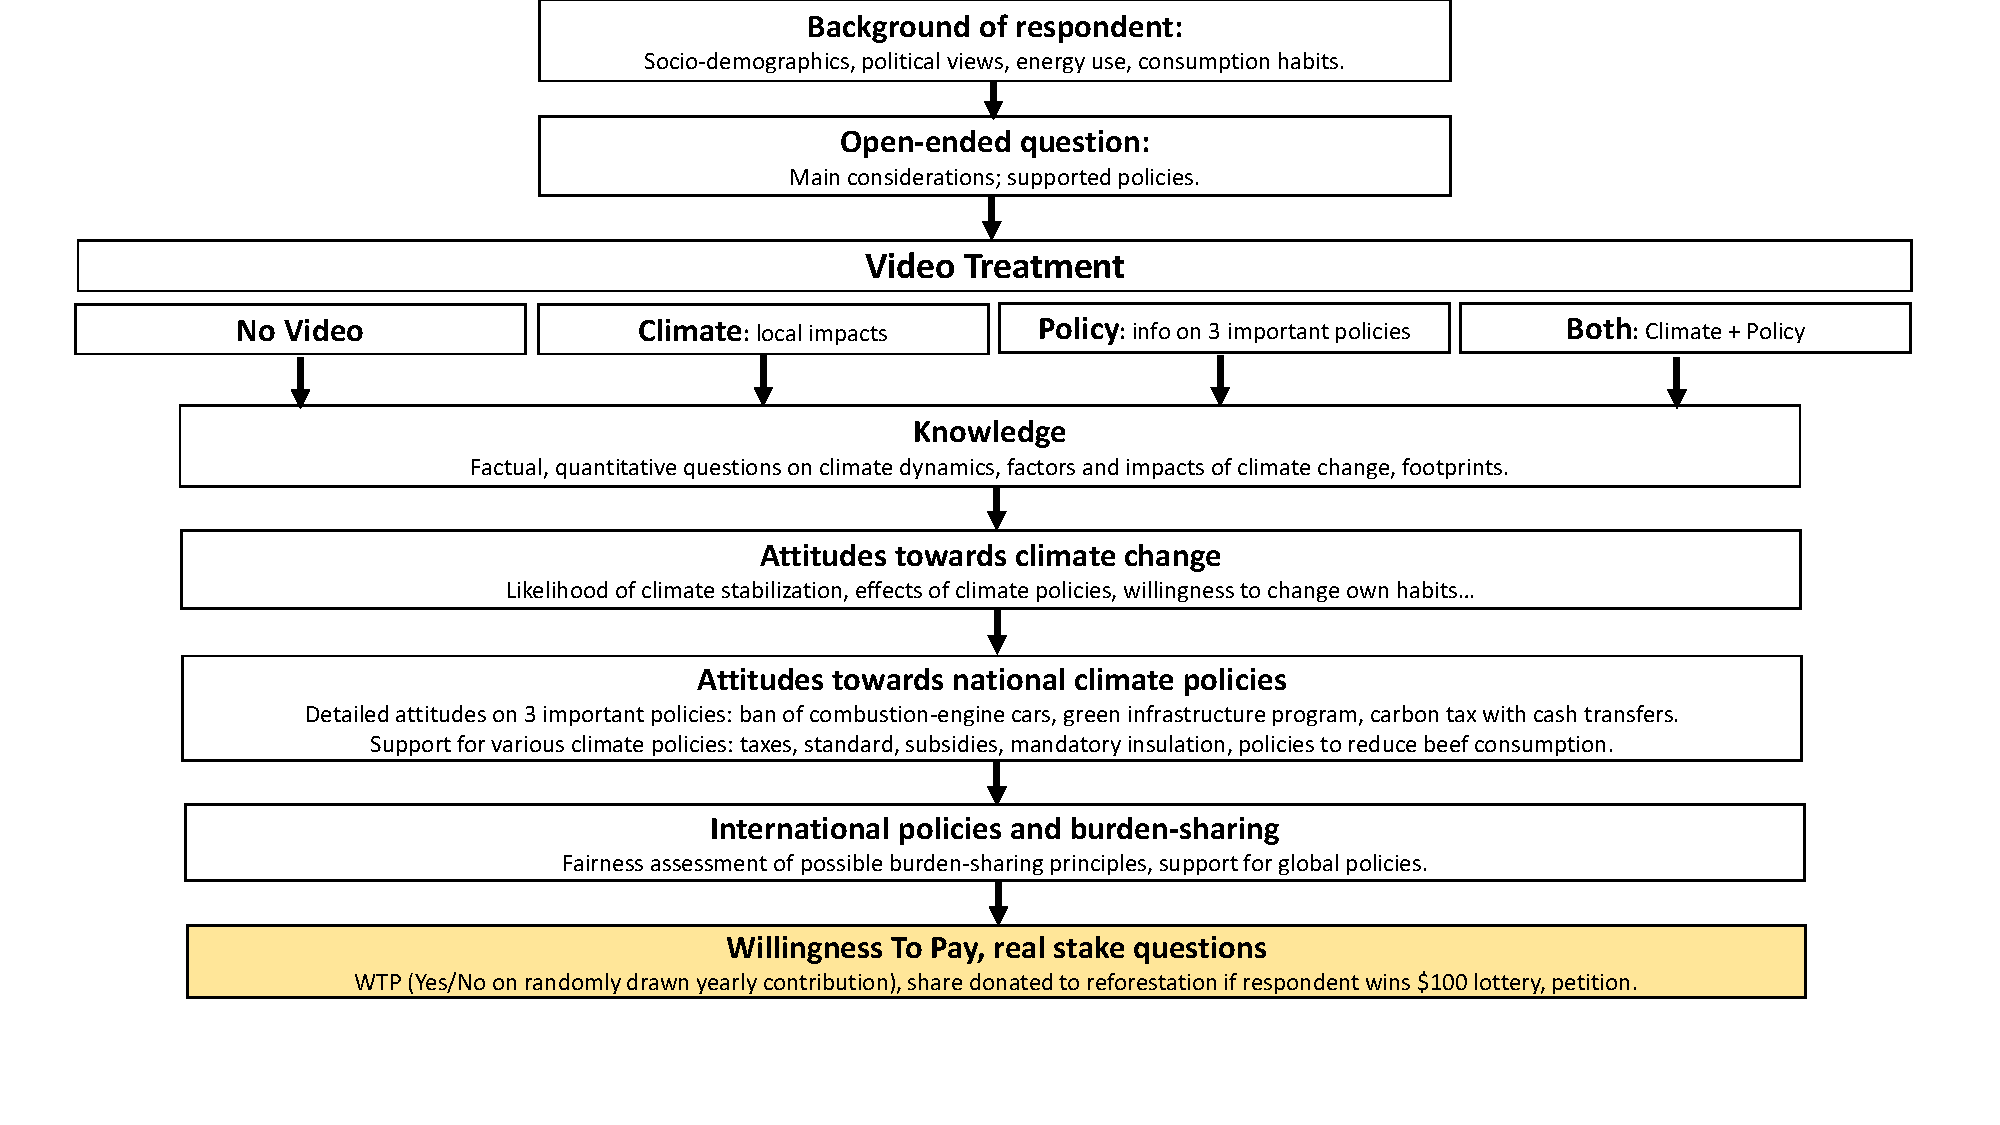
\includegraphics[width=.9\textwidth]{../figures/survey_flow/survey_flow_new-9.pdf}}}
\only<+>{\makebox[\textwidth][c]{ 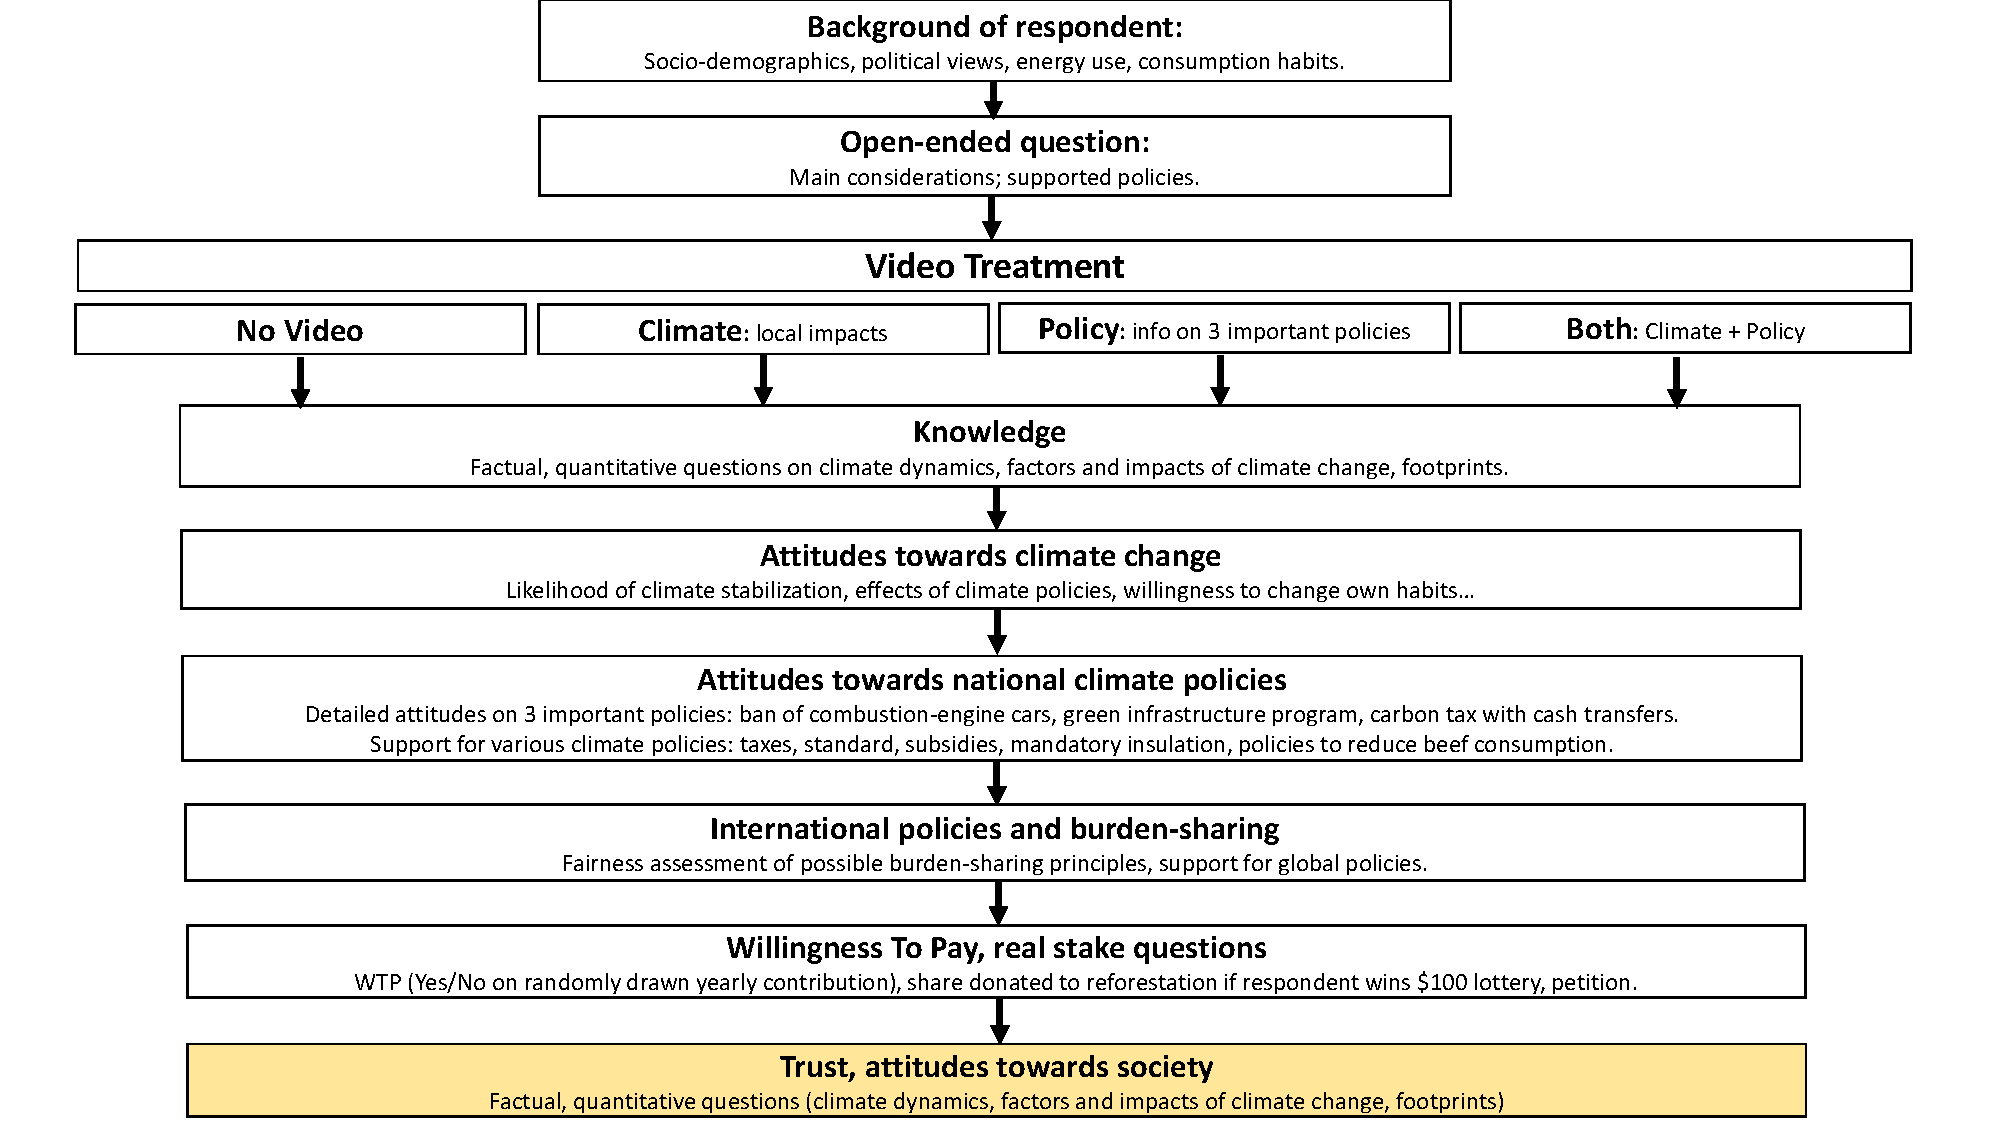
\includegraphics[width=.9\textwidth]{../figures/survey_flow/survey_flow_new-10.pdf}}}
\only<+>{\makebox[\textwidth][c]{ 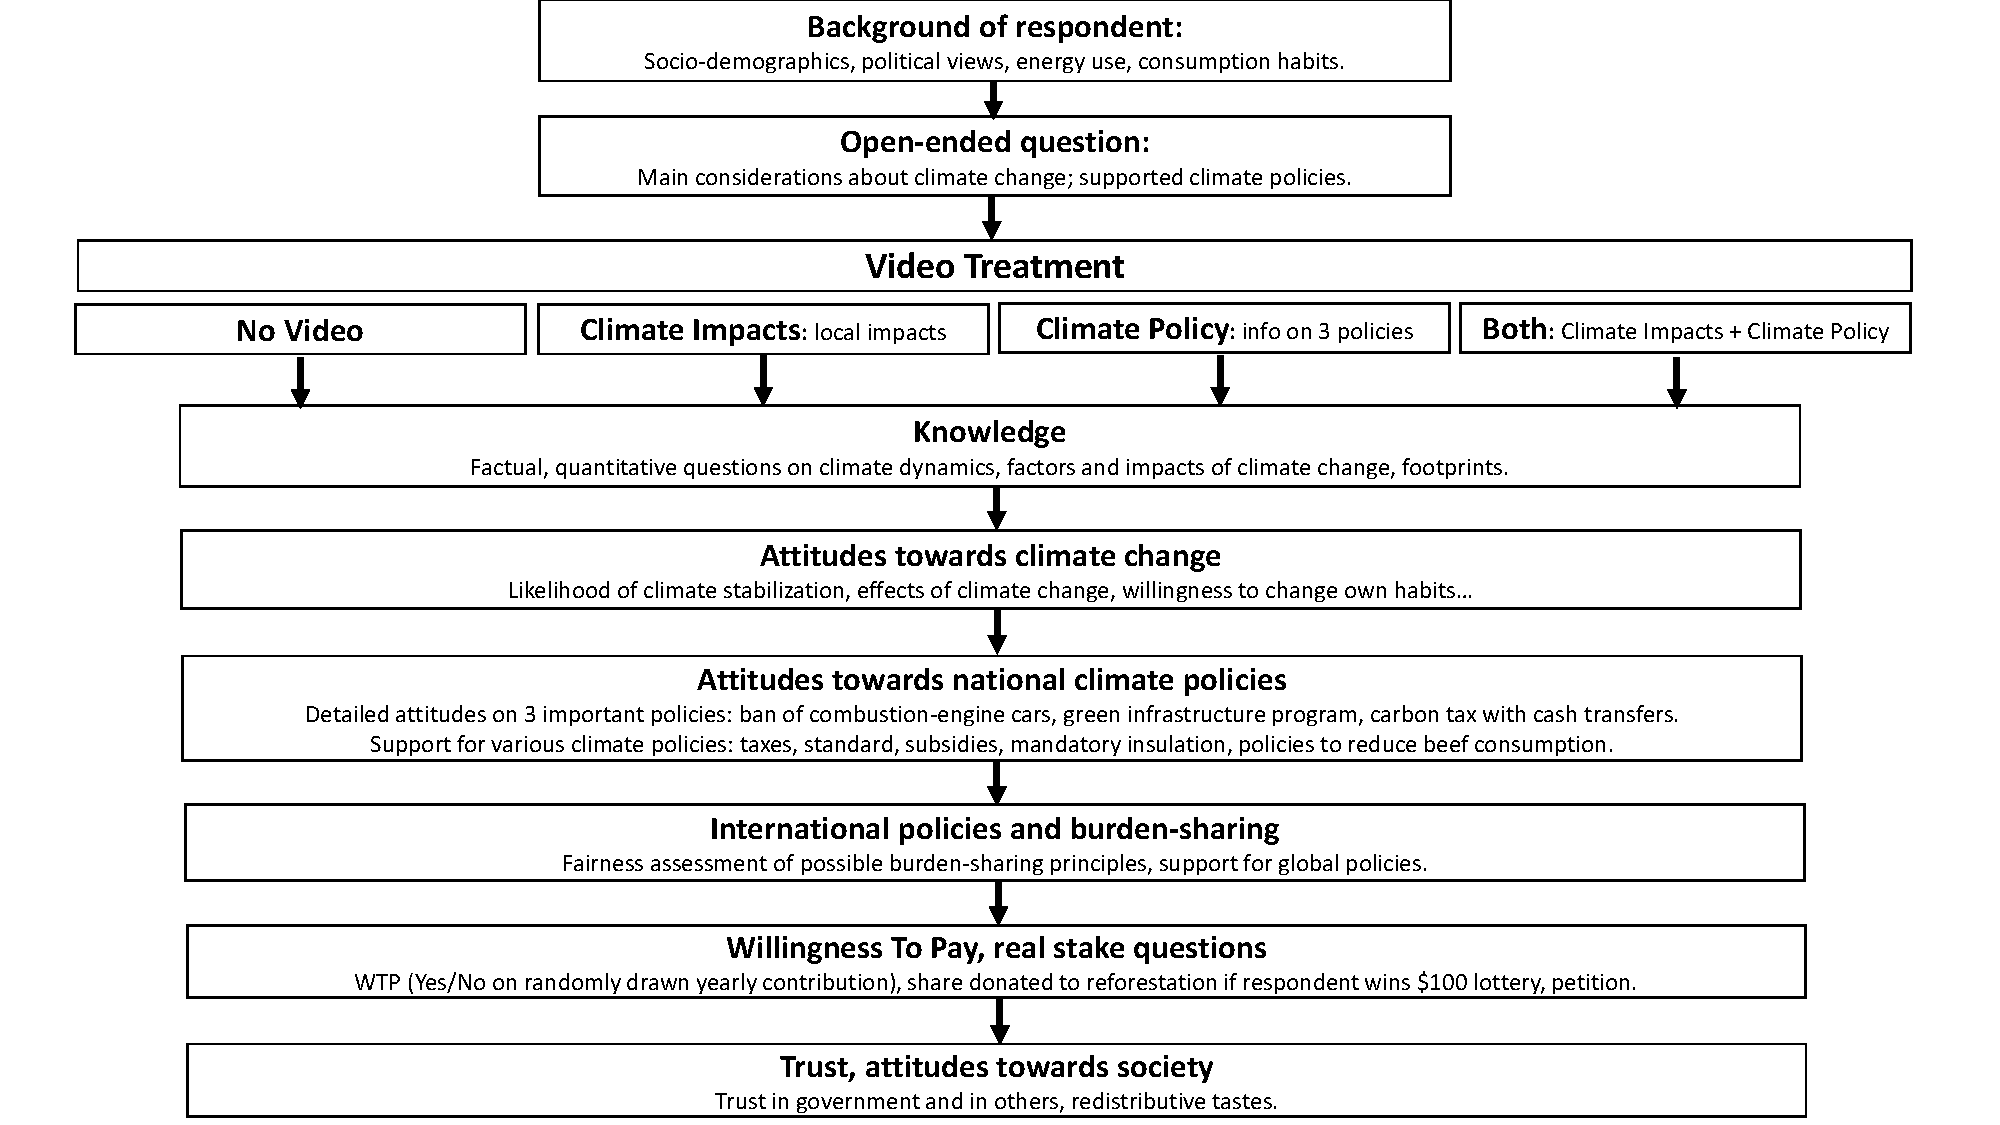
\includegraphics[width=.9\textwidth]{../figures/survey_flow/survey_flow_new-11.pdf}}}
%\end{itemize}
%}
\end{frame}

\section{Sample quality -- France}

%- Add more tables? Effect of misperception + heterogeneity (indices) for instance
%- Do we add something on the LDA ?%

%- In table underline some key lines ? Like in slide 36 here: https://scholar.harvard.edu/files/stantcheva/files/understanding_taxes_slides.pdf
%- Pour le moment la présentation est vraiment descriptive (liste les réponses à chaque question), mais est-ce que l'on veut faire ça ou avoir un narrative (à travers une research question à laquelle on veut réponse et en faisant des sections sur les résultats préliminaires que l'on a, plutôt que de grouper block par block - même si ça va sûrement être très proche)

\begin{frame}{Ensuring data quality}
\bbs
\ip 2,006 respondents selected through quotas that  \textcolor{blue}{ensure representativeness} along: \\ \textcolor{magenta}{gender, age, income, region, diploma, urban/rural}.
\ip \textcolor{blue}{All results are re-weighted} along quota variables (except rural/urban) to increase representativeness even further.
\ip \textcolor{blue}{Screening question} in the middle of the survey. 
\ip Appeal to people's social responsibility. 
\ip Warn that ``incoherent and \textcolor{blue}{rushed responses'' (< 11 min) are dismissed} and disqualified for monetary compensation.
\ip Record time spent on separate questions \& overall survey (median: 27 min).
\ip Ask for feedback post survey, whether felt survey was biased (\textcolor{magenta}{78\% find it unbiased}).
%\ip Check careless response patterns (clicking same ``middle'' answer).
\ee
\end{frame}

\begin{frame}{Representativeness of the Survey Sample}
\begin{table}[h!]
	%\caption{Sample Characteristics -- France}
	\begin{center}
		\scalebox{0.55}{\input{"../tables/FR/summary_stat_fr_prez"}}
	\end{center}
\end{table}	
\end{frame}

\begin{framefont}{\small}


\section{Knowledge}

\begin{frame}{Climate change acknowledged as serious problem but overlooked}%\addtocounter{framenumber}{-1}
	\begin{figure}[h!]
	\centering
	\caption{Do you agree or disagree with the following statement: ``Climate change is an important problem."}
	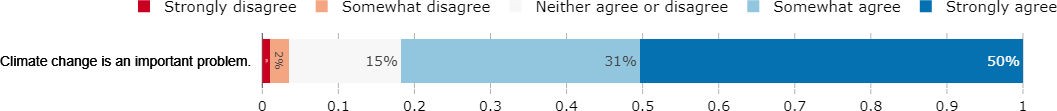
\includegraphics[width=.78\paperwidth]{../figures/FR/CC_problem_FR.png}
	\caption{How often do you think or talk with people about climate change?}
	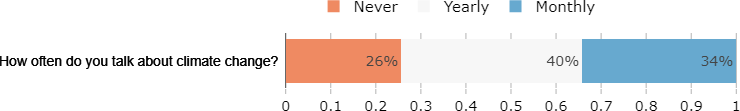
\includegraphics[width=.61\paperwidth]{../figures/FR/CC_talks_FR.png}\\
	\centering
	% \caption{In your opinion, is climate change real?} \\
	% 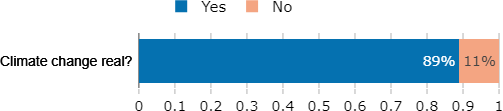
\includegraphics[width=.43\paperwidth]{../figures/FR/CC_real_FR.png} \\
	% \centering
	% \caption{\textit{If answered yes to previous question:} What part of climate change do you think is due to human activity?}
	% 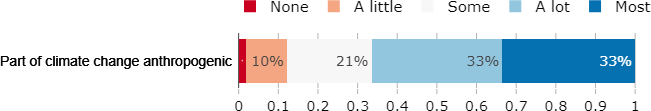
\includegraphics[width=.52\paperwidth]{../figures/FR/CC_anthropogenic_non_deniers_FR.png} # TOOD choose
	\caption{How knowledgeable do you consider yourself about climate change?}
	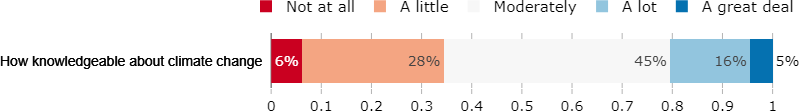
\includegraphics[width=.7\paperwidth]{../figures/FR/CC_knowledgeable_FR.png}
	\\
	\end{figure}
\end{frame}

\subsection{What are people relatively well aware of?}
% \begin{frame}{What are people relatively well aware of?} % Key Knowledge	
% \end{frame}

\begin{frame}{Impacts of climate change: Credit a lot of effects}%\addtocounter{framenumber}{-1}
\begin{figure}[h!]
\centering
%\caption{Impacts of climate change}
%\vspace{2mm}
\caption{If nothing is done to limit climate change, how likely do you think it is that climate change will lead to the following events?
\newline\footnotesize{\textit{Right answer: Very likely: Severe droughts and heatwaves; Rising sea levels \\ \quad \quad \quad \quad \quad \quad Very unlikely: More frequent volcanic eruptions (No scientific certainty on the other items)}}}
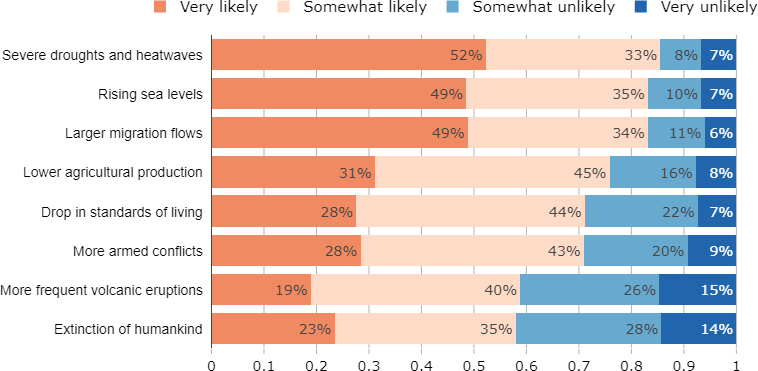
\includegraphics[width=.74\paperwidth]{../figures/FR/CC_impacts_FR.png} \\
%\caption{}
\end{figure}
\end{frame}

\begin{frame}{Not so many mistakes on the factors of climate change}%\addtocounter{framenumber}{-1}
	\begin{figure}[h!]
	\centering
	\caption{Which of the following elements contribute to climate change? (Multiple answers are possible) \newline \footnotesize{\textit{Right answer: CO$_\text{2}$; Methane}}}
	\centering
	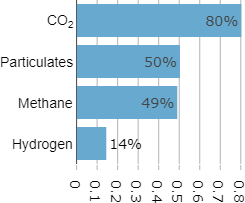
\includegraphics[width=.30\paperwidth]{../figures/FR/GHG_FR.png}
	\vspace{.2cm} \\
	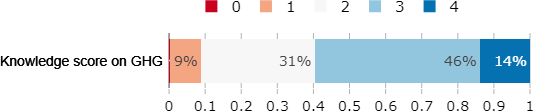
\includegraphics[width=.61\paperwidth]{../figures/FR/score_GHG_FR.png}
	
	\textit{Score on GHG = CO$_\text{2}$ + methane + }not\textit{ hydrogen + }not\textit{ particulates}
	%\caption{Which of the following elements contribute to climate change? (Multiple answers are possible))}
	\end{figure}
\end{frame}
	
	
\begin{frame}{}%Climate change knowledge: Know relative emissions}
	\begin{columns}
	\begin{column}{0.5\textwidth}
	\begin{figure}
	\caption{Which dish emits the most greenhouse gases? We consider that each dish weighs 200g.
	Please rank the items from 1 (most) to 3 (least).
	\newline \footnotesize{\textit{Right answer: Beef (1), Chicken (2), Pasta (3)}}}
	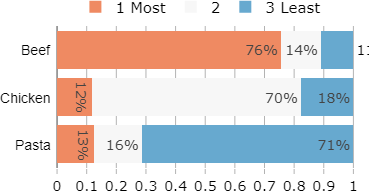
\includegraphics[width=.43\paperwidth]{../figures/FR/footprint_food_FR.png}
	\end{figure}
	\end{column}
	\begin{column}{0.5\textwidth}
	\begin{figure}
	\caption{If a family of 4 travels 800 km from Bordeaux to Nice, with which mode of transportation do they emit the most greenhouse gases? 
	Please rank the items from 1 (most) to 3 (least).
	\newline \footnotesize{\textit{Right answer: Plane (1), Car (2), Train (3)}}} % TODO:other_countries Coach, towns
	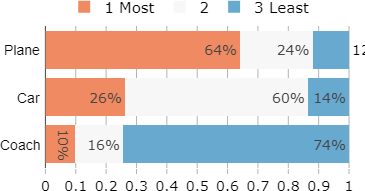
\includegraphics[width=.43\paperwidth]{../figures/FR/footprint_transport_FR.png}
	\end{figure}
	\end{column}
	\end{columns}
\end{frame}
	
\begin{frame}{}%Climate change knowledge: Understand role of coal but misinformed about nuclear}%\addtocounter{framenumber}{-1}
	\begin{figure}
	\caption{Which source of electric energy emits the most greenhouse gases to provide power for a house?
	\newline \footnotesize{\textit{Right answer: Coal (1), Gas (2), Nuclear (3)}}}
	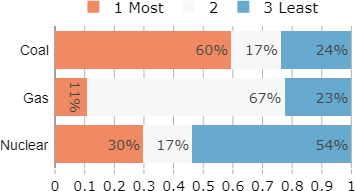
\includegraphics[width=.43\paperwidth]{../figures/FR/footprint_elec_FR.png}
	\end{figure}
\end{frame}
	
\subsection{What do people misperceive?}
\begin{frame}{Underestimation of EU emissions}%\addtocounter{framenumber}{-1}
	\begin{figure}[h!]
	\centering
	\begin{subfigure}[b]{0.425\paperwidth}
	\centering
	\caption{Which region contributes most to global greenhouse gas emissions?
	\newline \footnotesize{\textit{Right answer: China (1), US (2), EU (3), India (4)}}} % True ranking: China>US>EU>India. 
	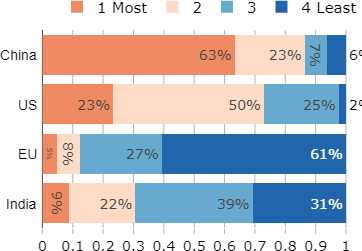
\includegraphics[width=.425\paperwidth]{../figures/FR/footprint_region_no_miss_FR.png}
	\end{subfigure}
	\hfill
	\begin{subfigure}[b]{0.425\paperwidth}
	\centering
	\caption{In which region does the consumption of an average person contribute most to climate change?
	\newline \footnotesize{\textit{Right answer: US (1), EU (2), China (3), India (4)}}} % True ranking: US>EU>China>India. 
	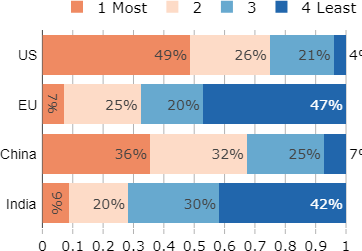
\includegraphics[width=.425\paperwidth]{../figures/FR/footprint_pc_no_miss_FR.png}
	\end{subfigure}
	\end{figure}
\end{frame}

\begin{frame}{Limited understanding of climate science}%\addtocounter{framenumber}{-1}
	\begin{figure}%[h!]
	\centering
	\caption{What part of climate change do you think is due to human activity? \footnotesize{\textit{Right answer: Most}}}
	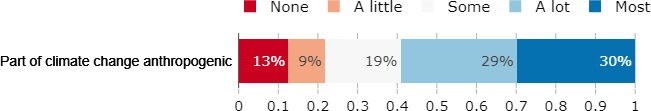
\includegraphics[width=.7\paperwidth]{../figures/FR/CC_anthropogenic_FR.png} 
	\\
	%\centering
	%\centering
	\caption{Do you think that cutting global greenhouse gas emissions by half would be sufficient to eventually stop temperatures from rising? \footnotesize{\textit{Right answer: No}}}
	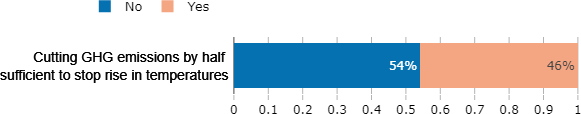
\includegraphics[width=.6\paperwidth]{../figures/FR/CC_dynamic_FR.png}
	
	\end{figure}
\end{frame}
% \begin{frame}{What do people misperceive?} % Key Misperceptions
	
% \end{frame}

\begin{frame}{Incidence: Carbon tax with cash transfers}%\addtocounter{framenumber}{-1}
	\begin{figure}[h!]
	\centering
	\caption{In your view, would the following groups win or lose under a carbon tax with cash transfers?}
	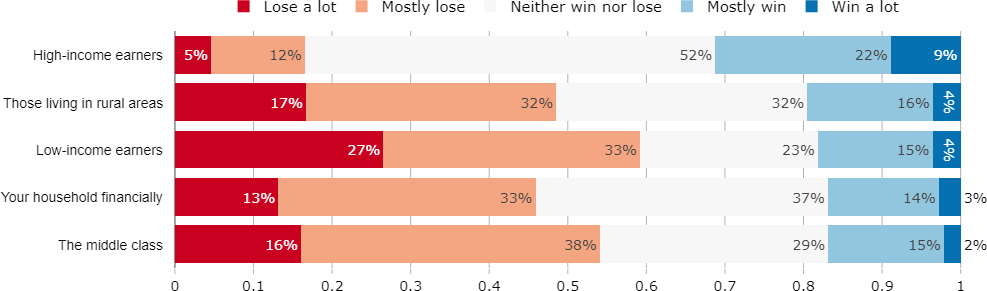
\includegraphics[width=.87\paperwidth]{../figures/FR/tax_transfers_win_lose_FR.png}
	%\caption{}
	\end{figure}
\end{frame}

\begin{frame}{Incidence: Green infrastructure program}%\addtocounter{framenumber}{-1}
	\begin{figure}[h!]
	\centering
	\caption{In your view, would the following groups win or lose with a green infrastructure program?}
	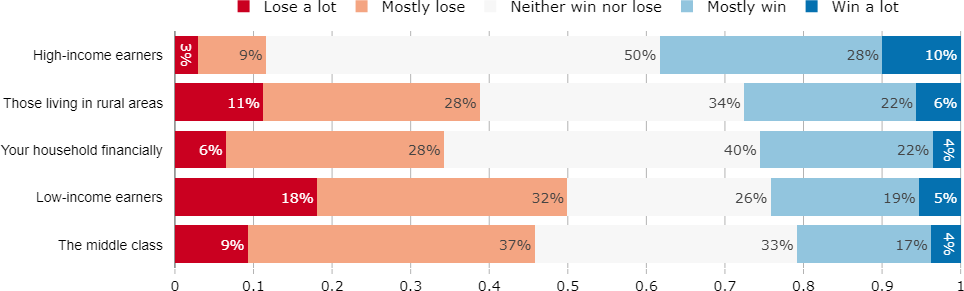
\includegraphics[width=.87\paperwidth]{../figures/FR/investments_win_lose_FR.png}
	%\caption{}
	\end{figure}
\end{frame}
	
	% \begin{frame}{Incidence: Ban on combustion-engine cars}%\addtocounter{framenumber}{-1}
% 	\begin{figure}[h!]
% 	\centering % TODO! harmonize order
% 	\caption{In your view, would the following groups win or lose if a ban on combustion-engine cars was implemented in France?}
% 	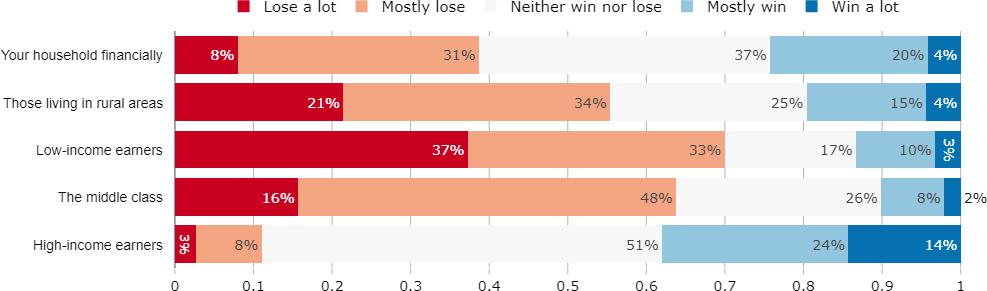
\includegraphics[width=.87\paperwidth]{../figures/FR/standard_win_lose_FR.png}
% 	%\caption{}
% 	\end{figure}
% \end{frame}

\begin{frame}{Who has better knowledge?}
	% One section on “Who has better knowledge?” Just a regression of some summary measure of knowledge on individual characteristics. 
% TODO! CC_anthropogenic / index_knowledge ~ setA (+B)
% Policy message of this section 
% Who knows more? Where is key info lacking (that policy makers should fix).  
\end{frame}

\section{Who supports what?}% Who supportes climate policies % Support for climate policies

\begin{frame}{France is in the OECD average, global policies strongly supported}
	\begin{figure}[h!]
		\centering		
		\caption{Share of support (somewhat or strongly) to the main policies.}
		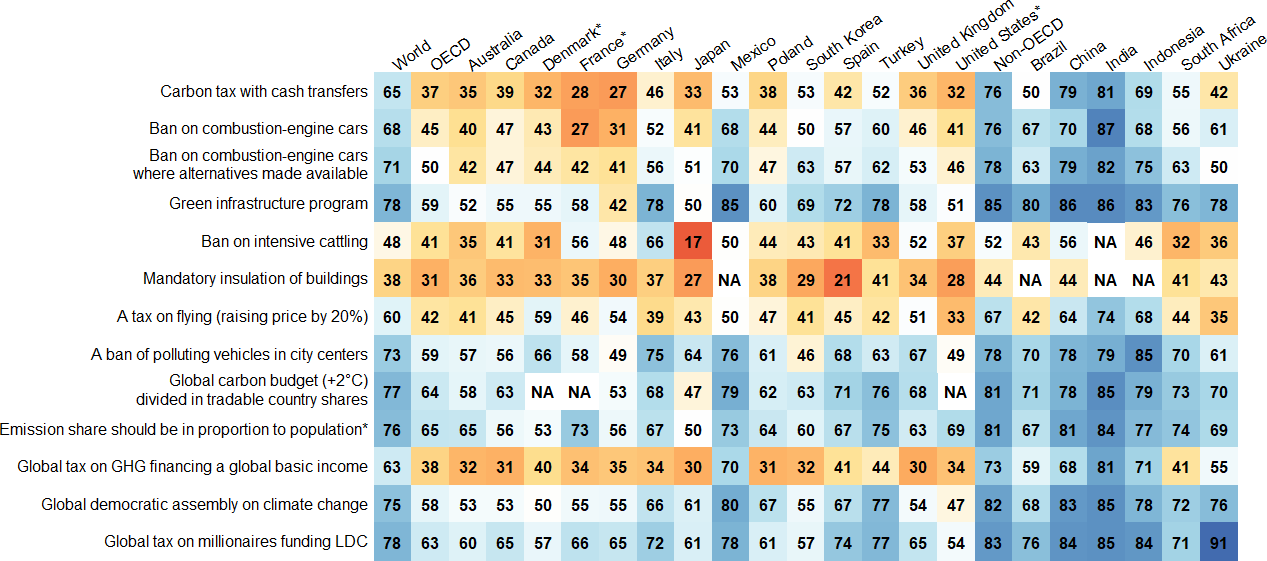
\includegraphics[width=\textwidth]{../figures/country_comparison/main_policies_positive_countries.png}
		%\caption{}
		\end{figure}
\end{frame}

\begin{frame}{France is in the OECD average, global policies strongly supported}
	\begin{figure}[h!]
		\centering		
		\caption{Share of support to the main policies among non-Indifferent.}
		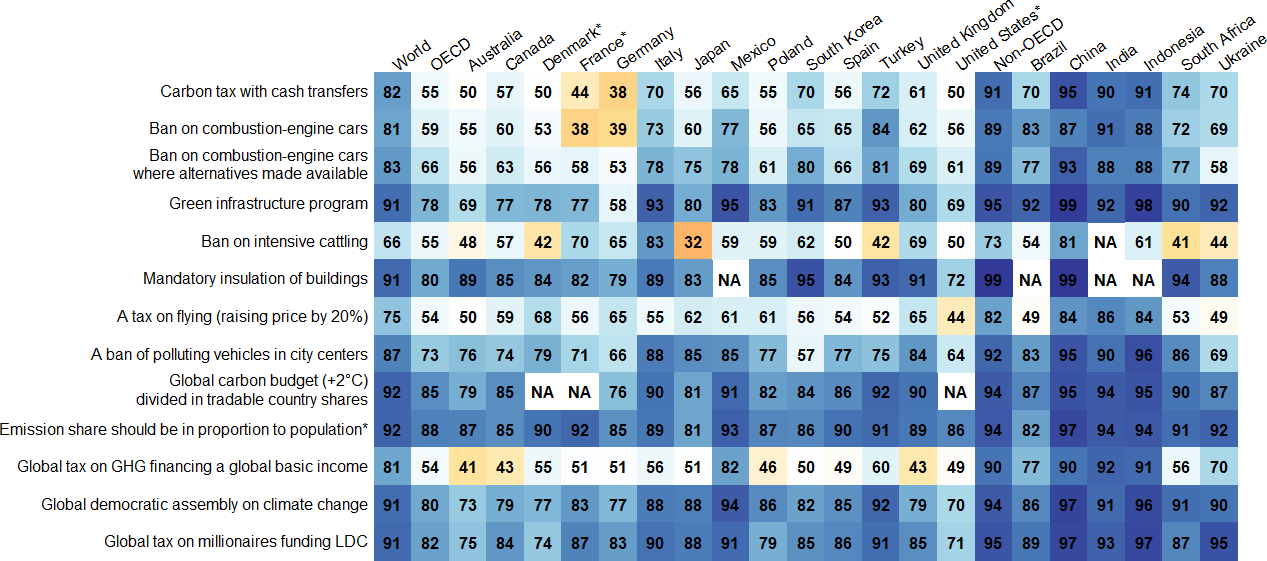
\includegraphics[width=\textwidth]{../figures/country_comparison/main_policies_share_countries.png}
		%\caption{}
		\end{figure}
\end{frame}

\begin{frame}{How support varies by socio-demographics}
	% Regress Outcomes on set A and set B. Identify main patterns. 
% In Appendix: Full regression tables. 
% In paper: 4-5 of they key heterogeneities, shown in graphical format. For instance, Tobias already identified that driving and relying on energy was important; Adrien pointed to age. 
% TODO!	 support_policies/index_policies ~ setA + B; plot_along (with only one outcome on the y axis) by children, age, diploma, urban/rural, availability transport, YV, vote, gas expenses
\end{frame}

\begin{frame}{Zooming on regression results}
\begin{figure}[h!]	
	\caption{Effects of living with child(ren) < 14, age, and having a college degree, on support for main policies, conditional on socio-demographics (set A) and energy characteristics (B).}
	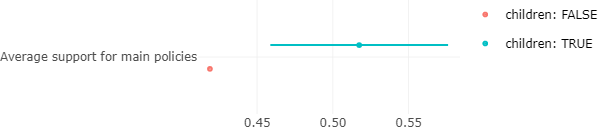
\includegraphics[width=.7\textwidth]{../figures/FR/policies_support_by_children.png}
	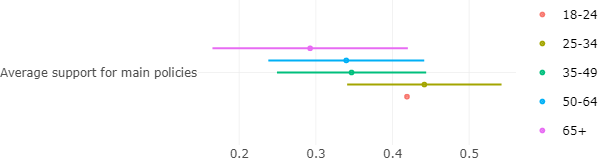
\includegraphics[width=.7\textwidth]{../figures/FR/policies_support_by_age.png}
	
\includegraphics[width=.7\textwidth]{../figures/FR/policies_support_by_college.png}
\end{figure}
\end{frame}

\begin{frame}{Zooming on regression results}
\begin{figure}[h!]	
	\caption{Effects of living in an urban ``Grand Pôle'' and position on the Yellow Vests, on support for main policies, conditional on socio-demographics (set A) and energy characteristics (B).}
	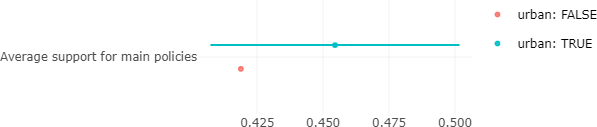
\includegraphics[width=.7\textwidth]{../figures/FR/policies_support_by_urban.png}
	\vspace{0.8cm}
	\caption{Yellow Vests positioning:}
	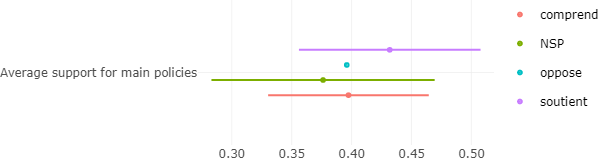
\includegraphics[width=.7\textwidth]{../figures/FR/policies_support_by_Gilets_jaunes_agg.png}
	%\includegraphics[width=.7\textwidth]{../figures/FR/vote_agg.png}
\end{figure}
\end{frame}

% \begin{frame}{Zooming on regression results}
% \begin{figure}[h!]	
% 	\caption{Effects of the availability of public transport and gas expenses, on support for main policies, conditional on socio-demographics (set A) and energy characteristics (B).}
% 	\includegraphics[width=.7\textwidth]{../figures/FR/availability_transport.png}
% 	\includegraphics[width=.7\textwidth]{../figures/FR/gas_expenses.png}
% 	%\includegraphics[width=.7\textwidth]{../figures/FR/vote_agg.png}
% \end{figure}
% \end{frame}

\begin{frame}{What are the different \textit{types} of people?}
	% LDA analysis to identify “types” of respondents. 
% TODO! 
\end{frame}


\section{What ideas can explain support for climate policies?}

\begin{frame}{Main mechanisms}
	% A. Mechanisms. 
% Regress Outcomes on set C + set A (—> answers the question of what type of thinking needs to changed 
% (We already did nice figures like this, but we needed to reorganize what was a mechanism and what was an outcome) 
% TODO! support_policies/index_policies ~ setA + B + C; variance decomposition support_policies/index_policies
\end{frame}

\begin{frame}{The distributional dimension}
\begin{figure}
	\vspace{-.2cm}
	\caption{%Until now, we have considered that a green infrastructure program would be financed by public debt, but other sources of funding are possible.\\
	What sources of funding do you find appropriate for public investments in green infrastructure? (Multiple answers are possible)}
	\vspace{-.4cm}
	\includegraphics[width=.45\paperwidth]{../figures/FR/investments_funding_FR.png}
	\caption{How important are the factors below in order for you to adopt a sustainable lifestyle (i.e. limit driving, flying, and consumption, cycle more, etc.)?}
	\vspace{-.4cm}
	\includegraphics[width=.7\paperwidth]{../figures/FR/condition_FR.png}
\end{figure}
	% TODO!: variance_decomp with fairness in the regressors, desc stats on investments_funding, condition(_rich_change)...
\end{frame}

\begin{frame}{What ideas explain differentiated support among social groups?}
	% B. Gelbach decompositions of the key heterogeneities (e.g.: what makes people of different ages support different policies) into the mechanisms of set C. 
	% TODO! Gelbach vote (also age, diploma)
\end{frame}

\begin{frame}{Can information change attitudes?}
	% C. Provide description of Treatments with screen shots. 
% Regress Outcomes on treatment indicators + set A. 
\begin{figure}
	\caption{Treatment effects in regressions of support indices on the set (A) of socio-demographics.}
	\includegraphics[width=.7\textwidth]{../figures/FR/policies_support_by_treatment.png}
	%\caption{How important are the factors below in order for you to adopt a sustainable lifestyle (i.e. limit driving, flying, and consumption, cycle more, etc.)?}
	\includegraphics[width=.7\textwidth]{../figures/FR/indices_policies_by_treatment_origin0.png}
\end{figure}
\end{frame}

\section{Conclusion}

\begin{frame}{Key take-home messages for policy-making}
\bbvs
\ip Widespread concern for climate change and large support for global climate policies.
\ip Majority support for a green infrastructure program
\ip Mixed support for a carbon tax with cash transfers and a ban of combustion-engine cars. % people want it to be clear that the rich pay for the provision of new infrastructure rather than having to pay for themselves and compensated ex post 
%\ip Majority support for different norms and regulations.
\ip Attitudes are largely idiosyncratic.
\ip Availability of decarbonized alternatives like public transport is key. 
\ip The distributional fairness of the policy packge is critical for the acceptance of many people. \\ $\Rightarrow$ Make sure the policy package is progressive, and that people understand that.
%\ip Knowledge that climate change is anthropogenic and trust in government are key beliefs to support climate policies.
\ip Information can improve understanding of a carbon tax with cash transfers, and thereby increase support.
\ee
\end{frame}

\appendix
\section{Appendix}

\section{Descriptive statistics \\ \quad \\ on the control group}



% \begin{frame}{Hit by COVID-19}%\addtocounter{framenumber}{-1}
% \begin{figure}[h!]
% \centering
% \captionsetup{justification=centering}
% \caption{Have you or a member of your household been laid off or had to take a cut in your salary or wages due to the COVID-19 pandemic?}
% \includegraphics[width=.52\paperwidth]{../figures/FR/hit_by_covid_FR.png} # TODO choose
% \end{figure}
% \end{frame}

\subsection{Households characteristics}

\begin{frame}{Little interest for politics}%\addtocounter{framenumber}{-1}
\vspace{-.5cm}
\begin{figure}[h!]
\caption{To what extent are you interested in politics?}
\includegraphics[width=.52\paperwidth]{../figures/FR/interested_politics_FR.png} \\
%\caption{Could you trust the federal goverment to implement the following policies}
\vspace{.1cm}
\caption{Are you member of an environmental organization?}
\includegraphics[width=.47\paperwidth]{../figures/FR/member_environmental_orga_FR.png}\\
\vspace{.1cm}
\caption{Do you have any relatives who are environmentalists?}
\includegraphics[width=.47\paperwidth]{../figures/FR/relative_environmentalist_FR.png}\\
\end{figure}
\end{frame}

\begin{frame}{Broadly representative political leaning}%\addtocounter{framenumber}{-1}
\vspace{-.5cm}
\begin{figure}[h!]
\caption{Did you vote in the 2017 French presidential election?}
\includegraphics[width=.45\paperwidth]{../figures/FR/vote_participation_FR.png} \\
%\caption{Could you trust the federal goverment to implement the following policies}
\vspace{.1cm}
\caption{Which candidate did you vote / would you have voted for in the last presidential election?}
\includegraphics[width=.7\paperwidth]{../figures/FR/vote_main_FR.png} \\
\caption{On economic policy matters, where do you see yourself on the left/right spectrum?}
\includegraphics[width=.7\paperwidth]{../figures/FR/left_right_FR.png}
% \caption{Which candidate did you vote for in the last presidential election?}
% \includegraphics[width=.52\paperwidth]{../figures/FR/vote_all_FR.png} \\
% \caption{Did you vote in the 2016 French presidential election?}
% \includegraphics[width=.47\paperwidth]{../figures/FR/vote_participation_2016_FR.png}\\
\end{figure}
\end{frame}

%\begin{frame}{Uniform Political affiliation}%\addtocounter{framenumber}{-1}
%\vspace{-.5cm}
%\begin{figure}[h!]
%\caption{On economic policy matters, where do you see yourself on the left/right spectrum?}
%\includegraphics[width=.7\paperwidth]{../figures/FR/left_right_FR.png} \\
%%\caption{Could you trust the federal goverment to implement the following policies}
%%\vspace{.1cm}
%%\caption{What do you consider to be your political affiliation, as of today?}
%%\includegraphics[width=.7\paperwidth]{../figures/FR/political_affiliation_FR.png}\\
%\end{figure}
%\end{frame}


\begin{frame}{Drivers more than fliers}%\addtocounter{framenumber}{-1}
\begin{figure}[h!]
\centering
\caption{Which mode of transport did you mainly use for each of the following trips in 2019?}
\includegraphics[width=.61\paperwidth]{../figures/FR/transport_FR.png} \\
\vspace{.5cm}
\caption{How many round-trip flights did you take between 2017 and 2019?}
\includegraphics[width=.61\paperwidth]{../figures/FR/flights_3y_FR.png}
%\caption{How do you rate the availability (ease of access and frequency) of public transportation where you live?}
%\includegraphics[width=.78\paperwidth]{../figures/FR/availability_transport_FR.png}
\end{figure}
\end{frame}



\subsection{Climate Knowledge}

%\begin{frame}{Climate knowledge: summary} % TODO
%    \begin{itemize}
%    \item People worry; knowledge is mixed.
%        \item In line with previous research, we find that about 60\% of Americans acknowledge that climate change exists and is anthropogenic.
%        \item A majority under-estimate the stringency of needed emission reductions. 
%        \item Most people understand what activities are most polluting, except for transport where knowledge is mixed. Most struggle identifying the correct ranking of regional per capita footprint.
%        \item Most people correctly understand that climate change will entail more natural disasters, but wrongly think that volcanic eruptions will be more frequent.
%        \item A majority thinks that CC puts humanity at risk of extinction, which is extremely pessimistic.
%        \item A relative majority thinks they will be personally affected by CC.
%    \end{itemize}
%\end{frame}

\begin{frame}{Climate change acknowledged as serious problem but overlooked}%\addtocounter{framenumber}{-1}
\begin{figure}[h!]
\centering
\caption{Do you agree or disagree with the following statement: ``Climate change is an important problem."}
\includegraphics[width=.78\paperwidth]{../figures/FR/CC_problem_FR.png}
\caption{How often do you think or talk with people about climate change?}
\includegraphics[width=.61\paperwidth]{../figures/FR/CC_talks_FR.png}\\
\centering
% \caption{In your opinion, is climate change real?} \\
% \includegraphics[width=.43\paperwidth]{../figures/FR/CC_real_FR.png} \\
% \centering
% \caption{\textit{If answered yes to previous question:} What part of climate change do you think is due to human activity?}
% \includegraphics[width=.52\paperwidth]{../figures/FR/CC_anthropogenic_non_deniers_FR.png} # TOOD choose
\caption{How knowledgeable do you consider yourself about climate change?}
\includegraphics[width=.7\paperwidth]{../figures/FR/CC_knowledgeable_FR.png}
\\
\end{figure}
\end{frame}

\begin{frame}{Limited understanding of climate science}%\addtocounter{framenumber}{-1}
\begin{figure}%[h!]
\centering
\caption{What part of climate change do you think is due to human activity? \footnotesize{\textit{Right answer: Most}}}
\includegraphics[width=.7\paperwidth]{../figures/FR/CC_anthropogenic_FR.png} 
\\
%\centering
%\centering
\caption{Do you think that cutting global greenhouse gas emissions by half would be sufficient to eventually stop temperatures from rising? \footnotesize{\textit{Right answer: No}}}
\includegraphics[width=.6\paperwidth]{../figures/FR/CC_dynamic_FR.png}

\end{figure}
\end{frame}

\begin{frame}{Some mistakes on the factors of climate change}%\addtocounter{framenumber}{-1}
\begin{figure}[h!]
\centering
\caption{Which of the following elements contribute to climate change? (Multiple answers are possible) \newline \footnotesize{\textit{Right answer: CO$_\text{2}$; Methane}}}
\centering
\includegraphics[width=.30\paperwidth]{../figures/FR/GHG_FR.png}
\vspace{.2cm} \\
\includegraphics[width=.61\paperwidth]{../figures/FR/score_GHG_FR.png}

\textit{Score on GHG = CO$_\text{2}$ + methane + }not\textit{ hydrogen + }not\textit{ particulates}
%\caption{Which of the following elements contribute to climate change? (Multiple answers are possible))}
\end{figure}
\end{frame}

% out
% \begin{frame}{Climate change knowledge: GHG footprints}%\addtocounter{framenumber}{-1}
% \begin{figure}[h!]
% \centering
% % \caption{Number of errors when ranking 3 items in terms of GHG emissions for three sectors}
% \caption{Kendall tau distance to correct ranking of GHG footprints for three sectors ($\sim$ number of mistakes)}
% \includegraphics[width=.43\paperwidth]{../figures/FR/scores_footprint_FR.png} \\
% \centering
% \caption{Rank the French/China/Western Europe/India in terms of GHG footprint}
% \includegraphics[width=.52\paperwidth]{../figures/FR/score_footprint_regions_FR.png}
% \vspace{.2cm}
% % \\
% % \small{Correct ranking: plane>car>coach, beef>chicken>pasta, coal>gas>wind/ US>Western Europe>China>India} \\
% \end{figure}
% \end{frame}

\begin{frame}{}%Climate change knowledge: Know relative emissions}
\begin{columns}
\begin{column}{0.5\textwidth}
\begin{figure}
\caption{Which dish emits the most greenhouse gases? We consider that each dish weighs 200g.
Please rank the items from 1 (most) to 3 (least).
\newline \footnotesize{\textit{Right answer: Beef (1), Chicken (2), Pasta (3)}}}
\includegraphics[width=.43\paperwidth]{../figures/FR/footprint_food_FR.png}
\end{figure}
\end{column}
\begin{column}{0.5\textwidth}
\begin{figure}
\caption{If a family of 4 travels 800 km from Bordeaux to Nice, with which mode of transportation do they emit the most greenhouse gases? 
Please rank the items from 1 (most) to 3 (least).
\newline \footnotesize{\textit{Right answer: Plane (1), Car (2), Train (3)}}} % TODO:other_countries Coach, towns
\includegraphics[width=.43\paperwidth]{../figures/FR/footprint_transport_FR.png}
\end{figure}
\end{column}
\end{columns}
\end{frame}

\begin{frame}{}%Climate change knowledge: Understand role of coal but misinformed about nuclear}%\addtocounter{framenumber}{-1}
\begin{figure}
\caption{Which source of electric energy emits the most greenhouse gases to provide power for a house?
\newline \footnotesize{\textit{Right answer: Coal (1), Gas (2), Nuclear (3)}}}
\includegraphics[width=.43\paperwidth]{../figures/FR/footprint_elec_FR.png}
\end{figure}
\end{frame}

\begin{frame}{Underestimation of EU emissions}%\addtocounter{framenumber}{-1}
\begin{figure}[h!]
\centering
\begin{subfigure}[b]{0.425\paperwidth}
\centering
\caption{Which region contributes most to global greenhouse gas emissions?
\newline \footnotesize{\textit{Right answer: China (1), US (2), EU (3), India (4)}}} % True ranking: China>US>EU>India. 
\includegraphics[width=.425\paperwidth]{../figures/FR/footprint_region_no_miss_FR.png}
\end{subfigure}
\hfill
\begin{subfigure}[b]{0.425\paperwidth}
\centering
\caption{In which region does the consumption of an average person contribute most to climate change?
\newline \footnotesize{\textit{Right answer: US (1), EU (2), China (3), India (4)}}} % True ranking: US>EU>China>India. 
\includegraphics[width=.425\paperwidth]{../figures/FR/footprint_pc_no_miss_FR.png}
\end{subfigure}
\end{figure}
\end{frame}

\begin{frame}{Impacts of climate change: Credit a lot of effects}%\addtocounter{framenumber}{-1}
\begin{figure}[h!]
\centering
%\caption{Impacts of climate change}
%\vspace{2mm}
\caption{If nothing is done to limit climate change, how likely do you think it is that climate change will lead to the following events?
\newline\footnotesize{\textit{Right answer: Very likely: Severe droughts and heatwaves; Rising sea levels \\ \quad \quad \quad \quad \quad \quad Very unlikely: More frequent volcanic eruptions (No scientific certainty on the other items)}}}
\includegraphics[width=.74\paperwidth]{../figures/FR/CC_impacts_FR.png} \\
%\caption{}
\end{figure}
\end{frame}
% CC_dynamic

\subsection{Climate Attitudes}

% out
\begin{frame}{In principle, high support for climate action}% TODO:other_countries "US" \addtocounter{framenumber}{-1}
\begin{figure}[h!]
\centering
\caption{Do you agree or disagree with the following statement: ``France should take measures to fight climate change."}
\includegraphics[width=.87\paperwidth]{../figures/FR/should_fight_CC_FR.png} \\
\vspace{1cm}
\caption{How should French climate policies depend on what other countries do?}
\includegraphics[width=.87\paperwidth]{../figures/FR/if_other_do_FR.png} \\
\end{figure}
\end{frame}


%\begin{frame}{Climate attitudes: summary} % TODO
%    \begin{itemize}
%    \item Most people agree CC is a problem and ambitious policies are needed.
%    \item People are divided between optimistic and pessimistic (regarding future standards of living, technical feasibility to stop CC, and likelihood it will happen).
%    \item People are divided between those who foresee positive effects of climate policies and a third who foresees negative effects.
%    \item A third of people is willing to forego some comfort, two-thirds are willing to change behavior as long as it doesn't affect their comfort and they have enough financial means.
%    %   \item Only a slight majority recognizes that each of us are highly responsible for climate change, while around 70\% perceive companies are highly responsible for climate change.
%    %     \item People are divided about whether climate change can be halted by the end of the century, but only 20\% think ambitious policies are not important to halt it.
%    %     \item Around 20\% also think that ambitious policies would have strong negative effects on their lifestyle and around 30\% think ambitious policies would have negative effects on the French economy. 
%    %     \item It can be linked to the fact that only a minority is willing to adopt the most restrictive behaviors. Different types of constraints seem to influence their decisions.
%    \end{itemize}
%\end{frame}

\begin{frame}{Companies held responsible}%\addtocounter{framenumber}{-1}
\begin{figure}[h!]
\centering
\caption{To what extent are the following groups responsible for climate change in France?}
\includegraphics[width=.7\paperwidth]{../figures/FR/CC_responsible_FR.png}
\end{figure}
\end{frame}


\begin{frame}{Balance between optimistic and pessimistic}%\addtocounter{framenumber}{-1}
\begin{figure}[h!]
\caption{To what extent do you think that it is technically feasible to stop greenhouse gas emissions while maintaining satisfactory standards of living in France?}
\includegraphics[width=.7\paperwidth]{../figures/FR/net_zero_feasible_FR.png} \\
\caption{To what extent do you think climate change already affects or will negatively affect your personal life?}
\includegraphics[width=.9\paperwidth]{../figures/FR/CC_affects_self_FR.png} \\
% \caption{How ambitious do you think public policies should be to halt climate change?}
% \includegraphics[width=.61\paperwidth]{../figures/FR/pro_ambitious_policies_FR.png}
\end{figure}
\end{frame}

\begin{frame}{}%Doubtful about ambitious climate policies effects}%\addtocounter{framenumber}{-1}
\begin{figure}[h!]
\centering
\caption{How likely is it that human kind halt climate change by the end of the century?}
\includegraphics[width=.61\paperwidth]{../figures/FR/CC_will_end_FR.png}\\
\caption{If we decide to halt climate change through ambitious policies, to what extent do you think it would negatively affect your lifestyle?}
\includegraphics[width=.61\paperwidth]{../figures/FR/effect_halt_CC_lifestyle_FR.png} \\
\caption{If we decide to halt climate change through ambitious policies, what would be the effects on the French economy and employment?} % TODO:other_countries "U.S "
\includegraphics[width=.61\paperwidth]{../figures/FR/effect_halt_CC_economy_FR.png}
\end{figure}
\end{frame}

\begin{frame}{Willing to adopt the less restrictive behaviors}%\addtocounter{framenumber}{-1}
\begin{figure}[h!]
\centering
\caption{Here are possible habits that experts say would help reduce greenhouse gas emissions.
To what extent would you be willing to adopt the following behaviors?}
\includegraphics[width=.7\paperwidth]{../figures/FR/willing_FR.png} \\
\end{figure}
\end{frame}

% out
\begin{frame}{Main factor needed to change lifestyle: fairness}%\addtocounter{framenumber}{-1}
\begin{figure}[h!]
\centering
\caption{How important are the factors below in order for you to adopt a sustainable lifestyle (i.e. limit driving, flying, and consumption, cycle more, etc.)?}
\includegraphics[width=.87\paperwidth]{../figures/FR/condition_FR.png}
\end{figure}
\end{frame}

%\begin{frame}{ }%\addtocounter{framenumber}{-1}
%\begin{figure}[h!]
%\centering
%\includegraphics[width=.52\paperwidth]{../figures/FR/future_richness_FR.png}
%\end{figure}
%\end{frame}

\begin{frame}{French people more pessimistic than Danish and Americans}%\addtocounter{framenumber}{-1}
\begin{figure}[h!]
\centering
\caption{Average answer on different questions recoded as [-2;+2].}
\includegraphics[width=\paperwidth]{../figures/country_comparison/future_mean_countries.png}
\end{figure}
\end{frame}


\subsection{Comparison across the 3 Policies:}

\begin{frame}{Policies precisely described}%\addtocounter{framenumber}{-1}
\begin{itemize}
\ip \textcolor{blue}{Ban on Combustion Engine Cars}: To fight climate change, car producers can be required by law to produce cars that emit less CO$_\text{2}$ per km of the cars they sell. The emission limit is lowered every year so that only electric or hydrogen vehicles can be sold after 2030. This policy is called a \textit{ban on combustion-engine cars}.
\ip \textcolor{blue}{Green Infrastructure Program}: A green infrastructure program is a large public investment program, which would be financed by additional public debt, to accomplish the transition needed to cut greenhouse gases emissions. Investments would concern renewable power plants, public transportation, thermal renovation of building, and sustainable agriculture.
\ip \textcolor{blue}{Carbon Tax with Cash Transfers}: To fight climate change, the French government can make greenhouse gas emissions costly, to make people and firms change their equipment and reduce their emissions. The government could do this through a policy called a carbon tax with cash transfers. Under such a policy, the government would tax all products that emit greenhouse gas. For example, the price of gasoline would increase by 10 cents per liter. To compensate households for the price increases, the revenues from the carbon tax would be redistributed to all households, regardless of their income. Each adult would thus receive 160\euro{} per year.
\end{itemize}
\end{frame}

\begin{frame}{Many think they would lose out}%\addtocounter{framenumber}{-1}
\begin{figure}[h!]
\centering
\caption{\textit{Comparison of responses to each policy question:} Do you think that \textcolor{blue}{financially your household} would win or lose from \textit{the policy}?}
\includegraphics[width=.61\paperwidth]{../figures/FR/policies_win_lose_self_FR.png}
\vspace{-.1cm}
\centering
\caption{\textit{Comparison of responses to each policy question:} In your view, would those living in \textcolor{blue}{rural areas} win or lose from \textit{the following policy}?}
\includegraphics[width=.61\paperwidth]{../figures/FR/policies_win_lose_rural_FR.png}
%\caption{}
\end{figure}
\end{frame}

\begin{frame}{Most view rich winning and poor losing}%\addtocounter{framenumber}{-1}
\begin{figure}[h!]
\centering
\caption{\textit{Comparison of responses to each policy question:} In your view, would \textcolor{blue}{high-income} earners win or lose from \textit{the following policy}?}
\includegraphics[width=.61\paperwidth]{../figures/FR/policies_win_lose_rich_FR.png}
\vspace{-.1cm}
\centering
\caption{\textit{Comparison of responses to each policy question:} In your view, would \textcolor{blue}{low-income} earners win or lose from \textit{the following policy}?}
\includegraphics[width=.61\paperwidth]{../figures/FR/policies_win_lose_poor_FR.png}
%\caption{}
\end{figure}
\end{frame}

\begin{frame}{See the middle class gains close to the poor's}%\addtocounter{framenumber}{-1}
\begin{figure}[h!]
\centering
\caption{\textit{Comparison of responses to each policy question:} In your view, would the \textcolor{blue}{middle-class} win or lose from \textit{the following policy}?}
\includegraphics[width=.61\paperwidth]{../figures/FR/policies_win_lose_middle_FR.png}
%\caption{}
\vspace{-.1cm}
\centering
\caption{\textit{Comparison of responses to each policy question:} In your view, would \textcolor{blue}{low-income} earners win or lose from \textit{the following policy}?}
\includegraphics[width=.61\paperwidth]{../figures/FR/policies_win_lose_poor_FR.png}
%\caption{}
\end{figure}
\end{frame}

\begin{frame}{Only investments gather more positive than negative views}%\addtocounter{framenumber}{-1}
\begin{figure}[h!]
\centering
\caption{\textit{Comparison of responses to each policy question:} Do you agree or disagree with the following statement? \textit{The policy} would have a \textcolor{blue}{\textbf{large} effect on the French economy and employment}.}
\includegraphics[width=.78\paperwidth]{../figures/FR/policies_large_effect_FR.png}
\vspace{-.1cm}
\centering
\caption{\textit{Comparison of responses to each policy question:} Do you agree or disagree with the following statement? \textit{The policy} would have a \textcolor{blue}{\textbf{negative} effect on the French economy and employment}.}
\includegraphics[width=.78\paperwidth]{../figures/FR/policies_negative_effect_FR.png}
%\caption{}
\end{figure}
\end{frame}

\begin{frame}{Policies seen as costly but effective}%
%\addtocounter{framenumber}{-1}

%\textbf{Problem:} strong acquiescence bias. In the pilot, 53-59\% agreed that it was ``cost-effective''. Formulation changed to ``costly'' and 56-57\% agree.
\begin{figure}[h!]
\vspace{-.1cm}
\centering
\caption{\textit{Comparison of responses to each policy question:} Do you agree or disagree with the following statement? \textit{The policy} would be \textcolor{blue}{costly to fight climate change}}
\includegraphics[width=.87\paperwidth]{../figures/FR/policies_cost_effective_FR.png}
\caption{ \textcolor{blue}{would reduce air pollution}}
\includegraphics[width=.87\paperwidth]{../figures/FR/policies_less_pollution_FR.png}
%\caption{}
\end{figure}
\end{frame}

\begin{frame}{Incentives are acknowledged}
\begin{figure}[h!]
\vspace{-.1cm}
\centering
\caption{\textit{Comparison of responses to each policy question:} Do you agree or disagree with the following statement? \textit{The policy} would ...}
\includegraphics[width=.87\paperwidth]{../figures/FR/policies_effects_FR.png}
%\caption{}
\end{figure}
\end{frame}


\begin{frame}{Fairness as main motive for support}%\addtocounter{framenumber}{-1}
\begin{figure}[h!]
\vspace{-.1cm}
\centering
\caption{\textit{Comparison of responses to each policy question:} Do you agree or disagree with the following statement:"The \textit{policy} is \textcolor{blue}{fair}."}
\includegraphics[width=.7\paperwidth]{../figures/FR/policies_fair_FR.png}
\vspace{-.1cm}
\centering
\caption{\textit{Comparison of responses to each policy question:} Do you \textcolor{blue}{support or oppose} \textit{the following policy}?}
\includegraphics[width=.7\paperwidth]{../figures/FR/policies_support_FR.png}
%\caption{}
\end{figure}


%\textbf{Support decreased} from 48-61\% in pilot to 37-49\%. Largest drop for cars which was the most supported when it concerned ``an emission limit for cars'' .
\end{frame}


\begin{frame}{Ban on thermal cars supported if completed by investments}%\addtocounter{framenumber}{-1}
\begin{figure}[h!]
\centering
\caption{Do you support or oppose a ban on combustion-engine cars where alternatives such as public transports are made available to people?}
\includegraphics[width=.87\paperwidth]{../figures/FR/standard_public_transport_support_FR.png}
\caption{Sizable correlation between support of the 3 policies (coded as [-2;+2]).}
\includegraphics[width=.32\paperwidth]{../figures/FR/corr_support_FR.png}
%\caption{}
\end{figure}
\end{frame}

\begin{frame}{Redistributive taxes foster support}%\addtocounter{framenumber}{-1}
\begin{figure}[h!]
\centering
\caption{Until now, we have considered that a green infrastructure program would be financed by public debt, but other sources of funding are possible.
What sources of funding do you find appropriate for a green infrastructure program? (Multiple answers are possible)}
\includegraphics[width=.7\paperwidth]{../figures/FR/investments_funding_FR.png}
\end{figure}
\end{frame}

\begin{frame}{French just a little less supportive than Danish, Americans}%\addtocounter{framenumber}{-1}
\begin{figure}[h!]
\centering
\caption{Average answer on different questions recoded as [-2;+2].}
\includegraphics[width=\paperwidth]{../figures/country_comparison/policies_all_support_mean_countries.png}
\end{figure}
\end{frame}
\subsection{Other Climate Policies}

%\begin{frame}{Preferences for climate policies: summary}
%    \begin{itemize}
%       % \item Each specific policy proposed gathers a majority, the most favored being a ban on combustion-engine cars.
%        \item Each specific policy proposed gathers more support than opposition but the only one with more ``Strongly support'' than ``Strongly oppose'' is the green infrastructure program.
%        \item People are divided regarding the properties of these policies, and the answers may suffer from acquiescence or other bias. %although most think than a green infrastructure program and a ban on combustion-engine cars would be cost-effective to fight CC.
%        \item A majority supports each climate policy proposed (including coercive measures such as mandatory insulation of buildings) except tax policies and policies against meat. 
%        %\item The results regarding taxes go in the other direction than the first two pilots (maybe because of the more accurate level of taxes mentioned).
%        % \item However earmarking the revenues of the tax on fossil fuel, in particular for investments in green infrastructures or technologies, can lead a majority to support this policy.
%        \item Earmarking carbon tax revenues to green investments is the preferred option while uses of revenue for firms are the least favored.
%        \item A majority is willing to pay \$100/year to halt climate change, which is higher than the pilot' median at \$50/year (before we switched to binary question), but is still low. 
%        \item However, the median amount people are willing to donate to a charity is \$25 (over a potential gain of \$100). 
%        \item Most people are willing to insulate or replace heating of their accommodation, the cost of doing so is the bigger obstacle.
%        \end{itemize}
%\end{frame}



\begin{frame}{Other policies largely supported}%\addtocounter{framenumber}{-1}
\begin{figure}[h!]
\centering
\caption{Do you support or oppose the following climate policies?}
\vspace{2mm}
\includegraphics[width=.87\paperwidth]{../figures/FR/policy_FR.png}
%\caption{}
\end{figure}
\end{frame}

\begin{frame}{Danish > French > Americans in terms of support for other policies}%\addtocounter{framenumber}{-1}
\begin{figure}[h!]
\centering
\caption{Average answer on different questions recoded as [-2;+2].}
\vspace{2mm}
\includegraphics[width=\paperwidth]{../figures/country_comparison/policy_mean_countries.png}
%\caption{}
\end{figure}
\end{frame}

\begin{frame}{Carbon tax support higher when benefits are made salient}%\addtocounter{framenumber}{-1}
\begin{figure}[h!]
\centering
\caption{Governments can use the revenues from carbon taxes in different ways. Would you support or oppose introducing a carbon tax that would raise gasoline prices by 10 centimes par litre, if the government used this revenue to finance...}
\vspace{2mm}
\includegraphics[width=.87\paperwidth]{../figures/FR/tax_FR.png}
%\caption{}
\end{figure}
\end{frame}



\begin{frame}{French more supportive of carbon tax than DK, US when benefits are salient}%\addtocounter{framenumber}{-1}
\begin{figure}[h!]
\centering

\caption{Percentage of somewhat/strongly support for carbon tax depending on revenue use.}
\includegraphics[width=\paperwidth]{../figures/country_comparison/tax_all_positive_countries.png}
%\caption{}
\end{figure}
\end{frame}

\subsection{International Burden-Sharing}

%\begin{frame}{International burden-sharing: summary} % TODO
%    \begin{itemize}
%        \item The majority thinks that the French should do more whether other countries do more or less.
%        \item The favored burden sharing is the polluter-pays principle, although principles attributing a higher burden on high-income countries receive a relative majority support.
%        \item A solid majority supports global policies, in particular a global democratic assembly on CC, and a global tax on millionaires to finance low-income countries that comply with international standards regarding climate action.
%    \end{itemize}
%\end{frame}

\begin{frame}{Quasi-unanimous agreement on need for global policies}%\addtocounter{framenumber}{-1}
\vspace{-1cm}
\begin{figure}[h!]
\centering
\caption{\small{At which level(s) do you think public policies to tackle climate change need to be put in place? (Multiple answers are possible)}}
\includegraphics[width=.43\paperwidth]{../figures/FR/scale_FR.png}
\end{figure}
\end{frame}

\begin{frame}{Large support for international transfers}%\addtocounter{framenumber}{-1}
\begin{figure}[h!]
\centering
\caption{To achieve a given reduction of greenhouse gas emissions globally, costly investments are needed.
Ideally, how should countries bear the costs of fighting climate change?}
\vspace{2mm}
\includegraphics[width=.95\paperwidth]{../figures/FR/burden_sharing_FR.png}
%\caption{}
\end{figure}
\end{frame}

\begin{frame}{Large support for a fairer global order}%\addtocounter{framenumber}{-1}
\begin{figure}[h!]
\centering
\caption{Do you support or oppose the following policies?}
\vspace{2mm}
\includegraphics[width=.87\paperwidth]{../figures/FR/global_policies_FR.png}
%\caption{}
\end{figure}
\end{frame}

\begin{frame}{French people more humanist than Danish and Americans}%\addtocounter{framenumber}{-1}
\begin{figure}[h!]
\centering
\caption{Average answer on different questions recoded as [-2;+2].}
\includegraphics[width=.7\paperwidth]{../figures/country_comparison/burden_sharing_main_mean_countries.png}
%\caption{}
\end{figure}
\end{frame}

\subsection{Housing/Preferences for Bans vs. Incentives}

% out
\begin{frame}{Many people ready to insulate if it is paid for}%\addtocounter{framenumber}{-1}
\vspace{-.5cm}
\begin{figure}[h!]
\caption{How likely is it that you will improve the insulation or replace the heating system of your accommodation over the next 5 years?}
\includegraphics[width=.52\paperwidth]{../figures/FR/will_insulate_FR.png} \\
%\caption{Could you trust the federal goverment to implement the following policies}
\vspace{.1cm}
\caption{What are the main hurdles preventing you from improving the insulation or replace the heating system of your accommodation? (Multiple answers are possible)}
\includegraphics[width=.47\paperwidth]{../figures/FR/obstacles_insulation_FR.png}\\
\end{figure}
\end{frame}

\begin{frame}{Large support for mandatory insulation with 50\% subsidy}%\addtocounter{framenumber}{-1}
\vspace{-.5cm}
\begin{figure}[h!]
%\caption{\textit{i)} To reduce fuel consumption for heating and cooling, the French government could subsidize half of the costs to renovate the insulation of residential buildings to meet a certain energy efficiency standard. \\
%\textit{ii)} Imagine that the French government makes it mandatory for all residential buildings to have insulation that meets a certain energy efficiency standard before 2040. The government would subsidize half of the insulation costs to help households with the transition. \\
%Do you support or oppose such a policy?}
\caption{Imagine that the French government makes it mandatory for all residential buildings to have insulation that meets a certain energy efficiency standard before 2040. The government would subsidize half of the insulation costs to help households with the transition. \\ %TODO:other_countries textit
\textit{Displayed in disruption variant:} [Insulating your home can take long, may cause disruptions to your daily life during the renovation works, and may even require you to leave your home until the renovation is completed.]  \\
Do you support or oppose such policy? }
\includegraphics[width=.85\paperwidth]{../figures/FR/insulation_support_variant_FR.png} 
% \vspace{.5cm}
% \includegraphics[width=.56\paperwidth]{../figures/FR/ban_incentives_FR.png}
\end{figure}
\end{frame}

\begin{frame}{Majority support for ban of intensive farming}%\addtocounter{framenumber}{-1}
\vspace{-.5cm}
\begin{figure}[h!]
\caption{Imagine that, in order to fight climate change, the French government decides to limit the consumption of cattle products like beef and dairy.
Do you support or oppose the following options?}
\includegraphics[width=.87\paperwidth]{../figures/FR/beef_FR.png} 
% \vspace{.5cm}
% \includegraphics[width=.56\paperwidth]{../figures/FR/ban_incentives_FR.png}
\end{figure}
\end{frame}


\begin{frame}{Beef restrictions rejected in Denmark, US}%\addtocounter{framenumber}{-1}
\begin{figure}[h!]
\caption{Percentage of positive answers on different questions recoded as [-2;+2].}
\includegraphics[width=\paperwidth]{../figures/country_comparison/beef_positive_countries.png} 
\end{figure}
\end{frame}  % TODO: add summary: opinion_mean_countries

\begin{frame}{French less willing to pay for climate action than Danes and Americans}%\addtocounter{framenumber}{-1}
\begin{figure}[h!]
\caption{Percentage of Yes answers to the WTP question: \\
(...) Are you willing to pay [random amount] annually through an additional individual contribution to limit global warming to safe levels (less than 2 \degree{}C)?}
\includegraphics[width=\paperwidth]{../figures/country_comparison/wtp_positive_countries.png} 
\end{figure}
\end{frame} 


\subsection{Heterogeneity Analysis}

%\subsection{Republican vs. Democrat} % TODO!
%\begin{frame}{Willingness to change behavior}%\addtocounter{framenumber}{-1}
%\vspace{-.2cm}
%\begin{figure}[h!]
%\caption{To what extent would you be willing to adopt the following behaviors? -– Limit Flying, by Political Affiliation}
%\includegraphics[width=.52\paperwidth]{../figures/FR/willing_limit_flying_FR_pol.png} \\
%\vspace{.5cm}
%\caption{To what extent would you be willing to adopt the following behaviors? -- Limit Beef Consumption, by Political Affiliation}
%\includegraphics[width=.61\paperwidth]{../figures/FR/willing_limit_beef_FR_pol.png} \\
%\end{figure}
%\end{frame}
%
%\begin{frame}{Perception}%\addtocounter{framenumber}{-1}
%\vspace{-.5cm}
%\begin{figure}[h!]
%\caption{Do you think that overall people in the world will be richer or poorer in 100 years from now? -– by Political Affiliation}
%\includegraphics[width=.61\paperwidth]{../figures/FR/future_richness_FR_pol.png} \\
%\vspace{.5cm}
%\caption{If we decide to halt climate change through ambitious policies, to what extent do you think it would negatively affect your lifestyle? -- by Political Affiliation}
%\includegraphics[width=.61\paperwidth]{../figures/FR/effect_halt_CC_lifestyle_FR_pol.png} \\
%\end{figure}
%\end{frame}
%
%\begin{frame}{Effects on own household}%\addtocounter{framenumber}{-1}
%\begin{figure}[h!]
%\caption{Do you think that financially your household would win or lose from the following policy? -- by Political Affiliation}
%\includegraphics[width=.52\paperwidth]{../figures/FR/policies_win_lose_self_FR_pol.png} \\
%\vspace{.1cm}
%\caption{To what extent do you think climate change already affects or will negatively affect your personal life? -- by Political Affiliation}
%\includegraphics[width=.43\paperwidth]{../figures/FR/CC_affects_self_FR_pol.png}
%\end{figure}
%\end{frame}
%
%\begin{frame}{Policies – support}%\addtocounter{framenumber}{-1}
%\vspace{-.5cm}
%\begin{figure}[h!]
%\caption{Do you support or oppose the following policy? -- by Political Affiliation}
%\includegraphics[width=.52\paperwidth]{../figures/FR/policies_support_FR_pol.png} \\
%\vspace{.5cm}
%\caption{Do you support or oppose establishing a global democratic assembly whose role would be to draft international treaties against climate change? Each adult across the world would have one vote to elect members of the assembly. -- by Political Affiliation}
%\includegraphics[width=.52\paperwidth]{../figures/FR/global_assembly_support_FR_pol.png} \\
%\end{figure}
%\end{frame}
%
%\begin{frame}{Policies – negative effects}%\addtocounter{framenumber}{-1}
%\vspace{-.5cm}
%\begin{figure}[h!]
%\caption{Do you agree or disagree with the following statement? This policy would have a negative effect on the French economy and employment -- by Political affiliation}
%\includegraphics[width=.7\paperwidth]{../figures/FR/policies_negative_effect_FR_pol.png} \\
%\end{figure}
%\end{frame}

% \subsubsection{Low-income vs. High-income}
% \begin{frame}{Willingness to change behavior}%\addtocounter{framenumber}{-1}
% \vspace{-.5cm}
% \begin{figure}[h!]
% \caption{To what extent would you be willing to adopt the following behaviors? -– Limit Flying, by Income}
% \includegraphics[width=.52\paperwidth]{../figures/FR/willing_limit_flying_FR_inc.png} \\
% \vspace{.5cm}
% \caption{To what extent would you be willing to adopt the following behaviors? -- Limit Beef Consumption, by Income}
% \includegraphics[width=.61\paperwidth]{../figures/FR/willing_limit_beef_FR_inc.png} \\
% \end{figure}
% \end{frame}

% \begin{frame}{Perception}%\addtocounter{framenumber}{-1}
% \vspace{-.5cm}
% \begin{figure}[h!]
% \caption{Do you think that overall people in the world will be richer or poorer in 100 years from now? -– by Income}
% \includegraphics[width=.61\paperwidth]{../figures/FR/future_richness_FR_inc.png} \\
% \vspace{.5cm}
% \caption{If we decide to halt climate change through ambitious policies, to what extent do you think it would negatively affect your lifestyle? -- by Income}
% \includegraphics[width=.61\paperwidth]{../figures/FR/effect_halt_CC_lifestyle_FR_inc.png} \\
% \end{figure}
% \end{frame}

% \begin{frame}{Effects on own household}%\addtocounter{framenumber}{-1}
% \begin{figure}[h!]
% \caption{Do you think that financially your household would win or lose from the following policy? -- by Income}
% \includegraphics[width=.52\paperwidth]{../figures/FR/policies_win_lose_self_FR_inc.png} \\
% \vspace{.1cm}
% \caption{To what extent do you think climate change already affects or will negatively affect your personal life? -- by Income}
% \includegraphics[width=.43\paperwidth]{../figures/FR/CC_affects_self_FR_inc.png}
% \end{figure}
% \end{frame}

% \begin{frame}{Policies – support}%\addtocounter{framenumber}{-1}
% \vspace{-.5cm}
% \begin{figure}[h!]
% \caption{Do you support or oppose the following policy? -- by Income}
% \includegraphics[width=.52\paperwidth]{../figures/FR/policies_support_FR_inc.png} \\
% \vspace{.5cm}
% \caption{Do you support or oppose establishing a global democratic assembly whose role would be to draft international treaties against climate change? Each adult across the world would have one vote to elect members of the assembly. -- by Income}
% \includegraphics[width=.52\paperwidth]{../figures/FR/global_assembly_support_FR_inc.png} \\
% \end{figure}
% \end{frame}

% \begin{frame}{Policies – negative effects}%\addtocounter{framenumber}{-1}
% \vspace{-.5cm}
% \begin{figure}[h!]
% \caption{Do you agree or disagree with the following statement? This policy would have a negative effect on the French economy and employment -- by Income}
% \includegraphics[width=.7\paperwidth]{../figures/FR/policies_negative_effect_FR_inc.png} \\
% \end{figure}
% \end{frame}


\subsubsection{By positive answers}

% \begin{frame}{}%\addtocounter{framenumber}{-1}
% \begin{figure}[h!]
% \caption{\% of positive responses by political affiliation}
% \includegraphics[width=.7\paperwidth]{../figures/FR/positive_all_by_political_FR.png} \\
% \end{figure}
% \end{frame}



\begin{frame}{}%\addtocounter{framenumber}{-1}
\begin{figure}[h!]
\caption{\% of positive responses by beliefs about climate change} % TODO! put CI on same line as they don't cross
\includegraphics[width=.7\paperwidth]{../figures/FR/positive_all_by_CC_anthropogenic_FR.png} \\
\end{figure}
\end{frame}

\begin{frame}{}%\addtocounter{framenumber}{-1}
\begin{figure}[h!]
\caption{\% of positive responses by trust in government}
\includegraphics[width=.7\paperwidth]{../figures/FR/positive_all_by_trust_govt_FR.png} \\
\end{figure}
\end{frame}

\begin{frame}{}%\addtocounter{framenumber}{-1}
\begin{figure}[h!]
\caption{\% of positive responses by living with child(ren) below 14}
\includegraphics[width=.7\paperwidth]{../figures/FR/positive_all_by_children_FR.png} \\
\end{figure}
\end{frame}

\begin{frame}{}%\addtocounter{framenumber}{-1}
\begin{figure}[h!]
\caption{\% of positive responses by age}
\includegraphics[width=.7\paperwidth]{../figures/FR/positive_all_by_age_FR.png} \\
\end{figure}
\end{frame}

\begin{frame}{}%\addtocounter{framenumber}{-1}
\begin{figure}[h!]
\caption{\% of positive responses by diploma}
\includegraphics[width=.7\paperwidth]{../figures/FR/positive_all_by_diploma_FR.png} \\
\end{figure}
\end{frame}

\begin{frame}{}%\addtocounter{framenumber}{-1}
\begin{figure}[h!]
\caption{\% of positive responses by working sector}
\includegraphics[width=.7\paperwidth]{../figures/FR/positive_all_by_polluting_sector_FR.png} \\
\end{figure}
\end{frame}

\begin{frame}{}%\addtocounter{framenumber}{-1}
\begin{figure}[h!]
\caption{\% of positive responses by avalaibility of public transport}
\includegraphics[width=.7\paperwidth]{../figures/FR/positive_all_by_availability_transport_FR.png} \\
\end{figure}
\end{frame}

\begin{frame}{}%\addtocounter{framenumber}{-1}
\begin{figure}[h!]
\caption{\% of positive responses by urban category}
\includegraphics[width=.7\paperwidth]{../figures/FR/positive_all_by_urban_FR.png} \\
\end{figure}
\end{frame}

\begin{frame}{}%\addtocounter{framenumber}{-1}
\begin{figure}[h!]
\caption{\% of positive responses by income}
\includegraphics[width=.7\paperwidth]{../figures/FR/positive_all_by_income_FR.png} \\
\end{figure}
\end{frame}

\begin{frame}{}%\addtocounter{framenumber}{-1}
\begin{figure}[h!]
\caption{\% of positive responses by support for the Yellow Vests}
\includegraphics[width=.7\paperwidth]{../figures/FR/positive_all_by_yellow_vests_FR.png} \\
\end{figure}
\end{frame}

\begin{frame}{}%\addtocounter{framenumber}{-1}
\begin{figure}[h!]
\caption{\% of positive responses by vote}
\includegraphics[width=.7\paperwidth]{../figures/FR/positive_all_by_vote_agg_FR.png} \\
\end{figure}
\end{frame}

\begin{frame}{}%\addtocounter{framenumber}{-1}
\begin{figure}[h!]
\caption{\% of positive responses by gas expenses}
\includegraphics[width=.7\paperwidth]{../figures/FR/positive_all_by_gas_expenses_FR.png} \\
\end{figure}
\end{frame}

% \begin{frame}{}%\addtocounter{framenumber}{-1}
% \begin{figure}[h!]
% \caption{\% of positive responses by heating expenses}
% \includegraphics[width=.7\paperwidth]{../figures/FR/positive_all_by_heating_expenses_FR.png} \\
% \end{figure}
% \end{frame}

% \begin{frame}{}%\addtocounter{framenumber}{-1}
% \begin{figure}[h!]
% \caption{Support for all policies -- Regression results}
% %\includegraphics[width=.45\paperwidth]{../figures/FR/coef_support_indices_FR.png} \\ % TODO create figure, put back
% \tiny{Note: Variables used in the analysis but not displayed:  origin, gender, and income. The policy support for all variable is an indicator variable equal to one if on average among the three policies the respondent somewhat or strongly support the policies (i.e., it is a dummy that the average support across policies is positive).}
% \end{figure}
% \end{frame}

\subsection{Treatment Effects}

%\begin{frame}{Treatment effects: summary} % TODO
%\begin{itemize}
%    \item When the treatments have almost no effect on general attitudes towards CC.
%   % \item In particular, all treatments are associated with the belief that CC can cause the extinction of human kind.
%    \item The Policy treatment has a large positive effect on support for a carbon tax with transfers (+13 p.p.), which can be linked to its effect on fairness and incidence on poor for this policy.
%    \item The Policy treatment also has a positive effect on support for the ban on combustion-engine (8 p.p.) and green infrastructure program (4 p.p.).
%    \item The Climate treatment has a negative effect on willingness to limit driving and support for green infrastructure program, which might be spurious correlation.
%    \item Low or null treatment effects may also be the result of respondents not updating the information on the policies (ban of combustion-engine cars and green infrastructure program), or due to lack of attentiveness to the videos (knowledge score on the videos seem low). 
%\end{itemize}
%\end{frame}

\begin{frame}{}%\addtocounter{framenumber}{-1}
\begin{table}[h!]
\caption{Attitudes towards Climate Change}
\begin{center}
\scalebox{.7}{
\begin{tabular}{@{\extracolsep{5pt}}lccccc} 
\\[-1.8ex]\hline 
\hline \\[-1.8ex] 
\\[-1.8ex] & CC caused by humans & CC likely to cause extinction & Donation (in \% of max) & FR should fight CC & Willing to limit driving \\ 
\hline \\[-1.8ex] 
 Control group mean & 0.567 & 0.587 & 24.924 & 0.778 & 0.321  \\ \hline \\[-1.8ex] Treatment: Climate & 0.096$^{***}$ & $-$0.034 & 2.490 & 0.006 & $-$0.020 \\ 
  & (0.029) & (0.031) & (1.694) & (0.026) & (0.029) \\ 
  & & & & & \\ 
 Treatment: Policy & 0.037 & $-$0.055$^{*}$ & $-$0.561 & $-$0.036 & $-$0.030 \\ 
  & (0.028) & (0.030) & (1.644) & (0.025) & (0.028) \\ 
  & & & & & \\ 
 Treatment: Both & 0.052$^{*}$ & $-$0.021 & $-$1.632 & $-$0.013 & 0.013 \\ 
  & (0.029) & (0.031) & (1.666) & (0.026) & (0.028) \\ 
  & & & & & \\ 
\hline \\[-1.8ex] 

Observations & 1,985 & 1,988 & 1,988 & 1,988 & 1,988 \\ 
\hline 
\hline \\[-1.8ex] 
\end{tabular} }
\end{center} % TODO: why not 2006 obs.?
	{\tiny Note: The \textit{CC caused by humans} indicator variable equals one if the respondent thinks a lot or most of climate change is due to human actions. The \textit{CC likely to cause extinction} indicator variable equals one if the respondent thinks climate change is somewhat likely or very likely to cause the extinction of humankind if nothing is done to limit it. The \textit{Donation} variable is a continuous variable equal to the amount the respondent is willing to give to a charity. The \textit{should fight CC} indicator variable equals one if the respondent strongly agrees that their country ``should take measures to fight climate change''. The \textit{Willing to limit driving} indicator variable equals one if the respondent is willing a lot or a great deal to limit driving. The three \textit{treatment} indicator variables indicate difference in mean compared to the control group (people who did not see any video). Controls include socio-demographic, left-right leaning, last vote and whether the respondent's household was hit by the COVID-19 pandemic. Standard errors are in parentheses.  *p$<$0.1; **p$<$0.05; ***p$<$0.01}
\end{table}
\end{frame}

\begin{frame}{}%\addtocounter{framenumber}{-1}
\begin{table}[h!]
\caption{Support for policies}
\begin{center}
\scalebox{.7}{
\begin{tabular}{@{\extracolsep{5pt}}lcccc} 
\\[-1.8ex]\hline 
\hline \\[-1.8ex] 
 & \multicolumn{4}{c}{Support} \\ 
\cline{2-5} 
\\[-1.8ex] & Carbon tax with transfers & Green Infrastructure Program & Ban on combustion-engine cars & Average over 3 policies \\ 
\hline \\[-1.8ex] 
 Control group mean & 0.282 & 0.582 & 0.274 & 0.444  \\ \hline \\[-1.8ex] Treatment: Climate & 0.061$^{**}$ & 0.037 & 0.032 & 0.035 \\ 
  & (0.030) & (0.030) & (0.029) & (0.031) \\ 
  & & & & \\ 
 Treatment: Policy & 0.079$^{***}$ & 0.033 & 0.061$^{**}$ & 0.051$^{*}$ \\ 
  & (0.029) & (0.029) & (0.028) & (0.030) \\ 
  & & & & \\ 
 Treatment: Both & 0.146$^{***}$ & 0.037 & 0.100$^{***}$ & 0.099$^{***}$ \\ 
  & (0.029) & (0.030) & (0.029) & (0.030) \\ 
  & & & & \\ 
\hline \\[-1.8ex] 

Observations & 1,988 & 1,988 & 1,988 & 1,988 \\ 
\hline 
\hline \\[-1.8ex] 
\end{tabular} }
\end{center}
	{\footnotesize Note: The dependent variables are indicator variables equal to one if the respondent `Strongly supports'' or ``Somewhat supports'' the policy. The \textit{Average over 3 policies} takes the average of the respondent's answers for the three policies. It equals one if the respondent supports all three policies, 2/3 if she supports two, 1/3 if she supports only one, and 0 if she supports none. %See notes under previous Table for a description of the covariates.
	\newline Controls include socio-demographic, left-right leaning, last vote and whether the respondent's household was hit by the COVID-19 pandemic. Standard errors are in parentheses. *p$<$0.1; **p$<$0.05; ***p$<$0.01}
\end{table}
\end{frame}

\begin{frame}{}%\addtocounter{framenumber}{-1}
\begin{table}[h!]
\caption{Attitudes towards policies}
\begin{center}
\scalebox{.7}{
\begin{tabular}{@{\extracolsep{5pt}}lccccc} 
\\[-1.8ex]\hline 
\hline \\[-1.8ex] 
\\[-1.8ex] & Fair & HH would win & Poor would win & Large economic effect & Negative economic effect \\ 
\hline \\[-1.8ex] 
 Control group mean & 0.436 & 0.292 & 0.173 & 0.592 & 0.41  \\ \hline \\[-1.8ex] Treatment: Climate & 0.011 & 0.040 & 0.014 & 0.013 & 0.007 \\ 
  & (0.030) & (0.029) & (0.026) & (0.030) & (0.031) \\ 
  & & & & & \\ 
 Treatment: Policy & 0.025 & 0.026 & 0.091$^{***}$ & 0.035 & 0.017 \\ 
  & (0.030) & (0.029) & (0.026) & (0.030) & (0.031) \\ 
  & & & & & \\ 
 Treatment: Both & 0.091$^{***}$ & 0.094$^{***}$ & 0.149$^{***}$ & 0.053$^{*}$ & 0.028 \\ 
  & (0.031) & (0.030) & (0.026) & (0.031) & (0.031) \\ 
  & & & & & \\ 
\hline \\[-1.8ex] 

Observations & 1,982 & 1,864 & 1,963 & 1,982 & 1,982 \\ 
\hline 
\hline \\[-1.8ex] 
\end{tabular} }
\end{center}
	{\scriptsize Note: The dependent variables are discrete variables equal either to 0, 1/3, 2/3, or 1. They are equal to the average over the three policies mentioned in Table ``Support policies''. The \textit{Fair} variable equals one if the respondent strongly agrees or somewhat agrees that each of the three policies are fair. The \textit{HH/Poor would win} variables equal one if the respondent thinks her househould/the poorest would win a lot or mostly win from the three policies. The \textit{Large/Negative economic effect} variables equal one if the respondent strongly agrees or somewhat agrees that the three policies would have a large/negative impact on the French economy and employment. 
	\newline Controls include socio-demographic, left-right leaning, last vote and whether the respondent's household was hit by the COVID-19 pandemic. Standard errors are in parentheses. *p$<$0.1; **p$<$0.05; ***p$<$0.01}
\end{table}
\end{frame}


%\begin{frame}[label=fig_misp_top1_professions]{Perceived Composition of the Top 1\%: \\ so many entrepreneurs, scientists, government, teachers, arts, media \& sports!}
%\vspace{.5cm}
%\begin{centering}
%	\includegraphics[width=.87\paperwidth]{\FigurePath/Income/misp_top1} 
%\end{centering}
%\end{frame}
%
%
%\begin{frame}[label = tab_knowledge]
%\smallskip
%\begin{table}
%\caption*{\textbf{Misperceptions about the Income Tax}}
%\vspace{-.5cm}
%\begin{center}
%\scalebox{0.42}{\input{\TablePath/Income/knowledge_income_taxslides.tex}}
%\end{center}
%\end{table}
%
%\vspace{-.2cm}
%\begin{table}
%\caption*{\textbf{Misperceptions about the Estate Tax}}
%\vspace{-.5cm}
%\begin{center}
%\scalebox{0.45}{\input{\TablePath/Estate/knowledge_estate_taxslides.tex}}
%\end{center}
%\end{table}
%\vspace{-0.2cm}
%\begin{footnotesize}
%Conditional on income, Republicans' self-perceived social class is higher. \hyperlink{piechart_socialclass}{\beamergotobutton{Social-class}}
%\end{footnotesize}
%\end{frame}


%%%%%%%%%%%%%%%%%%%%%%%%%%%%%%%%%%%%%%%%%%%%%%%%%%%%%%%%%%
%%%%%%%%%%%%%%%%%%%%%%%%%%%%%%%%%%%%%%%%%%%%%%%%%%%%%%%%%%
%%%%%%%%%%%%%%%%%%%%%%%%%%%%%%%%%%%%%%%%%%%%%%%%%%%%%%%%%%
%\section{Appendix}
%%%%%%%%%%%%%%%%%%%%%%%%%%%%%%%%%%%%%%%%%%%%%%%%%%%%%%%%%%
%%%%%%%%%%%%%%%%%%%%%%%%%%%%%%%%%%%%%%%%%%%%%%%%%%%%%%%%%%
%%%%%%%%%%%%%%%%%%%%%%%%%%%%%%%%%%%%%%%%%%%%%%%%%%%%%%%%%%


\subsection{Socio-Demographics}
\begin{frame}{Education}%\addtocounter{framenumber}{-1}
    % \begin{itemize}
%\textbf{Education level:} Master degree should be 13\% to be representative. The rest is pretty much representative (population: 10\% without high school degree, 30\% only high school). % TODO
    %  \item \textbf{Ethnicity/Race:} Should be 60\% White, 19\% Hispanic, 13\% Black to be representative.
    % \end{itemize}
    \hspace{.2cm}
\begin{figure}[h!]
\centering
\caption{What is the highest level of education you have completed?}
\includegraphics[width=.78\paperwidth]{../figures/FR/education_FR.png} \\
\vspace{.3cm}
\includegraphics[width=.78\paperwidth]{../figures/FR/diploma_FR_comp.png}
%\caption{What race or ethnicity do you identify with? (Multiple answers are possible)} % TODO
%\includegraphics[width=.43\paperwidth]{../figures/FR/race_FR_comp.png}\\
\end{figure}
\end{frame} % TODO: add socio_mean_countries

% out
%\begin{frame}{Political affiliation}%\addtocounter{framenumber}{-1}
%    % \begin{itemize}
%    % \item \textbf{2020 election:} Should be 34\% Biden and 33\% Non-voter to be representative. 
%    % \end{itemize}
%\begin{figure}[h!] % TODO
%\centering
%\caption{Which candidate did you vote for in the last presidential election?}
%\includegraphics[width=.61\paperwidth]{../figures/FR/vote_FR_comp.png} \\
%\end{figure}
%\end{frame}

\begin{frame}{Left-right leaning}%\addtocounter{framenumber}{-1}
\begin{figure}[h!]
\centering
\caption{On economic policy matters, where do you see yourself on the liberal/conservative spectrum?}
\includegraphics[width=.87\paperwidth]{../figures/FR/left_right_FR.png} \\
\end{figure}
\end{frame}

\begin{frame}{Geography}%\addtocounter{framenumber}{-1}
\begin{figure}[h!]
\centering
\caption{Lives in an urban area (town > 20k people), retrieved from zipcode}
\includegraphics[width=.43\paperwidth]{../figures/FR/urban_FR_comp.png} \\
\vspace{.2cm}
%\caption{Region, retrieved from zipcode} % TODO
%\includegraphics[width=.43\paperwidth]{../figures/FR/region_FR_comp.png}
\end{figure}
\end{frame}

\begin{frame}{Gender and age}%\addtocounter{framenumber}{-1}
\begin{figure}[h!]
\centering
\caption{What is your gender?}
\includegraphics[width=.43\paperwidth]{../figures/FR/gender_FR_comp.png} \\
\centering
\caption{How old are you?}
\includegraphics[width=.43\paperwidth]{../figures/FR/age_FR_comp.png}
\end{figure}
\end{frame}

\begin{frame}{Income/wealth}%\addtocounter{framenumber}{-1}
\begin{figure}[h!]
\centering
\captionsetup{justification=centering}
\caption{What was the annual income of your household in 2019 (before withholding tax, for you and those who live with you)?}
\includegraphics[width=.43\paperwidth]{../figures/FR/income_FR_comp.png} \\
\caption{\small What is the estimated value of your assets, or the assets of your household if you are married (in French dollars)? Include here all your possessions (home, car, savings, etc.) net of debt. For example, if you own a house worth \$300,000 and you have \$100,000 left to repay on your mortgage, your assets are \$200,000.}
\includegraphics[width=.43\paperwidth]{../figures/FR/wealth_FR.png} \\
\end{figure}
\end{frame}

\begin{frame}{Employment and hit by covid}%\addtocounter{framenumber}{-1}
\begin{figure}[h!]
\centering
\captionsetup{justification=centering}
\caption{What is your employment status?}
\includegraphics[width=.7\paperwidth]{../figures/FR/employment_status_FR.png} \\
\vspace{.5cm}
% \caption{Which category best describes your main occupation (or last one if not currently employed)?}
% \includegraphics[width=.7\paperwidth]{../figures/FR/occupation_FR.png} \\
\caption{Have you or a member of your household been laid off or had to take a cut in your salary or wages due to the COVID-19 pandemic?}
\includegraphics[width=.48\paperwidth]{../figures/FR/hit_by_covid_FR.png}
\end{figure}
\end{frame}



\subsection{Household Composition and Energy Characteristics}
\begin{frame}{}%\addtocounter{framenumber}{-1}
\begin{figure}[h!]
\caption{What is the main way you heat your home}

\centering
\includegraphics[width=.43\paperwidth]{../figures/FR/heating_FR.png} \\
\vspace{.5cm}
\caption{In a typical month, how much do you spend on heating for your accommodation (in \euro{})?}
\includegraphics[width=.61\paperwidth]{../figures/FR/heating_expenses_FR.png} \\
\vspace{.5cm}
\centering
\caption{How do you rate the insulation of your accommodation?}
\includegraphics[width=.52\paperwidth]{../figures/FR/insulation_FR.png}
\end{figure}
\end{frame}

\begin{frame}{}%\addtocounter{framenumber}{-1}
\begin{figure}[h!]
\centering
\caption{In a typical month, how much do you spend on gas for driving (in \euro{})?}
\includegraphics[width=.52\paperwidth]{../figures/FR/gas_expenses_FR.png} \\
\vspace{.5cm}
\vspace{.5cm}
\caption{How often do you eat beef?}
\includegraphics[width=.61\paperwidth]{../figures/FR/frequency_beef_FR.png}
\end{figure}
\end{frame}


 \subsection{Essay}


 \begin{frame}{}%\addtocounter{framenumber}{-1}
 \begin{figure}[h!]
 \centering
 \caption{Word cloud -- When thinking about climate change, what are your main considerations? What should the French government do regarding climate change?
 Please write as much as you would like, your response will be very useful.}
 \includegraphics[width=.43\paperwidth]{../figures/FR/CC_field_FR.png} \\
 \end{figure}
 \end{frame}

\begin{frame} % NEW
 \begin{columns}
 \begin{column}{0.5\textwidth}
 \begin{figure}
   \caption{Elements present in the open field (manually recoded).}
   \includegraphics[width=.43\paperwidth]{../figures/FR/CC_field_mentions_raw_FR.png}
 \end{figure}
 \end{column}
 \begin{column}{0.5\textwidth}
 \begin{figure}
   \caption{Summary of elements present in the open field.}
   \includegraphics[width=.43\paperwidth]{../figures/FR/CC_field_mentions_FR.png}
 \end{figure}
 \end{column}
 \end{columns}
 \end{frame}

\subsection{Treatments}

% out
\begin{frame}{Watched climate and/or policy videos attentively}%\addtocounter{framenumber}{-1} % TODO:other_countries
\begin{figure}[h!]
\centering
\caption{Number of wrong answers when answering two knowledge questions about the content of the videos}
\footnotesize \begin{itemize}
\item What will be the rise in global average temperature in 2100 if greenhouse gas emissions continue on their current trend?
\item In the absence of ambitious action against climate change, how frequent will extreme temperatures occur across the French by the end of the century?
\item What is the emission limit described in the video? 
\item How would a green infrastructure program be financed?
\end{itemize}

% \includegraphics[width=.61\paperwidth]{../figures/FR/know_treatment.png}
\includegraphics[width=.61\paperwidth]{../figures/FR/know_treatment_climate_FR.png} \\
\includegraphics[width=.61\paperwidth]{../figures/FR/know_treatment_policy_FR.png}
\end{figure}
\end{frame}



\subsection{Policy 1: A ban on combustion-engine Cars}

\begin{frame}{Policy description}%\addtocounter{framenumber}{-1}
To fight climate change, car producers can be required by law to produce cars that emit less CO$_\text{2}$ per mile of the cars they sell. The emission limit is lowered every year so that only electric or hydrogen vehicles can be sold after 2030. This policy is called a \textit{ban on combustion-engine cars}. 
\end{frame}


\begin{frame}{Effects of the policy}%\addtocounter{framenumber}{-1}

\begin{figure}[h!]
\centering
\caption{Do you agree or disagree with the following statements? A ban on combustion-engine cars would…}
\includegraphics[width=.87\paperwidth]{../figures/FR/standard_effect_FR.png}
%\caption{}
\end{figure}
\end{frame}

\begin{frame}{Incidence}%\addtocounter{framenumber}{-1}
\begin{figure}[h!]
\centering % TODO! harmonize order
\caption{In your view, would the following groups win or lose if a ban on combustion-engine cars was implemented in France?}
\includegraphics[width=.87\paperwidth]{../figures/FR/standard_win_lose_FR.png}
%\caption{}
\end{figure}
\end{frame}

\begin{frame}{Fairness and support}%\addtocounter{framenumber}{-1}
\begin{figure}[h!]
\centering
\caption{Do you agree or disagree with the following statement: ``A ban on combustion-engine cars is fair"?}
\includegraphics[width=.87\paperwidth]{../figures/FR/standard_fair_FR.png}
\vspace{.5cm}
\centering
\caption{Do you support or oppose a ban on combustion-engine cars?}
\includegraphics[width=.87\paperwidth]{../figures/FR/standard_support_FR.png}
\end{figure}

%\textbf{Support decreased} from 61\% in pilot, where it concerned ``an emission limit for cars''.
\end{frame}

\begin{frame}{}%\addtocounter{framenumber}{-1}
\begin{figure}[h!]
\centering
\caption{Do you support or oppose a ban on combustion-engine cars where alternatives such as public transports are made available to people?}
\includegraphics[width=.87\paperwidth]{../figures/FR/standard_public_transport_support_FR.png}
%\caption{}
\end{figure}
\end{frame}

\subsection{Policy 2: Green Infrastructure Program}

\begin{frame}{Policy description}%\addtocounter{framenumber}{-1}
A green infrastructure program is a large public investment program, which would be financed by additional public debt, to accomplish the transition needed to cut greenhouse gases emissions. Investments would concern renewable power plants, public transportation, thermal renovation of building, and sustainable agriculture.
\end{frame}

\begin{frame}{Effects of the policy}%\addtocounter{framenumber}{-1}

%\textbf{Problem:} strong acquiescence bias. In the pilot, 57\% agreed that it was ``cost-effective''. Formulation changed to ``costly'' and 57\% agree.

\begin{figure}[h!]
\centering
\caption{Do you agree or disagree with the following statements? A green infrastructure program would…}
\includegraphics[width=.87\paperwidth]{../figures/FR/investments_effect_FR.png}
%\caption{}
\end{figure}
\end{frame}

\begin{frame}{Incidence}%\addtocounter{framenumber}{-1}
\begin{figure}[h!]
\centering
\caption{In your view, would the following groups win or lose with a green infrastructure program?}
\includegraphics[width=.87\paperwidth]{../figures/FR/investments_win_lose_FR.png}
%\caption{}
\end{figure}
\end{frame}

\begin{frame}{Fairness and support}%\addtocounter{framenumber}{-1}
\begin{figure}[h!]
\centering
\caption{Do you agree or disagree with the following statement: ``A green infrastructure program mainly financed by public debt is fair."}
\includegraphics[width=.87\paperwidth]{../figures/FR/investments_fair_FR.png}
\vspace{.5cm}
\centering
\caption{Do you support or oppose a green infrastructure program?}
\includegraphics[width=.87\paperwidth]{../figures/FR/investments_support_FR.png}
%\caption{}
\end{figure}


%\textbf{Support decreased} from 69\% in pilot.
\end{frame}

\begin{frame}{}%\addtocounter{framenumber}{-1}
\begin{figure}[h!]
\centering
\caption{Until now, we have considered that a green infrastructure program would be financed by public debt, but other sources of funding are possible.
What sources of funding do you find appropriate for a green infrastructure program? (Multiple answers are possible)}
\includegraphics[width=.7\paperwidth]{../figures/FR/investments_funding_FR.png}
\end{figure}
\end{frame}

\subsection{Policy 3: Carbon Tax with Cash Transfers}

\begin{frame}{Policy description}%\addtocounter{framenumber}{-1}
To fight climate change, the French government can make greenhouse gas emissions costly, to make people and firms change their equipment and reduce their emissions. The government could do this through a policy called a carbon tax with cash transfers. Under such a policy, the government would tax all products that emit greenhouse gas. For example, the price of gasoline would increase by 10 cents per liter. To compensate households for the price increases, the revenues from the carbon tax would be redistributed to all households, regardless of their income. Each adult would thus receive 160\euro{} per year.
\end{frame}

\begin{frame}{Effects of the policy}%\addtocounter{framenumber}{-1}
%
%\textbf{Problem:} strong acquiescence bias. In the pilot, 53\% agreed that it was ``cost-effective''. Formulation changed to ``costly'' and 57\% agree.

\begin{figure}[h!]
\centering
\caption{Do you agree or disagree with the following statements? A carbon tax with cash transfers would…}
\includegraphics[width=.87\paperwidth]{../figures/FR/tax_transfers_effect_FR.png}
%\caption{}
\end{figure}
\end{frame}

\begin{frame}{Incidence}%\addtocounter{framenumber}{-1}
\begin{figure}[h!]
\centering
\caption{In your view, would the following groups win or lose under a carbon tax with cash transfers?}
\includegraphics[width=.87\paperwidth]{../figures/FR/tax_transfers_win_lose_FR.png}
%\caption{}
\end{figure}
\end{frame}

\begin{frame}{Fairness and support}%\addtocounter{framenumber}{-1}
\begin{figure}[h!]
\centering
\caption{Do you agree or disagree with the following statement: ``A carbon tax with cash transfers is fair."}
\includegraphics[width=.87\paperwidth]{../figures/FR/tax_transfers_fair_FR.png}
\vspace{.5cm}
\centering
\caption{Do you support or oppose a carbon tax with cash transfers?}
\includegraphics[width=.87\paperwidth]{../figures/FR/tax_transfers_support_FR.png}
%\caption{}
\end{figure}

%\textbf{Support decreased} from 48\% in pilot, where it concerned ``an emission limit for cars''.
\end{frame}

 \subsection{Willingness to Pay}

\begin{frame}{WTP}%\addtocounter{framenumber}{-1}
 \begin{figure}[h!]
 \centering
 %\caption{Hoannually through an additional individual contribution to limit global warming to safe levels (less than 3.6 degrees Fahrenheit)?}
 \caption{To fight global warming, the French government could implement a policy package to reduce emissions, for example by investing in clean technologies (renewable energy, electric vehicles, public transport, more efficient insulation, etc.). \\
 The funding for these investments could be collected annually through an additional individual contribution for the foreseeable future. Assume that everyone in France as well as citizens of other countries would be required to contribute according to their means. \\ Are you willing to pay [amount] annually through an additional individual contribution to limit global warming to safe levels (less than 2 \degree{}C)?}
 \includegraphics[width=.61\paperwidth]{../figures/FR/wtp_FR.png} % TODO! scale. TODO: wtp_FR_anthropogenic?
 \end{figure}
 \end{frame}

\begin{frame}{Donation}
 \begin{figure}[h!]
 \centering
 \caption{By taking this survey, you are entered into a lottery to win 100\euro{}. You can also donate a part of this additional compensation (should you be selected in the lottery) to a reforestation project through the charity The Gold Standard. If you win the 100\euro{} lottery, how much will you donate to the Gold Standard charity?}
 \includegraphics[width=.78\paperwidth]{../figures/FR/donation_agg_FR.png}
 \end{figure}
 %\textbf{We have a winner} who decided to donate the \$100 prize.
 \end{frame}


\subsection{Trust and institutions}

\begin{frame}{Trust}%\addtocounter{framenumber}{-1}
\vspace{-.5cm}
\begin{figure}[h!]
\caption{Do you agree or disagree with the following statement: ``Most people can be trusted."}
\includegraphics[width=.7\paperwidth]{../figures/FR/can_trust_people_FR.png} \\
%\caption{Could you trust the federal goverment to implement the following policies}
\vspace{.1cm}
\caption{Do you agree or disagree with the following statement: ``Over the last decade the French government could generally be trusted to do what is right."}
\includegraphics[width=.7\paperwidth]{../figures/FR/can_trust_govt_FR.png}\\
\end{figure}
\end{frame}

\begin{frame}{Perception of institutions, inequality, and the future}%\addtocounter{framenumber}{-1}
\vspace{-.2cm}
\begin{figure}[h!]
\caption{Some people think the government is trying to do too many things that should be left to individuals and businesses. Others think that government should do more to solve our country's problems.
Which come closer to your own view? }
\includegraphics[width=.61\paperwidth]{../figures/FR/view_govt_FR.png} \\
%\caption{Could you trust the federal goverment to implement the following policies}
\vspace{.1cm}
\caption{How big of an issue do you think income inequality is in France?}
\includegraphics[width=.61\paperwidth]{../figures/FR/problem_inequality_FR.png}\\
\vspace{.1cm}
\caption{Do you think that overall people in the world will be richer or poorer in 100 years from now?}
\includegraphics[width=.61\paperwidth]{../figures/FR/future_richness_FR.png}
\end{figure}
\end{frame}


\subsection{Feedback}
\begin{frame}{Feedback on the survey}%\addtocounter{framenumber}{-1}
\vspace{-.2cm}
\begin{figure}[h!]
\caption{Do you feel that this survey was politically biased?}
\includegraphics[width=.52\paperwidth]{../figures/FR/survey_biased_FR.png} \\
\vspace{.2cm}
\caption{The survey is nearing completion. You can now enter any comments, thoughts or suggestions in the field below. Right: recoded in \textit{Non empty}/\textit{Liked}/\textit{Disliked}.}
\includegraphics[width=.26\paperwidth]{../figures/FR/comment_field_FR.png}
\vspace{.2cm}
\includegraphics[width=.4\paperwidth]{../figures/FR/comment_field_mentions_FR.png}
\end{figure}
\end{frame}


\end{framefont}


\end{document}